%%% Exemplo de utilização da classe ITA
%%%
%%%   por        Fábio Fagundes Silveira   -  ffs [at] ita [dot] br
%%%              Benedito C. O. Maciel     -  bcmaciel [at] ita [dot] br
%%%              Giovani Volnei Meinertz   -  giovani [at] ita [dot] br
%%%    	         Hudson Alberto Bode       -  bode [at] ita [dot]br
%%%    	         P. I. Braga de Queiroz    -  pi [at] ita [dot] br
%%%    	         Jorge A. B. Gripp         -  gripp [at] ita [dot] br
%%%    	         Juliano Monte-Mor         -  jamontemor [at] yahoo [dot] com [dot] br
%%%    	         Tarcisio A. B. Gripp      -  tarcisio.gripp [at] gmail [dot] com
%%%    	         
%%%
%%%  IMPORTANTE: O texto contido neste exemplo nao significa absolutamente nada.  :-)
%%%              O intuito aqui eh demonstrar os comandos criados na classe e suas
%%%              respectivas utilizacoes.
%%%
%%%  Tese.tex  2016-08-25
%%%  $HeadURL: http://www.apgita.org.br/apgita/teses-e-latex.php $
%%%
%%% ITALUS
%%% Instituto Tecnológico de Aeronáutica --- ITA, Sao Jose dos Campos, Brasil
%%%                   http://groups.yahoo.com/group/italus/
%%% Discussion list: italus {at} yahoogroups.com
%%%
%++++++++++++++++++++++++++++++++++++++++++++++++++++++++++++++++++++++++++++++
% Para alterar o TIPO DE DOCUMENTO, preencher a linha abaixo \documentclass[?]{?}
%   \documentclass[tg]{ita}			= Trabalho de Graduacao
%   \documentclass[tgfem]{ita}	= Para Engenheiras
%   								msc     		= Dissertacao de Mestrado
%   								mscfem   		= Para Mestras
%   								dsc      		= Tese de Doutorado
%   								dscfem   		= Para Doutoras
%   								quali    		= Exame de Qualificacao
%   								qualifem 		= Exame de Qualificacao para Doutoras
% Para 'Draft Version'/'Versao Preliminar' com data no rodape, adicionar 'dv':
%   \documentclass[dsc, dv]{ita} 
% Para trabalhos em Inglês, adicionar 'eng':
%   \documentclass[dsc, eng]{ita}
%		\documentclass[dsc, eng, dv]{ita}
%++++++++++++++++++++++++++++++++++++++++++++++++++++++++++++++++++++++++++++++
\documentclass[tg]{ita}    % ITA.cls based on standard book.cls 
% Quando alterar a classe, por exemplo de [msc] para [msc, eng]) rode mais uma vez o botão BUILD OUTPUT caso haja erro
\usepackage{ae}
\usepackage{graphicx}
\usepackage{epsfig}
\usepackage{amsmath}
\usepackage{amssymb} 
\usepackage{subfig}
\usepackage{multirow}
\usepackage{float}
\usepackage{minted}
\usepackage[section]{placeins} % Imagens aparecem na mesma seção
\usepackage{booktabs}

%++++++++++++++++++++++++++++++++++++++++++++++++++++++++++++++++++++++++++++++
% Espaçamento padrão de todo o documento
%++++++++++++++++++++++++++++++++++++++++++++++++++++++++++++++++++++++++++++++
\onehalfspacing

%singlespacing Para um espaçamento simples
%onehalfspacing Para um espaçamento de 1,5
%doublespacing Para um espaçamento duplo

%++++++++++++++++++++++++++++++++++++++++++++++++++++++++++++++++++++++++++++++
% Identificacoes (se o trabalho for em inglês, insira os dados em inglês)
% Para entradas abreviadas de Professora (Profa.) em português escreva: Prof$^\textnormal{a}$.
%++++++++++++++++++++++++++++++++++++++++++++++++++++++++++++++++++++++++++++++
\course{Engenharia de Computação} % Programa de PG ou Curso de Graduação

% Autor do trabalho: Nome Sobrenome
\authorgender{masc}                     %sexo: masc ou fem
\author{Marco Aurélio Prado dos Santos}{Vidoca}
\itaauthoraddress{Rua H8A, 118}{12.228-460}{São José dos Campos--SP}

% Titulo da Tese/Dissertação
\title{Comparativo de implementação de microserviços utilizando contratos e micropagamentos em cryptomoedas}

% Orientador
\advisorgender{masc}                    % masc ou fem
\advisor{Prof.~Dr.}{Inaldo Capistrano Costa}{ITA}

% Coorientador (Caso não haja coorientador, colocar ambas as variáveis \coadvisorgender e \coadvisor comentadas, com um % na frente)
%\coadvisorgender{fem}									% masc ou fem
%\coadvisor{Prof$^\textnormal{a}$.~Dr$^\textnormal{a}$.}{Doralice Serra}{OVNI}

% Pró-reitor da Pós-graduação
%\bossgender{masc}												% masc ou fem
%boss{Prof.~Dr.}{John von Neumann}

%Coordenador do curso no caso de TG
\bosscoursegender{fem}									% masc ou fem
\bosscourse{Prof.~Dr.}{Cecília de Azevedo Castro César}

% Palavras-Chaves informadas pela Biblioteca -> utilizada na CIP
\kwcip{Blockchain}
\kwcip{Microserviços}
\kwcip{REST}

% membros da banca examinadora

%\examiner{Prof. Dr.}{Alan Turing}{Presidente}{ITA}
%\examiner{Prof. Dr.}{Linus Torwald}{}{UXXX}
%\examiner{Prof. Dr.}{Richard Stallman}{}{UYYY}
%\examiner{Prof. Dr.}{Donald Duck}{}{DYSNEY}
%\examiner{Prof. Dr.}{Mickey Mouse}{}{DISNEY}

% Data da defesa (mês em maiúsculo, se trabalho em inglês, e minúsculo se trabalho em português) 
\date{02}{agosto}{2018}

% Número CDU - (somente para TG)
\cdu{62}

% Glossario
\makeglossary
\frontmatter

%Define the listing package
\usepackage{listings} %code highlighter
\renewcommand{\listingscaption}{Código}
\newenvironment{code}{\captionsetup{type=listing}}{}

\begin{document}
% Folha de Rosto e Capa para o caso do TG
\maketitle

% Dedicatoria: Nao esqueca essa secao  ... :-)
\begin{itadedication}
Dedico esse trabalho aos meus pais, Josué Vidoca e Cleuza Prado dos Santos. Que sempre apoiaram meus sonhos e cujos ensinamentos moldaram o homem que sou hoje.
\end{itadedication}

% Agradecimentos
%\begin{itathanks}
%M

%\end{itathanks}

% Epígrafe
\thispagestyle{empty}
\ifhyperref\pdfbookmark[0]{\nameepigraphe}{epigrafe}\fi
\begin{flushright}
\begin{spacing}{1}
\mbox{}\vfill
{\sffamily\itshape
``When something is important enough,\\
you do it even if the odds are not in your favor.''\\}
--- \textsc{Elon Musk}
\end{spacing}
\end{flushright}

% Resumo
\begin{abstract}
\noindent
A tecnologia blockchain foi pioneira no desenvolvimento de um banco de dados distribuído, imutável, auditável e que resolvia o problema do gasto duplo. Com a crescente evolução da tecnologia blockchain, surgiram os contratos inteligentes, que possibilitaram a criação e execução de códigos em uma rede distribuída, na qual cada nó não precisa confiar um no outro. Apesar de ser uma solução excelente para o armazenamento de transações financeiras, o custo e problemas de performance para armazenar outros tipos de dados na rede blockchain tornam necessário o uso de uma solução híbrida, no qual parte dos dados está no blockchain e outra parte dos dados está em um banco de dados tradicional. Este trabalho apresenta o estudo de caso de um contrato inteligente para seguro automotivos que compara os prós e contras de uma primeira arquitetura, na qual, os dados estão 100\% na rede blockchain e outra segunda arquitetura, na qual, parte dos dados se encontra no blockchain e outra parte dos dados se encontra em uma banco de dados tradicional. Devido a ausência de tecnologias eficientes para a comunicação direta com a rede blockchain, será utilizada, em ambas arquituras, microserviços responsáveis por intermediar o envio dos dados para o blockchain e para o banco de dados tradicional.
\end{abstract}

% Abstract
\begin{englishabstract}
\noindent
Blockchain technology was pionner in the development of a distributed, immutable, auditable database that solved the problem of double spending. With the increasing evolution of blockchain technology, smart contracts have emerged, enabling the creation and execution of codes in a distributed network, in which each node doesn't need to trust each other. Although it is an excellent solution for the storage of financial transactions, the cost and performance issues to store other types of data in the blockchain network make it necessary to use a hybrid solution, in which part of the data is in the blockchain and another part of the data is in a traditional database. This paper presents the case study of a smart contract for automotive insurance that compares the pros and cons of a first architecture, in which the data is 100 \% in the blockchain network and another second architecture, in which part of the data is in the blockchain and another part of the data is in a traditional database. Due to the absence of efficient technologies for direct communication with the blockchain network, will be used, in both architectures, microservices responsible for mediating the sending of data to the blockchain and to the traditional database.
\end{englishabstract}

% Lista de figuras
%\listoffigures %opcional

% Lista de tabelas
%\listoftables %opcional

% Lista de abreviaturas
%\listofabbreviations
%\begin{longtable}{ll}
MAVLink & Micro Air Vehicle Link \\
RPA & Remotely Piloted Aircraft \\
RPAS & Remotely Piloted Aerial System \\

\end{longtable}

 %opcional

% Lista de simbolos
%\listofsymbols
%\begin{longtable}{ll}
$a$ & Cachorro\\
$\textbf{a}$ & Vetor de cachorros\\
\end{longtable}

 %opcional

% Sumario
\tableofcontents

\mainmatter
% Os capitulos comecam aqui

\chapter{Introdução}
Essa seção tem como objetivo delimitar o escopo deste trabalho, apresentar os fundamentos teóricos pertinentes e apresentar a aplicação que será construída como estudo de caso:

\section{Proposta}

Contratos inteligentes que são hospedados em uma rede baseada na tecnologia blockchain precisam ser alimentados com dados para executarem suas ações pré-programadas. Devido as limitações dos dispositivos modernos em enviar seus dados diretamente para redes do tipo blockchain, bem como o alto custo para manter tais dados na rede blockchain, faz-se necessário a utilização de microserviços que intermediem o envio de dados e que também armazenem parte dos dados utilizados pelos contratos, reduzindo-se o custo de armazenamento no blockchain.

O Objetivo deste trabalho é comparar a nível de performance, custo, confiabilidade, segurança e privacidade os prós e contras de duas arquiteturas para uma mesma aplicação baseada em um contrato inteligente:

\begin{itemize}
\item Arquitetura 1 (figura \ref{arquitetura_1_generica}): Nessa arquitetura, todos os dados necessários para a execução do contrato inteligente estão no blockchain.
\item Arquitetura 2 (figura \ref{arquitetura_2_generica}): Nessa arquitetura parte dos dados necessários para a execução do contrato inteligente se encontra no blockchain e outra parte dos dados se encontra em um banco de dados tradicional administrado pela pessoa ou instituição responsável pela aplicação.
\end{itemize}

\begin{figure}[ht]
\centering
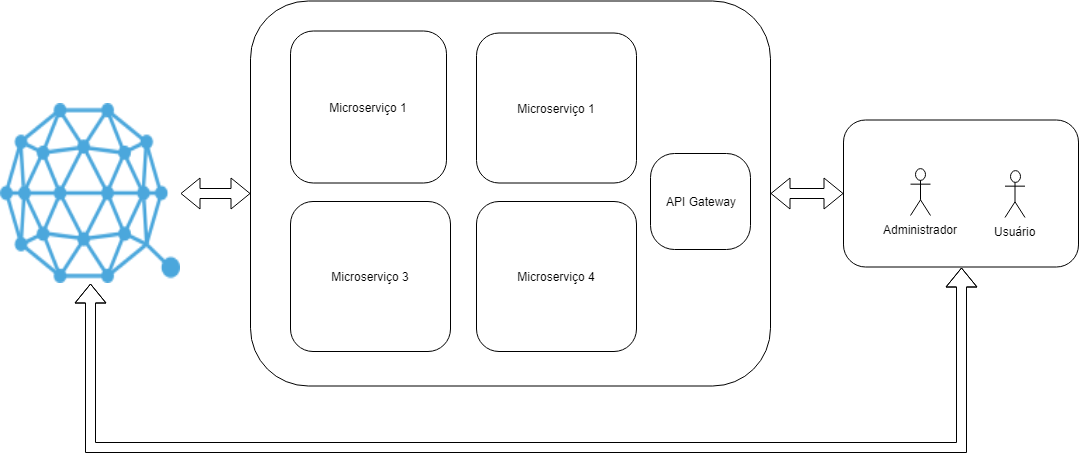
\includegraphics[width=0.7\textwidth]{Cap1/arquitetura_1_generica}
\caption{Arquitetura 1: Todos os dados pertinentes ao contrato estão no blockchain.}
\label{arquitetura_1_generica}
\end{figure}

\begin{figure}[ht]
\centering
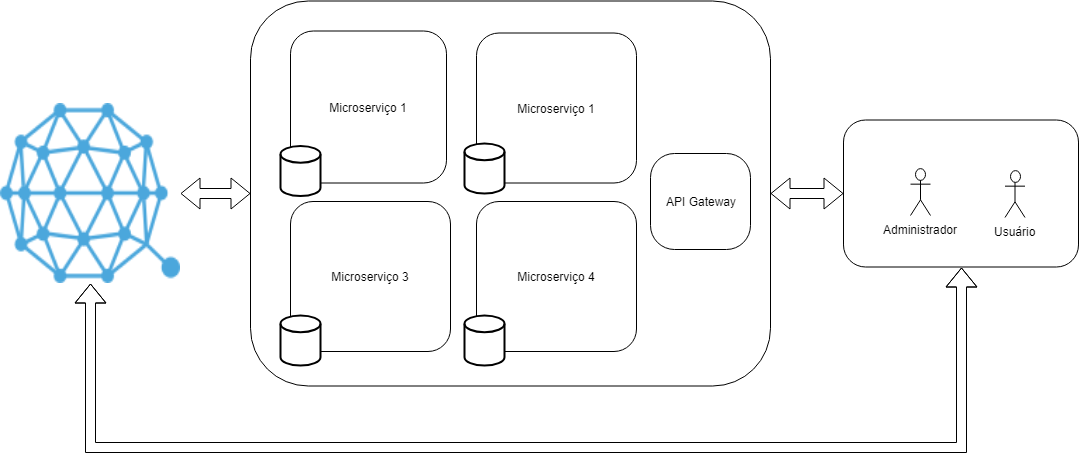
\includegraphics[width=0.7\textwidth]{Cap1/arquitetura_2_generica}
\caption{Parte dos dados está no blockchain e outra parte dos dados está em um banco de dados tradicional.}
\label{arquitetura_2_generica}
\end{figure}

Devido ao grande número de redes blockchain que suportam contratos inteligentes, bem como o grande número de aplicações que podem ser construídas com o uso de contratos inteligentes, a comparação das duas arquiteturas propostas será feita especificamente para uma aplicação de um seguro automotivo baseado em um contrato inteligente hospedado no blockchain Ethereum.

\section{Blockchain 1.0}

Blockchain 1.0 se refere a aplicação do blockchain para construção de moedas digitais, cryptomoedas \cite{blockchainneweconomy}. A mais famosa delas é o Bitcoin, cuja especificação técnica se encontra no paper de Satoshi Nakamoto \cite{paper_satoshi}. Nesta seção será explicado os mecanismos básicos do blockchain 1.0 especicíficos do Bitcoin.

\subsection{O Paper de Satoshi Nakamoto}

Neste paper, Satoshi Nakamoto propõem a construção de uma moeda digital, Bitcoin, baseada em uma rede peer to peer, na qual as transações são assinadas digitalmente e o problema do gasto duplo é resolvido por meio da construção de uma cadeia de blocos que armazenam as transações em ordem cronológica. A construção e aceitação de tais blocos é feito de modo que se mais da metade do poder de processamento da rede em questão for honesto, as transações serão válidas.

\subsection{Transações}

De uma forma simplificada, cada transação de certa quantia de bitcoin no blockchain 1.0 conterá \cite{bitcoin_transaction}:

\begin{itemize}
\item O hash da transação anterior, que transferiu o bitcoin para o dono atual
\item A chave pública do dono atual do bitcoin
\item A assinatura do dono atual do bitcoin sobre o hash de uma versão simplificada da transação
\item O hash da chave pública do futuro dono do bitcoin
\item A quantia de bitcoin que será transferida na transação em questão
\end{itemize}

\begin{figure}[ht]
\centering
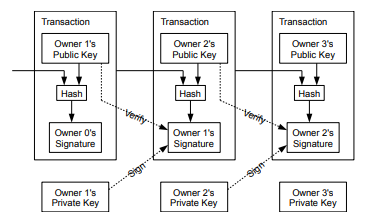
\includegraphics[width=0.5\textwidth]{Cap1/blockchain_transactions}
\caption{Transações em um blockchain.}
\label{blockchain_transactions}
\end{figure}

Apesar dessa solução garantir que uma transação ocorra apenas se o dono dela autorizar, por meio de uma assinatura ECDSA (Elliptic Curve Digital Signature Algorithm). Ela ainda não resolve o problema do gasto duplo. Para resolver esse problema, todos os nós da rede devem estar cientes de todas as transações e em caso de gastos duplo, os nós também concordar qual será considerada a transação válida.

\subsection{Servidor Timestamp}

Para evitar o problema do gasto duplo, o bitcoin utilizar um servidor timestamp, que faz com que as transações sejam agrupadas em blocos e cada bloco possuirá seu hash, que dependerá do hash do bloco anterior, das transações dentro daquela bloco e do tempo no qual aquele bloco foi criado. Dessa forma, cada nó garante uma ordem cronológica na ocorrência das transações e pode, em caso de gasto duplo, determinar qual transação será considerada a transação válida.

\begin{figure}[ht]
\centering
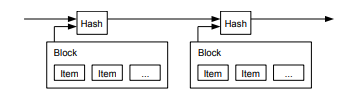
\includegraphics[width=0.5\textwidth]{Cap1/blockchain_timestamp}
\caption{Servidor Timestamp.}
\label{blockchain_timestamp}
\end{figure}

\subsection{Prova de Trabalho}

Para garantir concordância entre os nós da rede, a cadeia de blocos mais longa é considerada como sendo a verdadeira. Para evitar que algum nó crie uma transação inválida ou modifique uma transação anterior, a criação de cada bloco exige que o nó que está criando aquele bloco varie certos valores do bloco de modo que o hash do bloco inicie com determinado número de zeros. Como o hash de cada bloco depende do hash anterior, se algum nó quiser adicionar uma transação inválida ou modificar um bloco anterior, ele deverá construir os blocos mais rápidos que os outros nós da rede. 

Dessa forma, cada nó da rede que participa da criação de blocos (mineradores) fica variando certos valores do bloco até encontrar um hash válido ou até um outro nó encontre um hash válido antes dele.

\begin{figure}[ht]
\centering
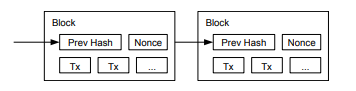
\includegraphics[width=0.5\textwidth]{Cap1/pow}
\caption{Prova de trabalho.}
\label{pow}
\end{figure}

O número de zeros que o hash de cada bloco deve ter é ajustado de modo que a criação de cada bloco leve em média 10 minutos, conforme pode-se observar na figura \ref{block_avg_time} \cite{time_avg_block}.

\begin{figure}[ht]
\centering
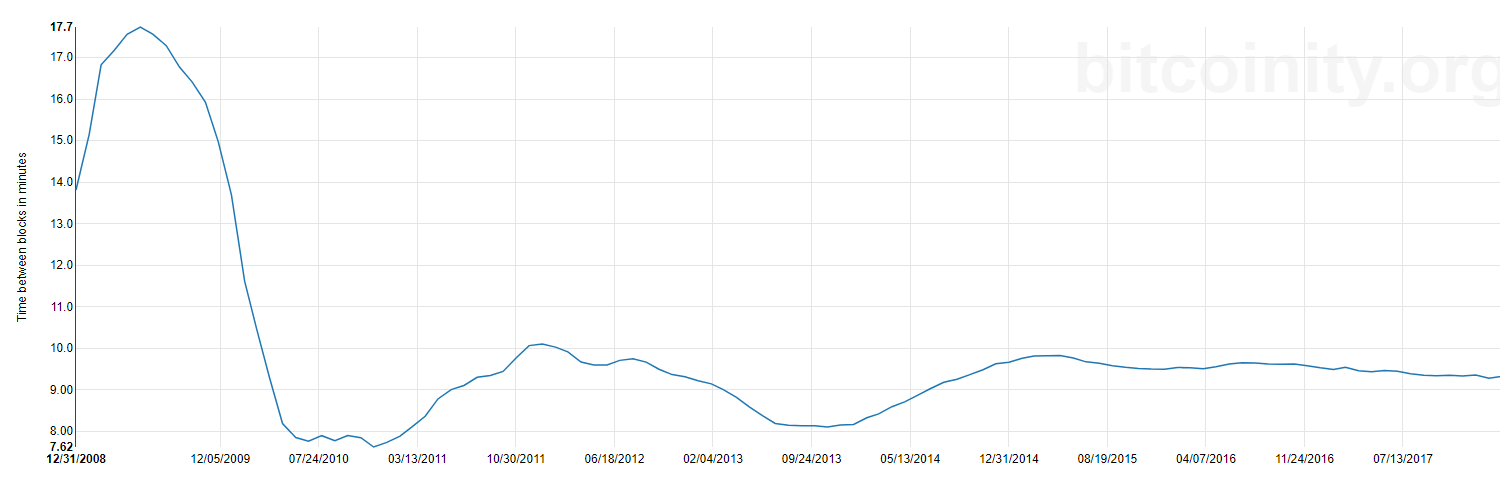
\includegraphics[width=1\textwidth]{Cap1/block_avg_time}
\caption{Tempo de geração de um novo bloco.}
\label{block_avg_time}
\end{figure}

\subsection{Rede}

Os nós de uma rede blockchain 1.0 apresentam o seguinte comportamento \cite{paper_satoshi}:

\begin{itemize}
\item Novas transações são emitidas para todos os nós
\item Cada nó coleta as transações em um bloco
\item Cada nó trabalha para encontrar o hash do seu bloco, prova de trabalho
\item Quando um nó encontra sua prova de trabalho, ele emite o bloco para todos os nós
\item Cada nó aceita um bloco apenas se todas as transações forem válidas (assinadas e sem gastos duplos)
\item Ao aceitar um bloco, os nós começam a trabalhar na prova de trabalho do próximo bloco, considerando o hash do último bloco aceito.

\end{itemize}

\subsection{Incentivo}

Para incentivar a entrada e permanência de novos nós na rede e introduzir novas moedas bitcoins ao mercado, cada novo bloco criado gerará uma certa quantia de bitcoins que poderá ser creditada em uma conta determinada pelo nó que resolveu a prova de trabalho do bloco em questão.

\subsection{Combinando e Particionando Valor}

A origem dos bitcoins em cada transação pode advir de múltiplas saídas de outras transações, bem como cada transação pode conter múltiplos destinos para o envio dos bitcoins.

\begin{figure}[ht]
\centering
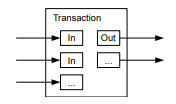
\includegraphics[width=0.3\textwidth]{Cap1/value_partition}
\caption{Combinando e particionando valor.}
\label{value_partition}
\end{figure}

\subsection{Privacidade}

Como o credor e creditado de cada transação é específicado por uma chave pública, não há como determinar a identidade das pessoas/instituições que fazem/recebem as transações. Desse modo, em uma rede blockchain 1.0, as transações são públicas, mas a identidade das pessoas/instituições é preservada.

\section{Blockchain 2.0}

Blockchain 2.0 se refere a aplicação do blockchain para construção de contratos inteligentes \cite{blockchainneweconomy}. A blockchain 2.0 mais famosa é a Ethereum, cuja proposta se encontra no paper escrito por Vitalik Buterin \cite{paper_ethereum}.

\subsection{O Paper de Vitalik Buterin}

Neste paper, Vitalik propõem a criação de uma nova versão do blockchain. Ele mostra que o blockchain pode ser visto como uma máquina de transição de estados e extende o conceito de blockchain de Nakamoto criando o Ethereum, uma rede blockchain na qual cada mudança de estado é executada por uma máquina virtual Turing-completa. Em uma rede blockchain 2.0 como Ethereum, além de armazenar dados de transações monetárias (na moeda Ether) ela também é capaz de armazenar e de processar qualquer tipo de dado, aumentando assim a gama de aplicações possíveis.

\begin{figure}[ht]
\centering
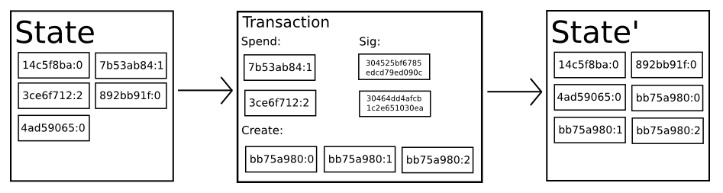
\includegraphics[width=0.8\textwidth]{Cap1/blockchain_as_state_transition_machine}
\caption{Blockchain como uma máquina de transição de estados.}
\label{blockchain_as_state_transition_machine}
\end{figure}

\subsection{Aplicações com Ethereum}

A possibilidade de se executar código no blockchain possibilita a criação de diversas aplicações, entre elas:

\subsubsection{Sistemas de Token}

Sistemas de token são como moedas de troca para um determinado ecossistema e possuem como operação básica a transferência do token de uma conta para outra:

\begin{minted}{python}
def send(to, value):
    if self.storage[msg.sender] >= value:
        self.storage[msg.sender] = self.storage[msg.sender] - value
        self.storage[to] = self.storage[to] + value
\end{minted}

\subsubsection{Domain Name Service}

Uma outra aplicação para o Ethereum é construção de uma base de dados pública para o armazenamento de domínios, o contrato dessa aplicação possuiria uma operação para registrar novos domínios:

\begin{minted}{python}
def register(name, value):
    if not self.storage[name]:
        self.storage[name] = value
\end{minted}

\subsection{Contas no Ethereum}

No Ethereum, toda transição de estado é marcada pela transição de valor ou dado de uma conta Ethereum. Toda conta Ethereum possui quatro campos:

\begin{itemize}
\item Nonce: Inteiro incrementado em cada transação da conta em questão
\item Balanço: A quantia de Ether que essa conta possui
\item Contrato: Código de contrato dessa conta, caso possua
\item Storage: Contém os dados persistentes dessa conta
\end{itemize}

Conforme pode-se observar nos campos acima, uma conta Ethereum pode ser gerenciada por uma pessoa ou por um código. No caso em que a conta é gerenciada por um código, diz-se que a conta é um contrato.

\subsection{Mensagens e Transações no Ethereum}

Transações podem enviar Ether para uma conta ou então ativar o contrato de alguma conta. Toda transação deve ser assinada por seu emissor e possui os seguintes campos:

\begin{itemize}
\item O receptor da transação
\item A assinatura identificando o emissor
\item A quantia de Ether que será fornecida
\item Startgas: Valor que representa quantos passos computacionais essa transação está permitida a fazer
\item Gasprice: Valor que representa o quanto o emissor está disposto a pagar por passo computacional
\end{itemize}

Para evitar loopings infinitos sendo executados nos contratos, cada transação deve fornecer uma quantia de Ether proporcional à quantia de passos computacionais que tal transação consumirá. Dessa forma, se algum usuário malicioso criar um contrato com um looping infinito e atrasar o processamento da rede, ele terá que pagar por isso.

As mensagens são semelhantes às transações, porém são utilizadas para que contratos interajam com outros contratos.

\subsection{Função de Transição de Estado no Ethereum}

Uma transição de estado no Ethereum segue os seguintes passos:

\begin{enumerate}
\item Checa-se se a transação é válida: possui o número correto de parâmetros, a assinatura é válida e o nonce da transação corresponde ao nonce da conta.
\item Calcula-se a taxa da transação (\(STARTGAS * GASPRICE\)) e a debita o valor da conta do remetente da transação, bem como incrementa o nonce do remetente
\item Inicializa-se \(GAS = STARTGAS\) e debita de \(GAS\) o valor correspondente ao custo do transporte de dados da transação em questão
\item Transfere-se o valor especificado na transação do remetente para o destinatário, caso a conta destinatária não exista, ela é criada.
\item Caso o remetente não tenha fundos suficientes ou a execução do código já consumiu toda quantia de gás fornecida, todas as alterações em contas afetadas devem ser revertidas e as taxas de gas devem ser creditadas na conta de quem minerou o bloco.
\item Caso a transação ocorra normalmente, a quantia de ether em forma de gas que não foi consumida é creditada na conta do remetente da transação.
\end{enumerate}

\begin{figure}[ht]
\centering
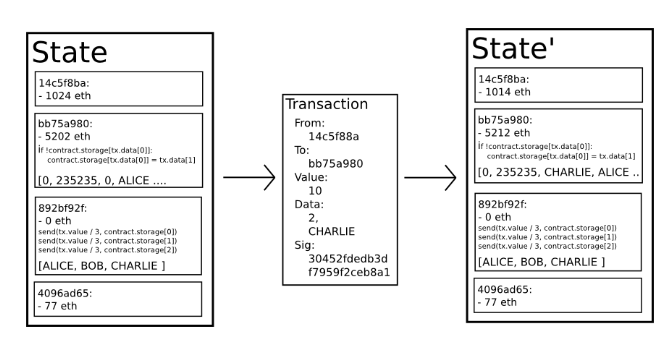
\includegraphics[width=0.8\textwidth]{Cap1/ethereum_state_transiction_function}
\caption{Diagrama de uma transição de estado no Ethereum.}
\label{ethereum_state_transiction_function}
\end{figure}

\subsection{Execução de Código no Ethereum}

Os códigos de contratos no Ethereum são criados em linguagens de alto nível, como Solidity (semelhante a JavaScript) e Serpent (semelhante a Python) e são compilados para uma linguagem de baixo nível em bytecode que será interpretada pela EVM (Ethereum Virtual Machine).

\begin{figure}[ht]
\centering
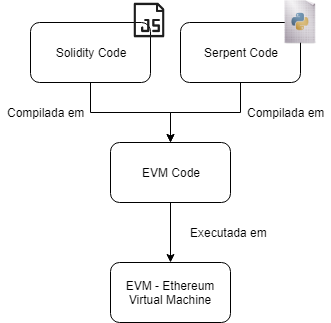
\includegraphics[width=0.5\textwidth]{Cap1/ethereum_compilation_and_execution}
\caption{Compilação e execução no ambiente Ethereum.}
\label{ethereum_compilation_and_execution}
\end{figure}

A EVM executa EVM code, uma linguagem bytecode de baixo nível baseada em pilha. O estado computacional da EVM é determinado a partir de 5 parâmetros \cite{ethereum_yellow_paper}:

\begin{itemize}
\item g: Quantia de gás disponível
\item pc: Contador do programa
\item m: Conteúdo na memória temporária
\item i: O número de palavras na memória
\item s: O conteúdo da pilha
\end{itemize}

\section{Microserviços}

De acordo com Sam Newman \cite{building_microservices}, uma arquitetura baseada em microserviços se dá por uma abordagem na qual uma aplicação é dívidida em n serviços com ciclo de vida próprio e com responsabilidades específicas. Tais serviços cooperam entre si e juntos formam a aplicação como um todo.

\subsection{Características desejáveis de um microserviço}

\begin{itemize}
\item Pequenos e focados em fazer apenas uma coisa: Os microserviços devem ser baseados em domínios de negócio da aplicação em questão, garantindo que a base de código de cada microserviço não cresça indeterminadamente e garantindo que os programadores saibam exatamente qual microserviço é responsável por determinada tarefa.
\item Autonomia: Cada microserviço pode ser colocado em produção de forma independente, os microserviços interagem entre si por meio de chamadas de API na rede.
\end{itemize}

\subsection{Vantagens de se utilizar microserviços}

\begin{itemize}
\item Heterogeneidade de tecnologia: Como cada microserviço é independente um do outro, cada microserviço pode ser constrúido com uma tecnologia específica. Por exemplo, o microserviço A pode utilizar a linguagem Python e um banco de dados relacional, como PostgreSQL. Já um segundo microserviço B, poderia utilizar a linguagem Go e um banco de dados não relacional, como MongoDB.
\item Resiliência: Se um microserviço falhar, a aplicação como um todo não será comprometida. Apenas o microserviço em questão e as funcionalidades que dependem dele estarão indisponíveis.
\item Facilidade para deploy: Ao alterar o código de um microserviço, pode-se colocar tal mudança em produção rapidamente com um risco menor de se inserir falhas, dado que você alterou apenas uma parte específica e isolada da aplicação.
\item Alinhamento Organizacional: A responsabilidade por cada microserviço pode ser atribuída a um time específico, tornando mais claro a responsabilidade de cada time e como os times devem se alinhar para interagirem com as funcionalidades criadas por outro time.
\item Otimizado para mudanças: Caso seja necessária uma mudança grande na aplicação, essa mudança será gradualmente implementada, um microserviço por vez, reduzindo os riscos de tal mudança.
\end{itemize}

\section{API's REST}

Devido à necessidade de escalabilidade, interação de componentes, generalidade de interface, independência de deploys e mudanças da World Wide Web, Roy Fielding formaliza \cite{royrest} a proposta de uma arquitetura que atenda tais necessidades. Tal arquitetura ficou conhecida como REST (REpresentational State Transfer) e é baseada em 6 pricípios:

\subsection{Modelo cliente-servidor}

Nesse modelo, cliente e servidor podem evoluir independentemente um do outro. As preocupações com a interface do usuário estarão desacopladas das preocupações com o armazenamento de dados, possibilitando interfaces de usuários em múltiplas plataformas com a mesma base de dados.

\begin{figure}[ht]
\centering
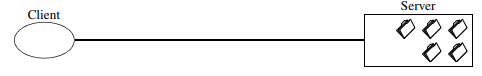
\includegraphics[width=0.5\textwidth]{Cap1/rest_client_server}
\caption{Modelo cliente-servidor}
\label{rest_client_server}
\end{figure}

\subsection{Stateless}

Cada request do cliente para o servidor deve conter toda informação necessária. Com isso aumenta-se a  visibilidade pois uma análise da interação cliente e servidor irá conter apenas um request. A confiabilidade do sistema também aumenta, pois o estado/sessão será mantido no cliente e qualquer problema no servidor não o afetará. Isso também aumenta a escalabilidade, pois o servidor não irá despender recursos para armazenar o estado/seção dos usuários.

\begin{figure}[ht]
\centering
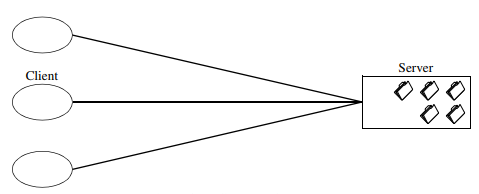
\includegraphics[width=0.5\textwidth]{Cap1/rest_stateless}
\caption{Stateless}
\label{rest_stateless}
\end{figure}

\subsection{Cache}

Para poupar os recursos de rede e/ou computação no servidor, quando o cliente ou servidor já possuir uma copia suficientemente atualizada do recurso requisitado, o recurso armazenado na cache será utilizado. Com isso aumentamos a escalabilidade do sistema e a percepção de velocidade pelo usuário final.

\begin{figure}[ht]
\centering
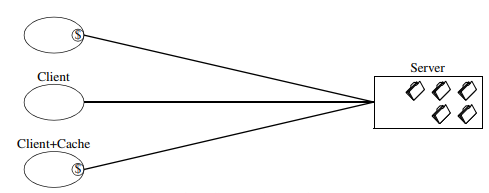
\includegraphics[width=0.4\textwidth]{Cap1/rest_cache}
\caption{Cache}
\label{rest_cache}
\end{figure}

\subsection{Interface Uniforme}

Ao definir e utilizar uma interface única para comunicação entre os componentes do sistema, a arquitetura do sistema é simplificada e compreende-lo se torna mais claro.

\begin{figure}[ht]
\centering
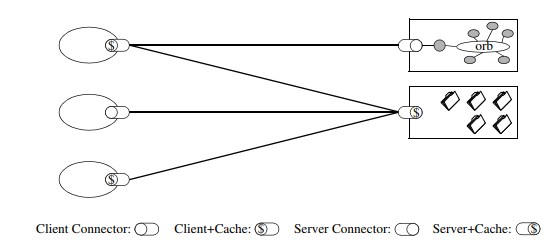
\includegraphics[width=0.5\textwidth]{Cap1/rest_uniform_interface}
\caption{Interface uniforme}
\label{rest_uniform_interface}
\end{figure}

\subsection{Sistema Baseado em Camadas}

Embora adicionem uma latência maior para o processamento de dados, um sistema baseado em camadas promove uma maior independência entre os componentes do sistema.

\begin{figure}[ht]
\centering
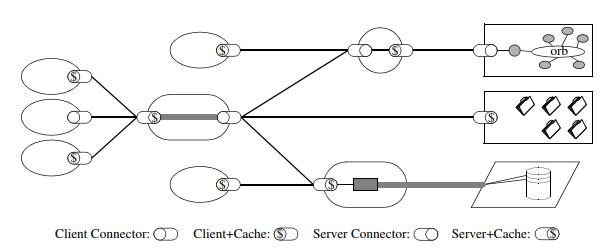
\includegraphics[width=0.5\textwidth]{Cap1/rest_layer_based_system}
\caption{Sistema baseado em camadas}
\label{rest_layer_based_system}
\end{figure}

\subsection{Código sob Demanda}

As funcionalidades e comportamentos dos clientes podem ser extendidos com o download de scripts que estão no servidor. Dessa forma, o cliente é simplificado, no sentido de exigir uma menor quantia de features pré-implementadas.

\begin{figure}[ht]
\centering
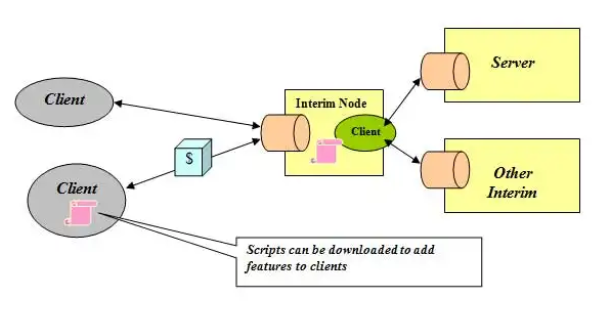
\includegraphics[width=0.5\textwidth]{Cap1/rest_code_on_demand}
\caption{Código sob demanda}
\label{rest_code_on_demand}
\end{figure}

\section{Estudo de Caso: Um seguro automotivo baseado em um contrato inteligente}

A aplicação que será construída e que proverá os dados para análise e comparação é a de um seguro automotivo, contra furto e roubo, baseado em Ethereum. O seguro se dará por meio de um contrato inteligente hospedado na rede de teste Rinkeby e por meio de microserviços que irão interagir com as partes envolvidas.

Serão construídas e comparadas duas arquiteturas. Na primeira delas (figura \ref{arquitetura_1}), todos os dados pertinentes estarão no blockchain. Já na segunda arquitetura (figura \ref{arquitetura_2}), parte dos dados estará no blockchain e outra parte dos dados estará em um banco de dados tradicional administrado pelo seguro.

\begin{figure}[ht]
\centering
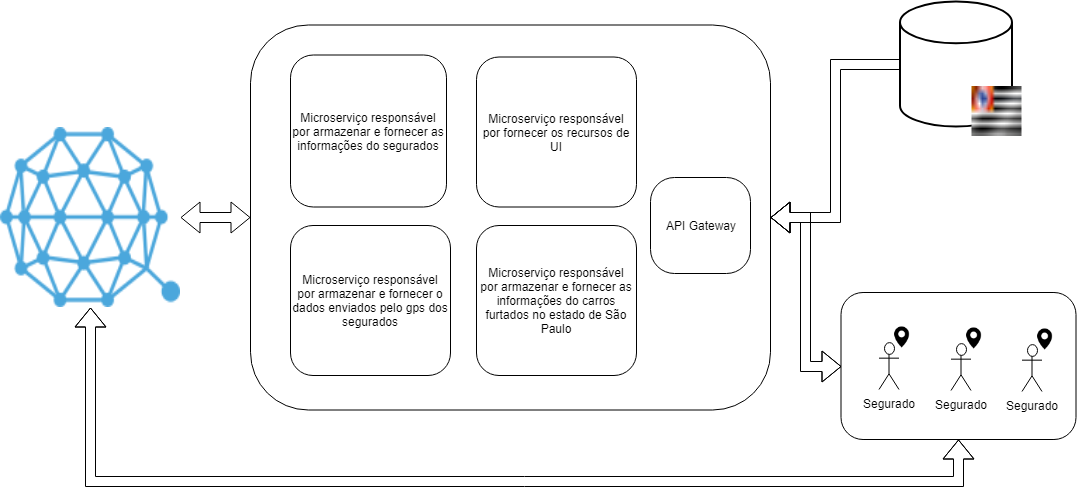
\includegraphics[width=0.8\textwidth]{Cap1/arquitetura_1}
\caption{Arquitetura 1: Todos os dados estão armazenados no blockchain.}
\label{arquitetura_1}
\end{figure}

\begin{figure}[ht]
\centering
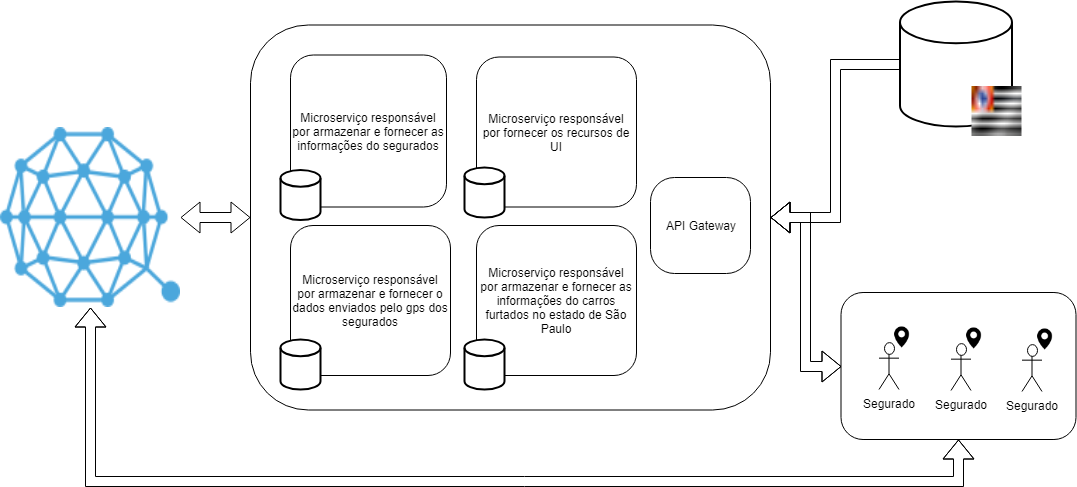
\includegraphics[width=0.8\textwidth]{Cap1/arquitetura_2}
\caption{Arquitetura 2: Parte dos dados está no blockchain e outra parte está em um banco de dados tradicional administrado pelo seguro.}
\label{arquitetura_2}
\end{figure}

\subsection{Partes envolvidas no seguro}

\begin{itemize}
\item Segurado: Responsável por
	\begin{itemize}
	\item Se cadastrar no seguro
    \item Enviar mensalmente a quantia acordada em Ethereum
    \item Instalar um dispositivo que envie em tempo real a localização de seu carro
    \item Iniciar o processo de reembolso em caso de roubo ou furto
	\end{itemize}
\item Seguro: Responsável por
	\begin{itemize}
	\item Disponibilizar um Website no qual as pessoas possam aderir ao seguro e acompanhar seus dados pessoais e os dados do seguro
    \item Criar e manter os contratos inteligentes na rede Ethereum
    \item Disponibilizar uma API para receber os dados de localização dos carros dos segurados
    \item Obter e cadastrar no sistema do seguro os carros furtados no Estado de São Paulo
	\end{itemize}
\item Governo do estado de São Paulo: Responsável por
	\begin{itemize}
	\item Disponibilizar um banco de dados com os dados de furtos e roubos de carros no Estado de São Paulo
	\end{itemize}
\end{itemize}

\subsection{O Contrato Inteligente}

O seguro será responsável por elaborar o código de dois contratos:

\begin{enumerate}
\item AutoInsuranceFactory: Responsável por
	\begin{itemize}
	\item Criar os contratos do seguro (AutoInsurance)
    \item Armazenar todos os contratos já criados e quem os criou
	\end{itemize}
\item AutoInsurance: Responsável por
	\begin{itemize}
	\item Armazenar o dinheiro enviado pelos segurados, em Ethereum
    \item Reembolsar o segurado em caso de roubo ou furto. O reembolso só será efetuado caso um boletim de ocorrência seja efetuado e disponibilizado no banco de dados do Governo do Estado de São Paulo. Um outro critério para a liberação do reembolso é o de que o local e hora do roubo ou furto registrado no B.O. coincida com os dados enviados pelo dispositivo instalado no carro do segurado.
	\end{itemize}
\end{enumerate}

\section{BIP32 \& BIP39}

Para garantir a privacidade dos usuários, os dados enviados pelo dispositivo GPS serão criptografados, de modo que cada amostra do sinal GPS será criptografado e descriptografado por uma mesma chave privada. Desse modo, o usuário terá o controle de privacidade de cada amostra, podendo fornecer a chave privada de amostras específicas do dispositivo GPS.

Para gerar múltiplas chaves privadas para cada amostra de sinal GPS é utilizado o BIP32.

\subsection{BIP32}

BIP32 \cite{github_bip32}, ``Bitcoin Improvement Proposal number 32'', é, de acordo com \cite{deployability_bitcoin_bip32}, uma técnica utilizada para geração de uma árvore de endereços bitcoin (chave pública e chave privada) a partir de uma chave semente, conhecida como ``Master Seed''. A partir da ``Master Seed'', um nó mestre é gerado e a partir do nó mestre, outros nós podem ser gerados. Na figura \ref{hd_tree}, pode-se ver o exemplo de uma árvore gerada pelo BIP32.

\begin{figure}[ht]
\centering
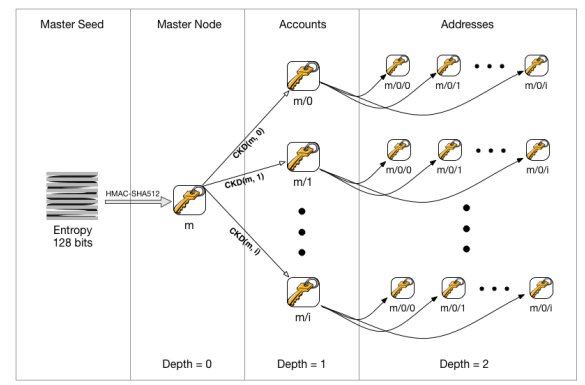
\includegraphics[width=0.9\textwidth]{Cap1/hd_tree}
\caption{BIP32: Árvore de endereços bitcoin.}
\label{hd_tree}
\end{figure}

\subsubsection{Chave extendida}

Para evitar que as chaves filhas dependam somente das chaves mãe, é utilizado o conceito de chaves extendidas. Uma chave extendida nada mais é do que uma chave pública ou privada acompanhada de 256 bits de entropia, esses 256 bits de entropia é conhecido como ``chain code''. Neste caso, uma chave privada extendida é obtida a partir do par ordenado (k, c), sendo k a chave privada e c o ``chain code''.

\subsubsection{Geração do nó mestre}

O nó mestre é obtido indiretamente a partir de S, também conhecido como ``master seed'':

\begin{enumerate}
\item Gerar uma sequência de bytes S (entre 128 e 512 bits);
\item Calcular I = HMAC-SHA512(Key = "Bitcoin seed", Data = S);
\item Separar I em duas arrays de 32 bytes, I = I\textsubscript{l} || I\textsubscript{r};
\item I\textsubscript{l} representará a chave privada mestre e I\textsubscript{r} representará o ``chain code''  mestre.
\end{enumerate}

\subsubsection{Geração de uma chave privada filha}

As chaves privadas filhas são geradas a partir da chave privada mãe extendida segundo a função: 
\[CKDpriv((k_{par}, c_{par}), i) \rightarrow (k_{i}, c_{i})\]

CKDpriv é obtido a paritr do seguintes passos:

\begin{enumerate}
\item Checar se i (índice do filho) é maior que 2\textsuperscript{31}:
  \begin{itemize}
  \item Se sim (``hardened child''), I = HMAC-SHA512(Key = c\textsubscript{par}, Data = 0x00 || ser\textsubscript{256}(k\textsubscript{par}) || ser\textsubscript{32}(i))
  \item Caso contrário (``normal child''), I = HMAC-SHA512(Key = c\textsubscript{par}, Data = ser\textsubscript{256}(k\textsubscript{par}) || ser\textsubscript{32}(i)) 
  \end{itemize}
\item Separar I em duas arrays de 32 bytes, I = I\textsubscript{l} || I\textsubscript{r};
\item k\textsubscript{i} = parse\textsubscript{256}(I\textsubscript{l}) + k\textsubscript{par} (mod n), onde n é ordem da curva secp256k1 \cite{secp256k1};
\end{enumerate}

\subsection{BIP39}

BIP39 \cite{github_bip39}, ``Bitcoin Improvement Proposal number 39'', é, de acordo com \cite{fornaro_thesis}, uma técnica utilizada para obter a ``Master seed'' a partir de uma frase mnemônica. Uma frase mnemônica nada mais é do que uma lista ordenada de palavras tiradas de determinado dicionário. Os passos para se obter o mnemônico  partir de uma entrada aleatória podem ser vistos na figura \ref{bip39_to_mnemonic} e os passos para se obter o ``Seed'' a partir do mnêmonico podem ser observados na figura \ref{bip39_to_seed}.

\begin{figure}[ht]
\centering
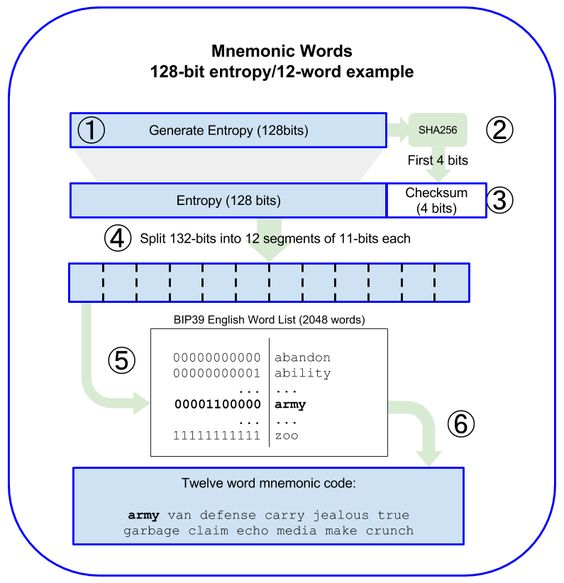
\includegraphics[width=0.8\textwidth]{Cap1/bip39_to_mnemonic}
\caption{Geração do mnemônico.}
\label{bip39_to_mnemonic}
\end{figure}

\begin{figure}[ht]
\centering
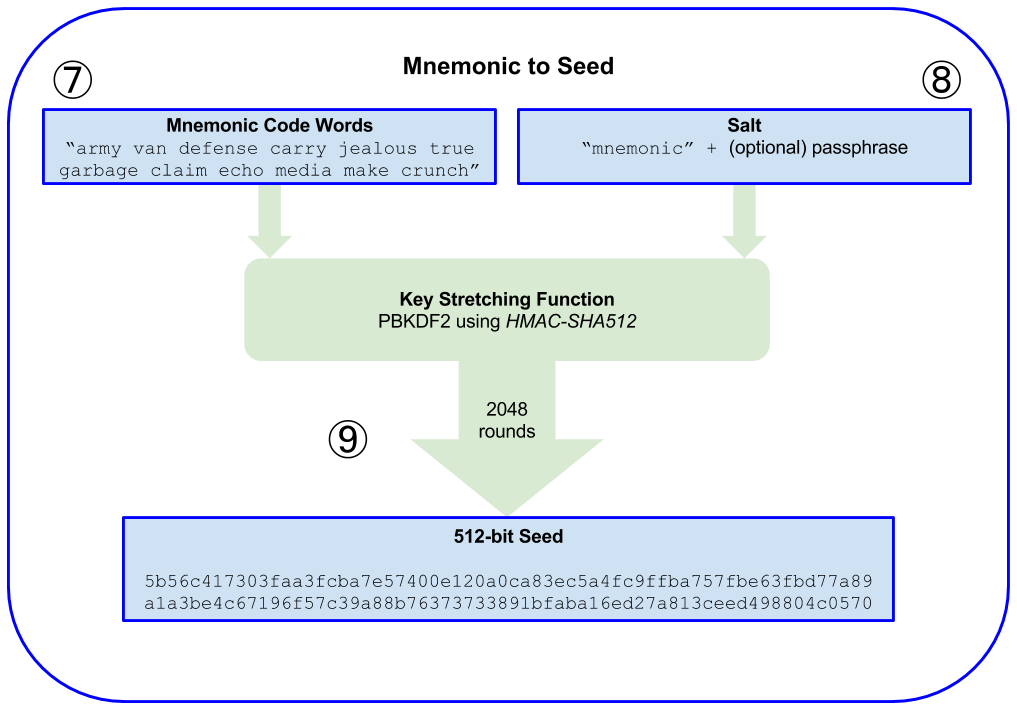
\includegraphics[width=0.8\textwidth]{Cap1/bip39_to_seed}
\caption{Obtenção do ``seed'' a partir do mnemônico.}
\label{bip39_to_seed}
\end{figure}

%vê o problema de controle tolerante a falhas através de uma perspectiva integrada, foi proposta por
%{marcel4}. Os autores apresentam um ambiente híbrido consistindo de três unidades básicas que garantem a compleição de tarefas na presença de qualquer número de juntas falhas (Figura \ref{cupim}). A primeira unidade é um esquema de detecção
%e isolação de falhas que continuamente monitora o manipulador para detectar e identificar possíveis falhas nas juntas. A segunda unidade é responsável pela reconfiguração do controle. A terceira unidade é composta de algorítmos de
%controle apropriados para cada tipo de configuração do robô, baseado na informação da unidade de reconfiguração \cite{COFFEE2000}.

%Segundo, o critério de otimização utilizado será o acoplamento entre as juntas do
%manipulador e neste caso, temos um sistema redundante quando ocorre falha de uma das juntas do manipulador de três juntas, e seu posicionamento é controlado pelas duas restantes. Nossa solução para o problema é baseada na formulação
%inversa ({nakamura}). A

%\begin{figure}[ht!]
%\centering
%\includegraphics[width=1\textwidth]{Cap1/cupimconcreto}
%\caption{Exemplo real de cupim frente ao seu dilema.}
%\label{FDII}
%\end{figure}

\chapter{Desenvolvimento}
Essa seção tem como objetivo detalhar o desenvolvimento da aplicação do seguro automotivo com as duas arquiteturas propostas e apresentar a metodologia utilizada para comparar a performance e o custo dessas duas arquiteturas.

\section{Construção do seguro automotivo utilizando a arquitetura baseada 100\% na rede Ethereum}

\subsection{Arquitetura e tecnologias utilizadas}

\begin{figure}[h]
\centering
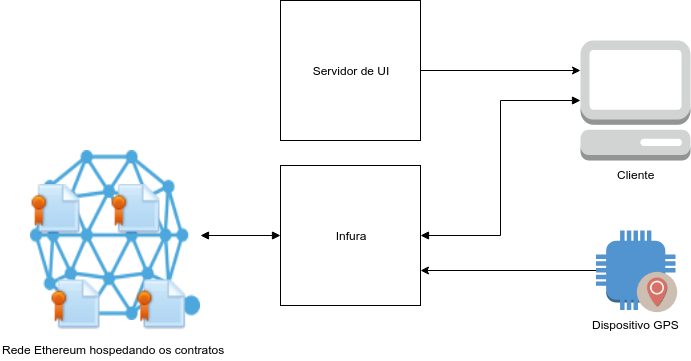
\includegraphics[width=0.7\textwidth]{Cap2/full_ethereum_architecture.png}
\caption{Arquitetura baseada 100\% na rede ethereum.}
\label{full_ethereum_architecture}
\end{figure}

Como pode-se observar na figura \ref{full_ethereum_architecture}, essa arquitetura é composta por 5 componentes:

\begin{itemize}
	\item \textbf{Cliente:} O cliente representa a aplicação web desenvolvida com a framework React (\href{http://www.reactjs.org}{http://www.reactjs.org}) e é responsável por criar um interface gráfica na qual as pessoas possam observar e interagir com os contratos de uma forma amigável.
    \item \textbf{Servidor de UI:} É um servidor de recursos estáticos desenvolvido em Nodejs (\href{http://www.nodejs.org}{http://www.nodejs.org}) com a framework Express (\href{http://www.express.com}{http://www.express.com}). Tal servidor provê o arquivo javascript que contém o código do cliente desenvolvido em React, bem como as imagens da aplicação web.
    \item \textbf{Infura:} Infura (\href{https://infura.io/}{https://infura.io/}) é um serviço web que prove acesso a rede Ethereum por meio de uma API REST. Esse serviço abstrai a complexidade de criar e manter um nó próprio conectado a rede Ethereum.
    \item \textbf{Rede Ethereum:} Representa a rede Ethereum composta por nós espalhados pelo mundo todo.
    \item \textbf{Contratos:} Representa os contratos de seguro automotivo criados e mantidos pelos usuários da aplicação.
    \item \textbf{Dispositivo GPS:} O dispositivo GPS é responsável por enviar constantemente a localização do carro dos participantes do contrato de seguro automotivo para a rede Ethereum. Para manter a privacidade dos usuários, o envio da latitude e longitude é criptografado.
\end{itemize}

Nas seções abaixo, será dado enfoque nos principais componentes do sistema: os contratos, o cliente e o dispositivo GPS.

\subsection{Contratos}

Foram desenvolvidos dois contratos inteligentes, o primeiro deles, SmartCarInsuranceContractFactory, é um contrato responsável por criar e rastrear todos contratos de seguro automotivo. Já o segundo contrato desenvolvido, SmartCarInsuranceContract, representa o próprio contrato de seguro automotivo. O código completo dos contratos está disponível no GitHub (\href{https://github.com/marcoprado17/scife-contracts}{https://github.com/marcoprado17/scife-contracts}).

\begin{figure}[h!]
\centering
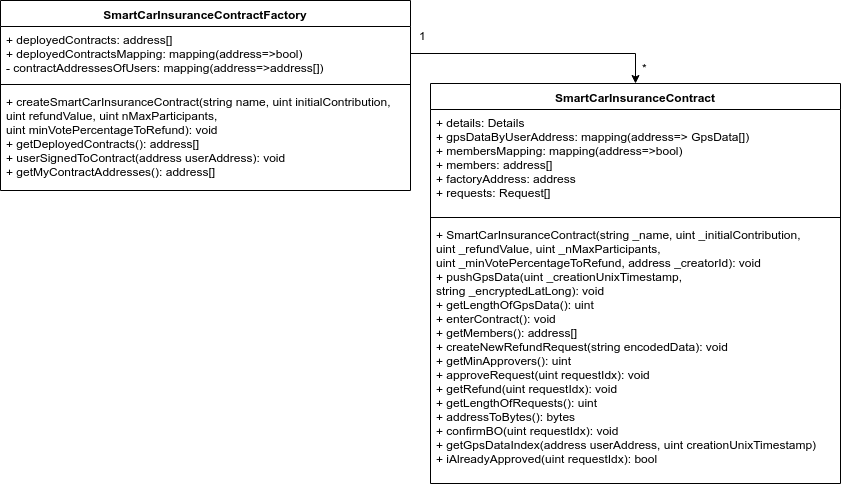
\includegraphics[width=1\textwidth]{Cap2/SmartCarInsuranceContractFactory_and_SmartCarInsuranceContract.png}
\caption{SmartCarInsuranceContractFactory e SmartCarInsuranceContract.}
\label{factory_and_contracts}
\end{figure}

Utilizar um contrato que cria outros contratos é interessante por dois motivos:

\begin{enumerate}
\item Facilita com que os usuários façam o deploy de um novo contrato automotivo no próprio browser. Para tanto, o código do cliente interage com SmartCarInsuranceContractFactory por meio do serviço do Infura para criar um novo contrato;
\item Como todo novo SmartCarInsuranceContract é criado por SmartCarInsuranceContractFactory, o próprio contrato SmartCarInsuranceContractFactory se torna o local ideal para armazenar todos os SmartCarInsuranceContract criados.
\end{enumerate}

Conforme se observa na figura \ref{factory_and_contracts}, um contrato se asemelha muito a uma classe em uma linguagem orientada a objetos: o contrato define um modelo de uma entidade que possui diferentes atributos e métodos. Tal modelo da origem a múltiplas instâncias dessa entidade, sendo que cada instância de contrato criado possui um endereço associado na rede Ethereum.

\subsubsection{SmartCarInsuranceContractFactory}

Segue abaixo o código comentado do contrato SmartCarInsuranceContractFactory:

\begin{code}
\begin{minted}[
frame=lines,
fontsize=\footnotesize,
linenos
]{javascript}
// Utilizando a versão 0.4.17 da linguagem Solidity
pragma solidity ^0.4.17;

contract SmartCarInsuranceContractFactory {
    // Array contendo os endereços ethereum de todos os contratos 
    // SmartCarInsuranceContract que SmartCarInsuranceContractFactory 
    // gerou
    address[] public deployedContracts;
    // Hash table para checagem rápida se certo endereço 
    // ethereum representa um contrato SmartCarInsuranceContract 
    // deployado por SmartCarInsuranceContractFactory
    mapping(address => bool) public deployedContractsMapping;
    // Mapeia os contratos SmartCarInsuranceContract que cada 
    // usuário participa
    mapping(address => address[]) contractAddressesOfUsers;

    // Método que cria uma nova instância de SmartCarInsuranceContract
    function createSmartCarInsuranceContract(
        string name,
        uint initialContribution,
        uint refundValue,
        uint nMaxParticipants,
        uint minVotePercentageToRefund
    ) public {
        // Criando uma nova instância de um contrato 
        // SmartCarInsuranceContract
        address newContractAddress = new SmartCarInsuranceContract(
            name,
            initialContribution,
            refundValue,
            nMaxParticipants,
            minVotePercentageToRefund, 
            msg.sender
        );
        // Armazenando o contrato deployado em deployedContracts
        deployedContracts.push(newContractAddress);
        // Adicionando à hash table deployedContractsMapping o 
        // endereço do novo contrato deployado
        deployedContractsMapping[newContractAddress] = true;
    }

    // Obtenção de deployedContracts
    function getDeployedContracts() public view returns (address[]) {
        return deployedContracts;
    }

    // Adiciona à contractAddressesOfUsers que userAddress agora faz 
    // parte do contrato SmartCarInsuranceContract que chamou essa 
    // função (msg.sender)
    function userSignedToContract(address userAddress) public{
        // Garantindo que quem chamou userSignedToContract seja de 
        // fato um contrato SmartCarInsuranceContract deployado 
        // por SmartCarInsuranceContractFactory
        require(deployedContractsMapping[msg.sender]);
        contractAddressesOfUsers[userAddress].push(msg.sender);
    }

    // Obtendo a array contendo os endereços dos contratos 
    // SmartCarInsuranceContract que o usuário que chamou essa 
    // função participa
    function getMyContractAddresses() public view returns (address[]){
        return contractAddressesOfUsers[msg.sender];
    }
}
\end{minted}
\caption{SmartCarInsuranceContractFactory}
\label{lst:SmartCarInsuranceContractFactory}
\end{code}

\subsubsection{SmartCarInsuranceContract}

Segue abaixo o código comentado de SmartCarInsuranceContract:

\begin{code}
\begin{minted}[
frame=lines,
fontsize=\footnotesize,
linenos
]{javascript}
contract SmartCarInsuranceContract {
    // Definindo a struct Details, tal struct armazena 
    // os principais dados do contrato
    struct Details {
        // Nome do contrato
        string name;
        // Contribuição inicial para participar do contrato
        uint initialContribution;
        // Valor do reembolso em caso de furto e roubo
        uint refundValue;
        // Número máximo de participantes
        uint nMaxParticipants;
        // Percentagem mínima de votos para liberar
        // o reembolso de caso de roubo ou furto
        uint minVotePercentageToRefund;
        // Endereço ethereum do criador desse contrato
        address creatorId;
        // Número de participantes do contrato
        uint nParticipants;
    }

    // Definindo a struct GpsData, tal struct armazena
    // uma amostra dos dados de gps de um usuário do contrato
    struct GpsData {
        // Unix timestamp do bloco ethereum que recebeu 
        // tal GpsData
        uint blockUnixTimestamp;
        // Tempo em que tal amostra foi colhida, esse valor
        // é enviado pelo usuário
        uint creationUnixTimestamp;
        // String encriptada contendo a latitude e longitude 
        // dessa amostra de sinal gps
        string encryptedLatLong;
    }

    // Definindo a struct Request, tal struct representa
    // uma requisição de reembolso criado por um usuário
    // do contrato
    struct Request {
        // String base64 encoded contendo um json com as informações
        // necessárias para a requisição:
        // {
        //     unixTimesptampOfTheft: 1232143213,
        //     latTheft: 1.2231
        //     longTheft: 2.2314
        //     keysOfGpsData = [
        //         [122348763244, "secret"], # [unixTimestamp, key]
        //         [122348763244, "secret"],
        //         ...
        //     ]
        // }
        string encodedData;
        // Endereço ethereum de quem criou a requisição de reembolso
        address creatorAddress;
        // Hash table que mapeia o endereço ethereum de quem aprovou
        // tal requisição de reembolso
        mapping(address => bool) approvers;
        // Número de usuários que aprovaram tal requisição de 
        // reembolso
        uint nApprovers;
        // Bool que indica se tal requisição de reembolso foi
        // aprovada pela polícia
        bool boConfirmed;
        // Unix timestamp do bloco ethereum que recebeu essa
        // nova requisição de reembolso
        uint unixTimestampOfBlock;
        // Bool que indica se o reembolso já foi efetuado ou não
        bool refundMade;
    }

    // Detalhes desse contrato de seguro automotivo
    Details public details;
    // Hash table que armazena os dados de gps de cada
    // membro do contrato
    mapping(address => GpsData[]) public gpsDataByUserAddress;
    // Hash table que armazena o endereço ethereum dos membros
    // do contrato
    mapping(address => bool) public membersMapping;
    // Array com o endereço ethereum de todos os membros do contrato
    address[] public members;
    // Endereço ethereum do contrato SmartCarInsuranceContractFactory
    // que deu origem a este contrato
    address public factoryAddress;
    // Array contento todas as requisições de reembolso feitas
    // nesse contrato
    Request[] public requests;
    
    // Contrutor de SmartCarInsuranceContract. Serve para criar
    // uma nova instância deste contrato
    function SmartCarInsuranceContract(
        string _name,
        uint _initialContribution,
        uint _refundValue,
        uint _nMaxParticipants,
        uint _minVotePercentageToRefund,
        address _creatorId
    ) public {
        // Garantindo alguns requisitos básicos para criação do contrato
        require(_initialContribution > 0);
        require(_refundValue > 0);
        require(_nMaxParticipants > 0);
        require(_minVotePercentageToRefund >= 0 && 
        _minVotePercentageToRefund <= 100);
        // Criando os detalhes desse contrato
        details = Details({
            name: _name,
            initialContribution: _initialContribution,
            refundValue: _refundValue,
            nMaxParticipants: _nMaxParticipants,
            minVotePercentageToRefund: _minVotePercentageToRefund,
            creatorId: _creatorId,
            nParticipants: 0
        });
        // Atualizando o endereço de quem criou a instância desse contrato
        factoryAddress = msg.sender;
    }

    // Método que adiciona um novo GpsData de um membro do contrato
    function pushGpsData(
        uint _creationUnixTimestamp, 
        string _encryptedLatLong) public {
        // Garantindo que quem chamou esse método seja um membro do contrato
        require(membersMapping[msg.sender]);
        uint l = gpsDataByUserAddress[msg.sender].length;
        if(l > 0){
            // Garantindo que unix timestamp fornecido pelo gps
            // seja maior do que o timestamp da última amostra
            // de sinal gps
            require(_creationUnixTimestamp > 
                gpsDataByUserAddress[msg.sender][l-1].creationUnixTimestamp);
        }
        // Criando uma nova instância de GpsData
        GpsData memory newGpsData = GpsData({
            blockUnixTimestamp: block.timestamp,
            creationUnixTimestamp: _creationUnixTimestamp,
            encryptedLatLong: _encryptedLatLong
        });

        // Adicionando a nova instância de GpsData criada para
        // a hash table gpsDataByUserAddress
        gpsDataByUserAddress[msg.sender].push(newGpsData);
    }

    // Método para a obtenção do comprimento da array que armazena
    // os dados de gps de um usuário específico
    function getLengthOfGpsData(address _address) 
    public view returns(uint) {
        return gpsDataByUserAddress[_address].length;
    }

    // Método que um possível membro do contrato chama para participar
    // do contrato de seuro automotivo em questão
    function enterContract() public payable{
        // Garantindo que o possível membro envie, ao chamar essa
        // função, um valor igual a contribuição inicial estabelecida
        // no momento em que esse contrato foi gerado
        require(msg.value == details.initialContribution);
        // Garantindo que quem chamou essa função não seja
        // membro do contrato ainda
        require(!membersMapping[msg.sender]);
        // Garantindo que o contrato em questão ainda não excederá
        // o número máximo de participantes
        require(members.length < details.nMaxParticipants);
        // Incrmentando o número de participantes
        details.nParticipants++;
        // Adicionando o novo membro à membersMapping e members
        membersMapping[msg.sender] = true;
        members.push(msg.sender);
        // Informando a SmartCarInsuranceContractFactory que msg.sender
        // agora é um membro deste contrato
        SmartCarInsuranceContractFactory smartCarInsuranceContractFactory = 
            SmartCarInsuranceContractFactory(factoryAddress);
        smartCarInsuranceContractFactory.userSignedToContract(msg.sender);
    }

    // Obtendo a array com os endereços ethereum dos membros deste contrato
    function getMembers() public view returns (address[]) {
        return members;
    }

    // Método chamado para a criação de uma nova requisição de reembolso
    /*
        encodedData representa a base64 encode do objeto abaixo:
        {
            unixTimesptampOfTheft: 1232143213,
            latTheft: 1.2231
            longTheft: 2.2314
            keysOfGpsData = [
                [122348763244, "secret"], # [unixTimestamp, key]
                [122348763244, "secret"],
                ...
            ]
        }
     */
    function createNewRefundRequest(string encodedData) public {
        // Garantindo que quem chamou esse método (msg.sender)
        // seja um membro do contrato
        require(membersMapping[msg.sender]);
        // Criando uma nova instância da struct Request com
        // os devidos dados
        Request memory newRequest;
        newRequest.encodedData = encodedData;
        newRequest.creatorAddress = msg.sender;
        newRequest.boConfirmed = false;
        newRequest.nApprovers = 0;
        newRequest.unixTimestampOfBlock = block.timestamp;
        newRequest.refundMade = false;
        // Adicionando a instância de request criada à
        // array requests
        requests.push(newRequest);
    }

    // Obtendo o número mínimo de membros que devem aprovar
    // uma requisição de reembolso para ela ser liberada
    function getMinApprovers() public view returns (uint) {
        // Retornando 0 caso details.minVotePercentageToRefund == 0
        if(details.minVotePercentageToRefund == 0) {
            return 0;
        }
        // Retornando ceil de
        // details.minVotePercentageToRefund*details.nParticipants/100
        // caso contrário
        uint multi = details.minVotePercentageToRefund * details.nParticipants;
        bool hasRemainder = true;
        if(multi % 100 == 0){
            hasRemainder = false;
        }
        uint minApprovers = multi / 100;
        if(hasRemainder){
            minApprovers++;
        }
        return minApprovers;
    }

    // Método que um usuário chama para aprovar determinada
    // requisição de reembolso
    function approveRequest(uint requestIdx) public{
        // Garantindo que msg.sender seja um membro do contrato
        require(membersMapping[msg.sender]);
        // Garantindo que msg.sender não tenha aprovado tal
        // requisão antes
        require(!requests[requestIdx].approvers[msg.sender]);
        // Adicionando aos aprovadores da requisição o endereço
        // de msg.sender
        requests[requestIdx].approvers[msg.sender] = true;
        // Aumentando o número de pessoas que aprovaram
        // tal requisição
        requests[requestIdx].nApprovers++;
        // Efetuando o reembolso caso os três requisitos abaxo
        // sejam atendidos
        // a) O número de membros aprovadores do reembolso seja 
        // maior ou igual ao mínimo requerido;
        // b) O contrato possua uma quantia de ethereum maior ou igual
        // ao valor do reembolso;
        // c) O boletim de ocorrência de furto ou roubo já tenha
        // sido confirmado pela polícia.
        uint minApprovers = getMinApprovers();
        if(
            requests[requestIdx].nApprovers >= minApprovers
            && address(this).balance >= details.refundValue
            && requests[requestIdx].boConfirmed
        ){
            requests[requestIdx].creatorAddress.send(details.refundValue);
            requests[requestIdx].refundMade = true;
        }
    }

    // Liberando o reembolso caso todos os requisitos
    // para liberação do reembolso estejam etendidos
    function getRefund(uint requestIdx) public {
        require(requests[requestIdx].creatorAddress == msg.sender);
        require(requests[requestIdx].boConfirmed);
        uint minApprovers = getMinApprovers();
        require(requests[requestIdx].nApprovers >= minApprovers);
        require(address(this).balance >= details.refundValue);
        requests[requestIdx].creatorAddress.transfer(details.refundValue);
        requests[requestIdx].refundMade = true;
    }

    // Obtendo o comprimento da array requests
    function getLengthOfRequests() public view returns(uint) {
        return requests.length;
    }

    // Função que converte um address para bytes
    function addressToBytes(address _addr) public pure returns(bytes) {
        bytes32 value = bytes32(uint256(_addr));
        bytes memory alphabet = "0123456789abcdef";

        bytes memory str = new bytes(51);
        str[0] = "0";
        str[1] = "x";
        for (uint i = 0; i < 20; i++) {
            str[2+i*2] = alphabet[uint(value[i + 12] >> 4)];
            str[3+i*2] = alphabet[uint(value[i + 12] & 0x0f)];
        }
        return str;
    }

    // Função que confirma se o BO de furto ou roubo
    // de uma determinada requisição de reembolso foi feito
    // com sucesso
    function confirmBO(uint requestIdx) public {
        // Garantindo que o BO ainda não tenha sido confirmado
        require(!requests[requestIdx].boConfirmed);
        // Garantindo que msg.sender == 
        // "0x5e924ac15745b75e0d23afd68d1bb1adb8f43689"
        bytes memory validBoSenderAddress = 
        "0x5e924ac15745b75e0d23afd68d1bb1adb8f43689";
        bytes memory senderAddress = addressToBytes(msg.sender);
        bool validSender = true;
        for(uint i = 0; i < validBoSenderAddress.length; i++){
            if(validBoSenderAddress[i] != senderAddress[i]){
                validSender = false;
            }
        }
        require(validSender);
        // Confirmando o BO
        requests[requestIdx].boConfirmed = true;
    }

    // Obtendo o indice do GpsData na array 
    // gpsDataByUserAddress[userAddress] que foi criado
    // o mais proximo possível de creationUnixTimestamp
    function getGpsDataIndex(
        address userAddress, 
        uint creationUnixTimestamp) public view returns(uint){
        if(gpsDataByUserAddress[userAddress].length == 0){
            return 0;
        }
        if(creationUnixTimestamp <= 
        gpsDataByUserAddress[userAddress][0].creationUnixTimestamp){
            return 0;
        }
        if(
            creationUnixTimestamp >= 
            gpsDataByUserAddress[userAddress]
            [gpsDataByUserAddress[userAddress].length-1]
            .creationUnixTimestamp){
            return gpsDataByUserAddress[userAddress].length-1;
        }
        // Efetuando uma busca binária para obtenção do indice
        // de GpsData com creationUnixTimestamp mais próximo
        // do desejado
        uint low = 0;
        uint high = gpsDataByUserAddress[userAddress].length-1;
        while (low <= high) {
            uint mid = (low + high) / 2;
            if(gpsDataByUserAddress[userAddress]
            [mid].creationUnixTimestamp > 
            creationUnixTimestamp){
                high = mid - 1;
            }
            else if (gpsDataByUserAddress[userAddress][mid]
            .creationUnixTimestamp < creationUnixTimestamp){
                low = mid + 1;
            }
            else {
                return mid;
            }
        }
        return low;
    }

    // Método que retorna um bool indicando se msg.sender
    // já aprovou ou não o a requisição de índice requestIdx
    function iAlreadyApproved(uint requestIdx) public view returns (bool) {
        require(membersMapping[msg.sender]);
        return requests[requestIdx].approvers[msg.sender];
    }
}
\end{minted}
\caption{SmartCarInsuranceContract}
\label{lst:SmartCarInsuranceContract}
\end{code}

\subsection{Cliente}

O código do cliente foi desenvolvido com a framework React e encontra-se disponível no GitHub (\href{https://github.com/marcoprado17/scife-ui-service}{https://github.com/marcoprado17/scife-ui-service}). Tal aplicação web contém contém 5 páginas.

\subsubsection{Páginas da aplicação}

\begin{itemize}
\item \textbf{Home Page:} Página principal da aplicação, contém uma explicação básica de como a aplicação e contrato funciona. Um screenshot dessa página pode ser encontrado na figura \ref{home_page}.
\item \textbf{Criação de um novo contrato:} Página que contém um formulário com os dados necessários para a criação de um novo contrato. Um screenshot dessa página pode ser encontrado na figura \ref{new_contract}.
\item \textbf{Participação em um contrato existente:} Página que exibe todos os contratos criados com um botão para o usuário participar do contrato. Um screenshot dessa página pode ser encontrado na figura \ref{participate_existent_contract}.
\item \textbf{Administrar meu contratos:} Página que exibe informações sobre os contratos que o usuário participa. Para cada contrato há 4 abas:
	\begin{itemize}
	\item \textbf{Detalhes:} Informação completa sobre tal contrato. Um screenshot dessa aba pode ser visto na figura \ref{my_contracts_details}
    \item \textbf{Participantes:} Lista o endereço dos participantes do contrato. Um screenshot dessa aba pode ser visto na figura \ref{my_contracts_participants}
    \item \textbf{Requisições:} Lista com as requisições de reembolso feitas por membros do contrato. Nessa aba, o usuário pode aprovar ou não a requisição em questão. Um screenshot dessa aba pode ser visto na figura \ref{my_contracts_requests}
    \item \textbf{Nova Requsição:} Essa aba contém um formulário para que o usuário crie uma nova requisição de reembolso. Um screenshot dessa aba pode ser visto na figura \ref{my_contracts_new_request}
	\end{itemize}
\item \textbf{Confirmação de BO:} Página na qual são exibidos as requisições de reembolso e na qual, apenas a conta Ethereum administrada pela polícia pode aprovar se um boletim de ocorrência condizente com a requisição em questão foi registrado. Um screenshot dessa página pode ser encontrado na figura \ref{confirm_bo}.
\end{itemize}

\begin{figure}[h!]
\centering
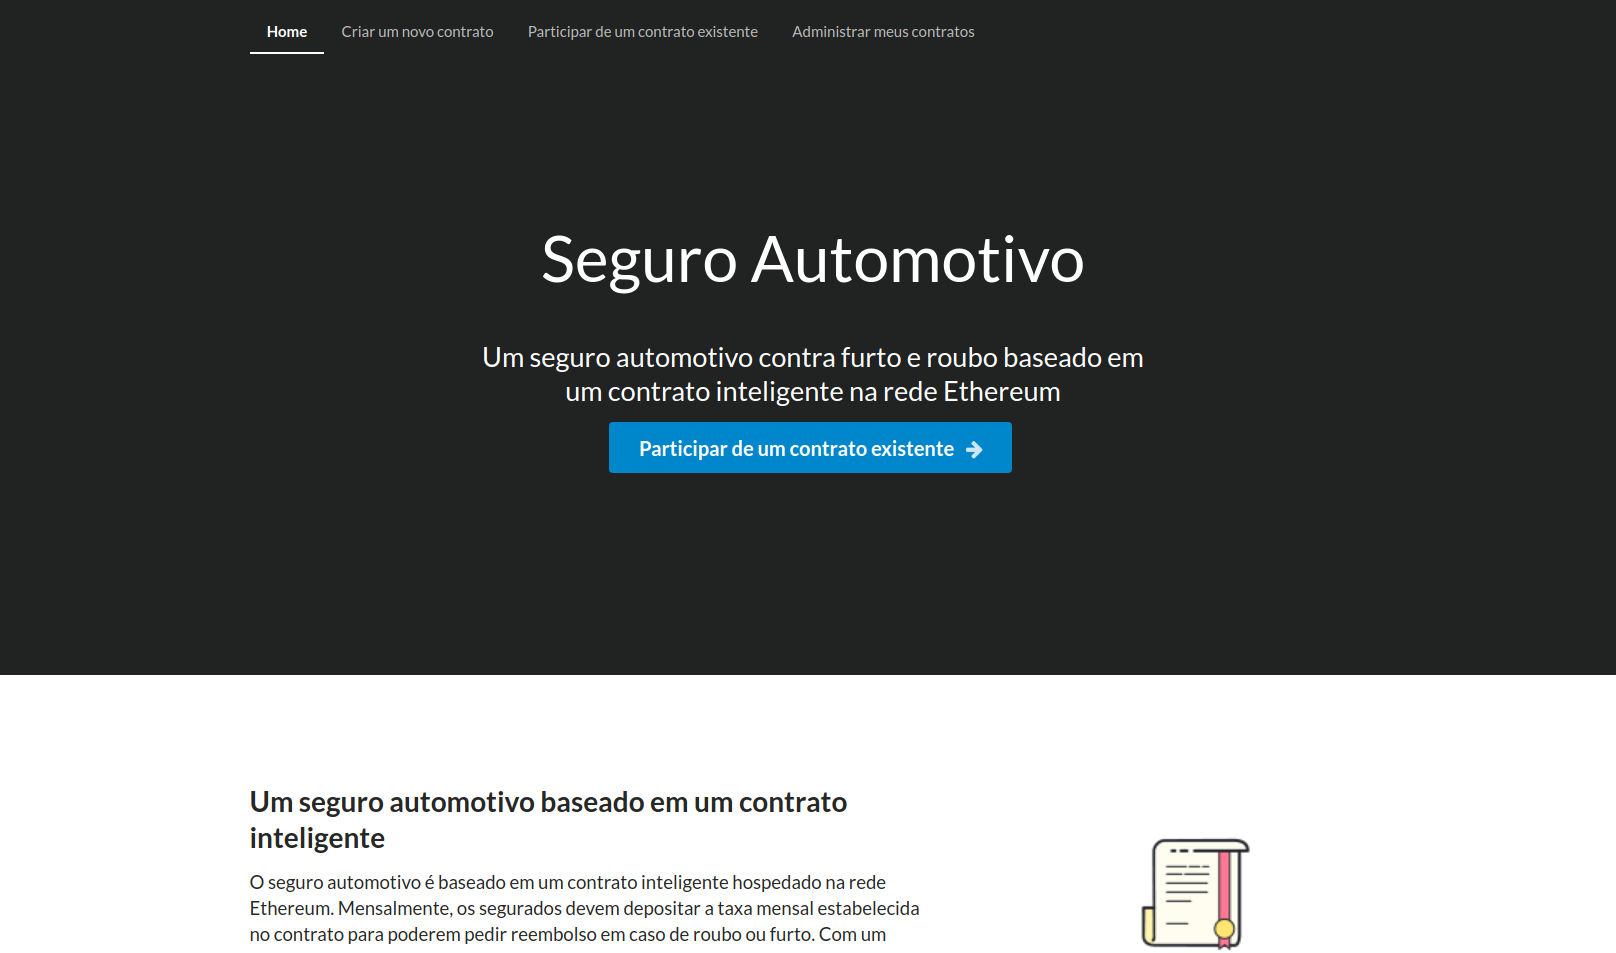
\includegraphics[width=0.9\textwidth]{Cap2/home_page.png}
\caption{Home page da aplicação.}
\label{home_page}
\end{figure}

\begin{figure}[h!]
\centering
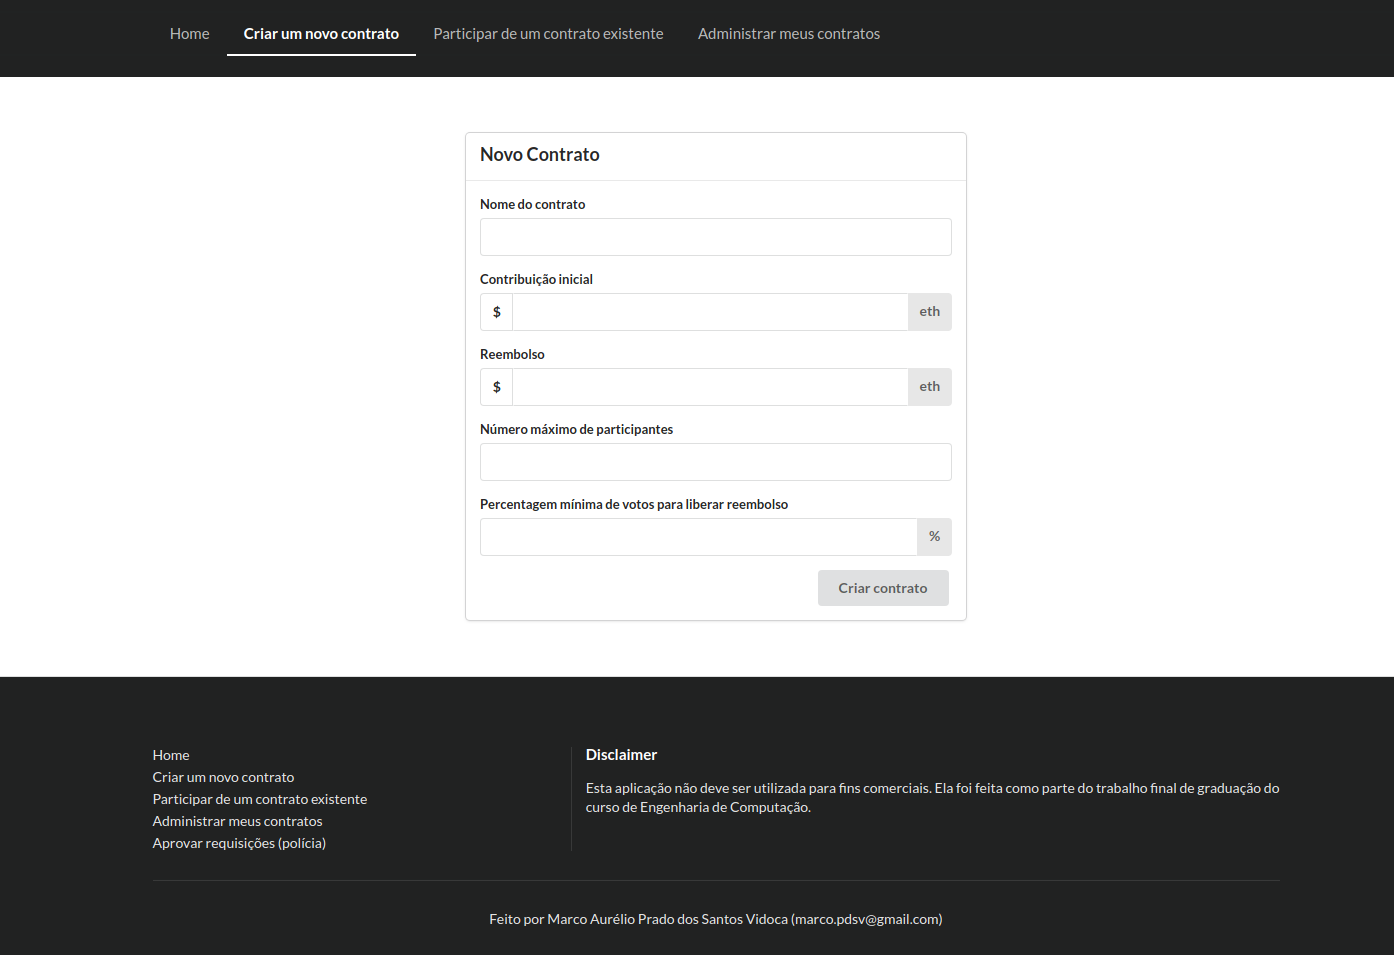
\includegraphics[width=0.9\textwidth]{Cap2/new_contract.png}
\caption{Formulário para a criação de um novo contrato de seguro automotivo.}
\label{new_contract}
\end{figure}

\begin{figure}[h!]
\centering
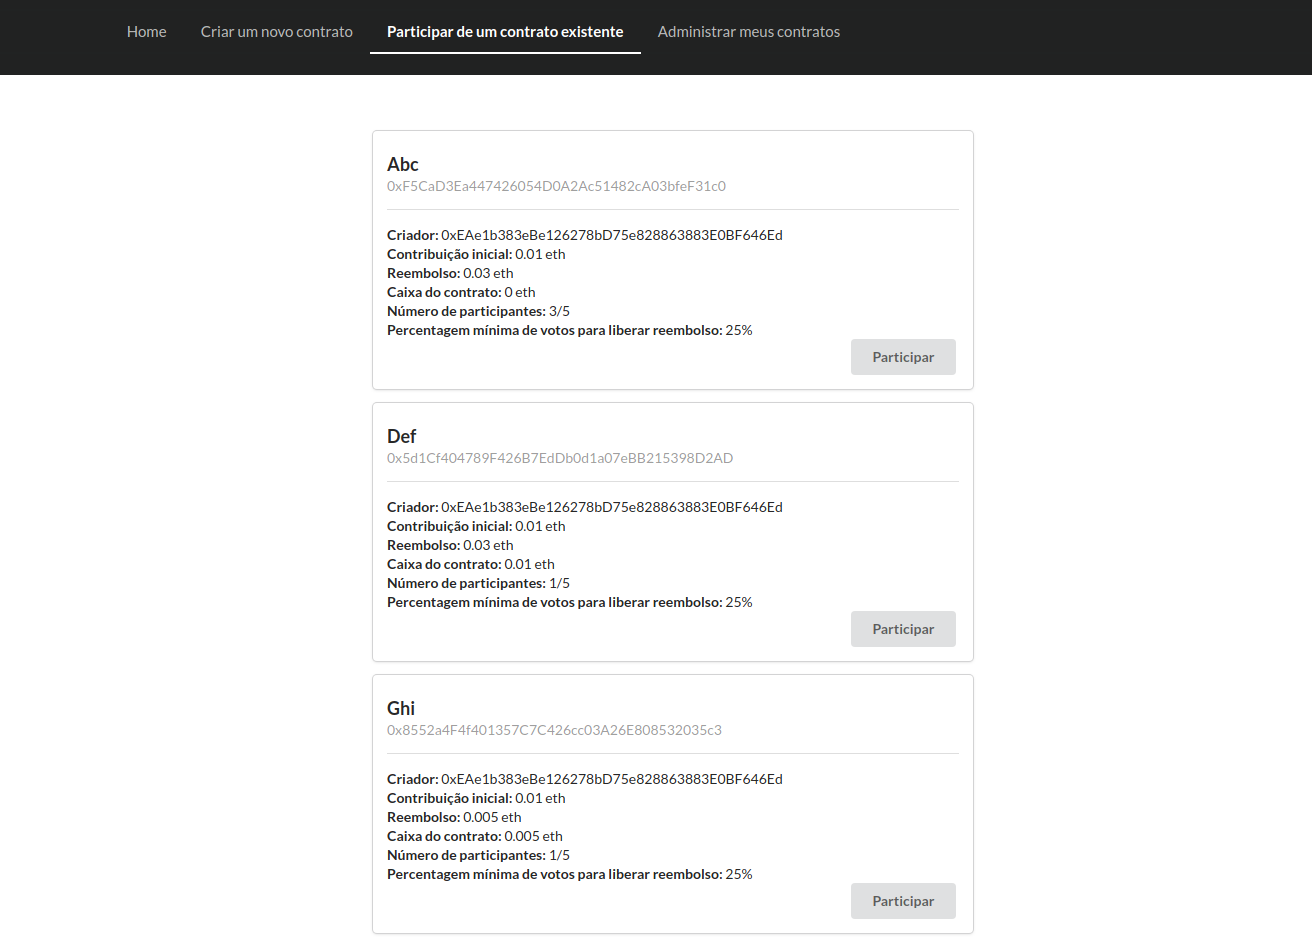
\includegraphics[width=0.9\textwidth]{Cap2/participate_existent_contract.png}
\caption{Lista com os contratos criados e os quais qualquer pessoa pode participar mediante ao pagamento de taxa.}
\label{participate_existent_contract}
\end{figure}

\begin{figure}[h!]
\centering
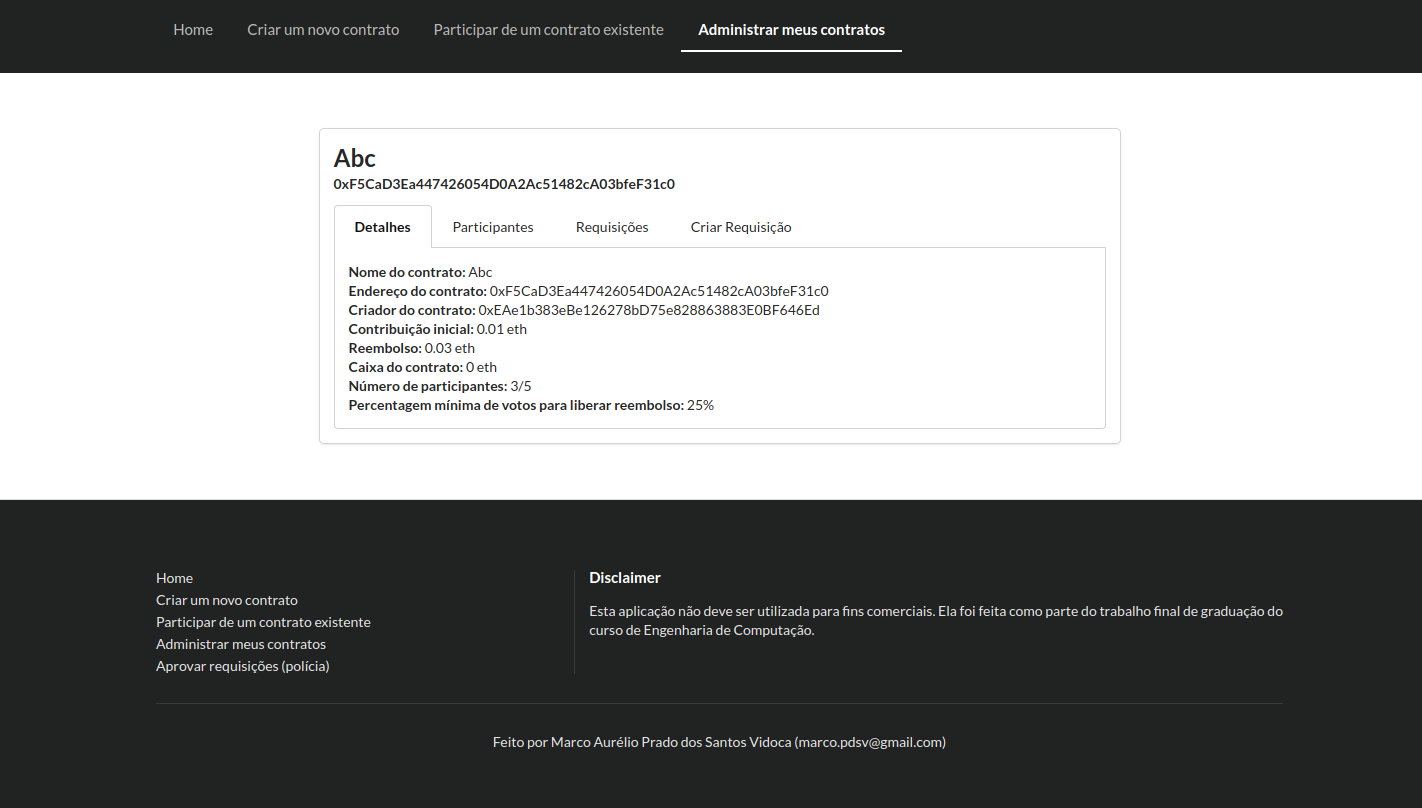
\includegraphics[width=0.9\textwidth]{Cap2/my_contracts_details.png}
\caption{Página contendo os contratos ativos da pessoa que está acessando a aplicação. Nesse caso, se vê a aba de detalhes do contrato.}
\label{my_contracts_details}
\end{figure}

\begin{figure}[h!]
\centering
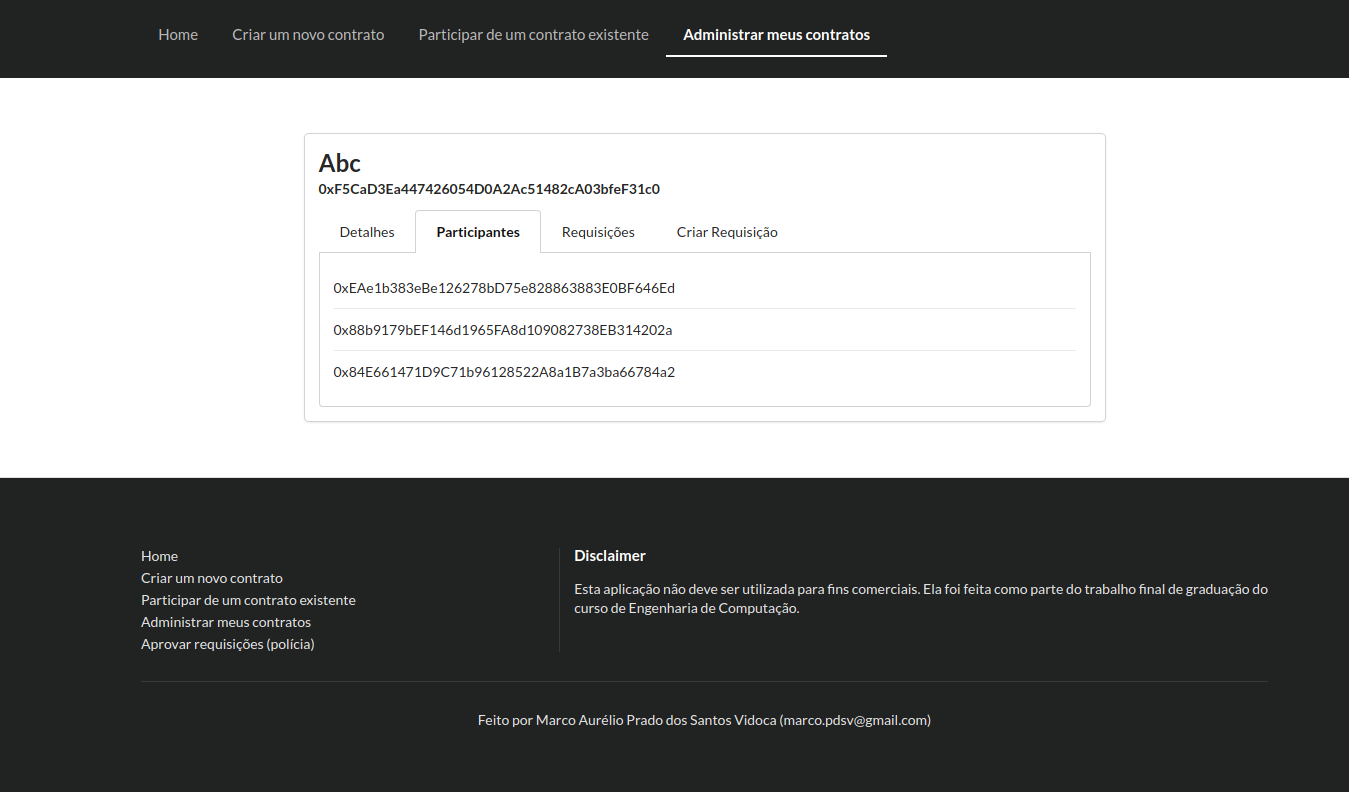
\includegraphics[width=0.9\textwidth]{Cap2/my_contracts_participants.png}
\caption{Página contendo os contratos ativos da pessoa que está acessando a aplicação. Nesse caso, se vê a aba que exibe o endereço da conta Ethereum de quem participa do contrato.}
\label{my_contracts_participants}
\end{figure}

\begin{figure}[h!]
\centering
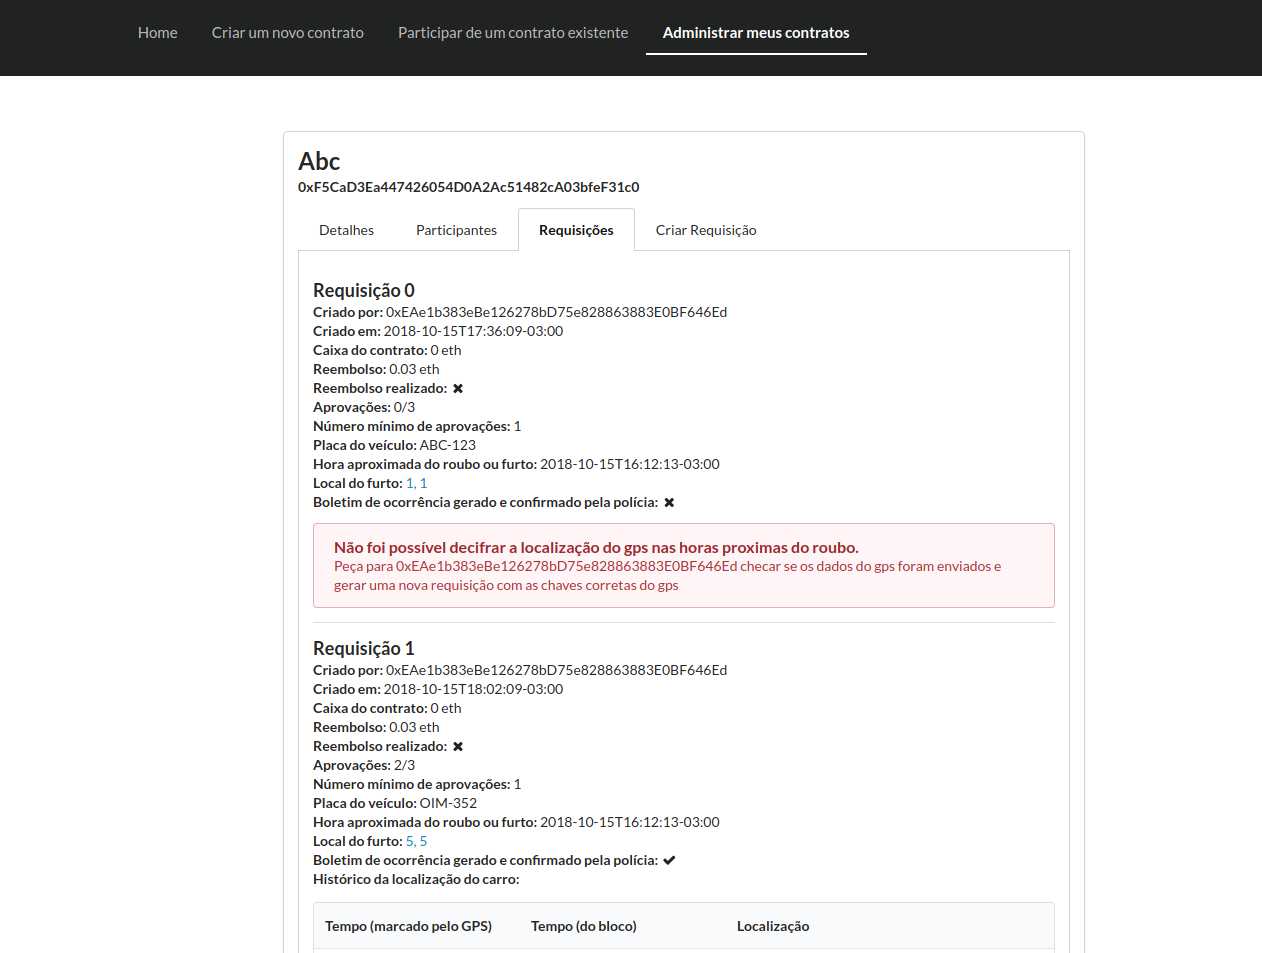
\includegraphics[width=0.9\textwidth]{Cap2/my_contracts_requests.png}
\caption{Página contendo os contratos ativos da pessoa que está acessando a aplicação. Nesse caso, se vê a aba que exibe as requisições de reembolso feitas pelos participantes do contrato.}
\label{my_contracts_requests}
\end{figure}

\begin{figure}[h!]
\centering
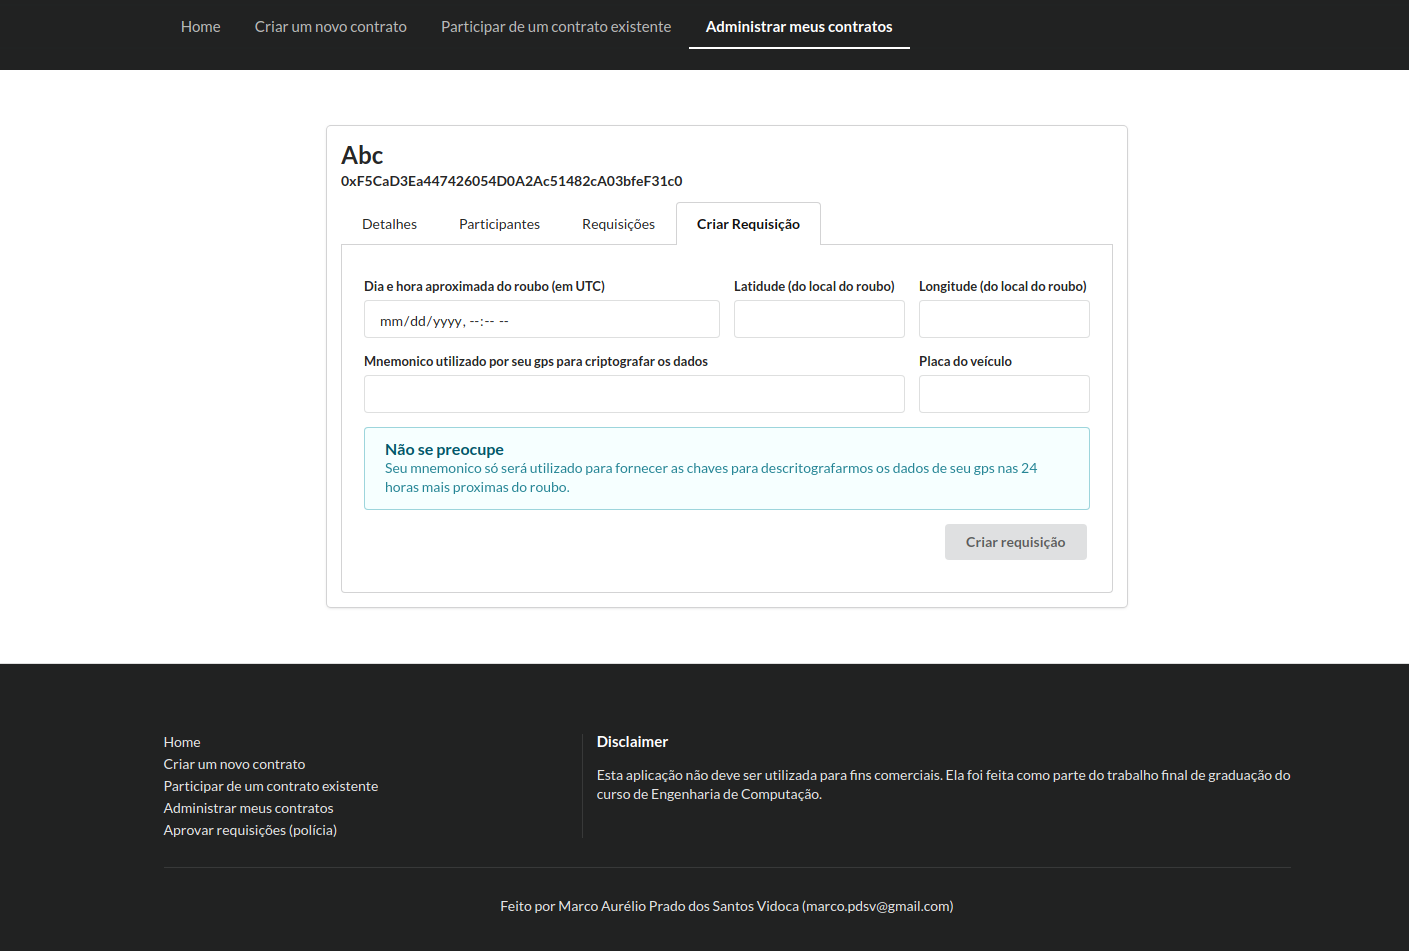
\includegraphics[width=0.9\textwidth]{Cap2/my_contracts_new_request.png}
\caption{Página contendo os contratos ativos da pessoa que está acessando a aplicação. Nesse caso, se vê a aba na qual o participante do contrato pode criar uma nova requisição de reembolso.}
\label{my_contracts_new_request}
\end{figure}

\begin{figure}[h!]
\centering
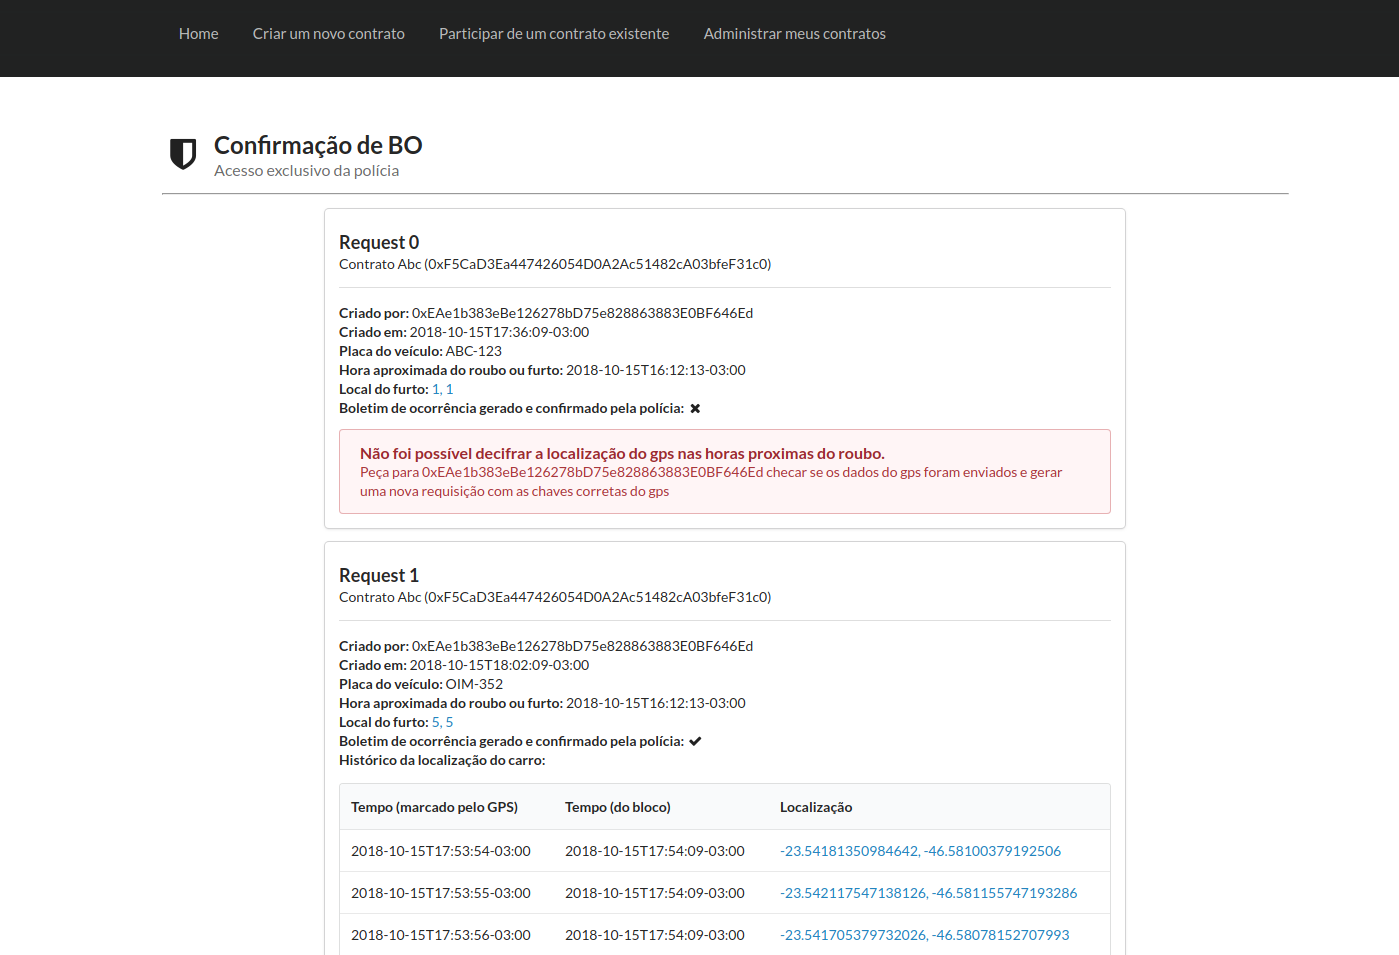
\includegraphics[width=0.9\textwidth]{Cap2/confirm_bo.png}
\caption{Página na qual são exibidos as requisições de reembolso e na qual, apenas a conta Ethereum administrada pela polícia pode aprovar se um boletim de ocorrência condizente com a requisição em questão foi registrado.}
\label{confirm_bo}
\end{figure}

\clearpage
\subsubsection{Comunicação com a Rede Ethereum por meio da lib web3js}

Para a aplicação cliente se comunicar com a rede Ethereum, é utilizada a bliblioteca javascript web3js versão 1.0.0-beta36. Essa biblioteca permite a interação com um nó remoto ou local da rede Ethereum. No código abaixo, pode-se ver como a biblioteca é utilizada na criação de um novo contrato de seguro automotivo:

\begin{code}
\begin{minted}[
frame=lines,
fontsize=\footnotesize,
linenos
]{javascript}
// Importando a lib web3js
import Web3 from 'web3'; 
// Importando o json com as especificações de SmartCarInsuranceContractFactory
import SmartCarInsuranceContractFactory from 
'./build/SmartCarInsuranceContractFactory.json';

// Criando a instância da lib web3 a partir do provedor  do MetaMask
const web3 = new Web3(window.web3.currentProvider);
// Criando uma instância da fábrica de contratos
const smartCarInsuranceContractFactory = new web3.eth.Contract(
    JSON.parse(SmartCarInsuranceContractFactory.interface),
    "0xB7CbfB9d3a64983623f06C410489eA0bCb628B06"
);
// Obtendo as contas cadastradas no MetaMask
const accounts = await web3.eth.getAccounts();

// Chamando o método que cria um novo contrato automotivo, passando
// os parâmetros necessários: nome do contrato, contribuição inicial,
// valor do reembolso, número máximo de participantes e mínima
// percentagem de votos para liberar reembolso
await smartCarInsuranceContractFactory.methods
	.createSmartCarInsuranceContract(
		this.state.contractName,
      	web3.utils.toWei(this.state.initialContribution),
      	web3.utils.toWei(this.state.refundValue),
      	this.state.nMaxParticipants,
      	this.state.minVotePercentageToRefund)
  	.send({
  		from: accounts[0]
	});
\end{minted}
\caption{Biblioteca web3js}
\label{lst:lib_web3js}
\end{code}

Conforme se observa no código acima, o construtor de Web3 recebe window.web3.currentProvider. Para se criar uma instância de um objeto Web3, deve-se passar para o construtor de Web3 um objeto que implemente a interface Provider. Tal objeto é responsável por estabelecer como a lib Web3 irá interagir com o blockchain.

\begin{figure}[h]
\centering
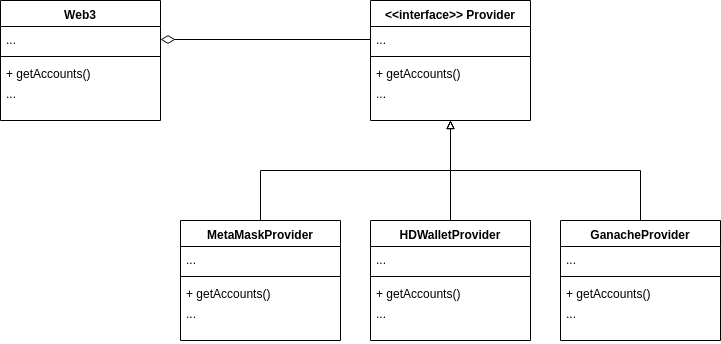
\includegraphics[width=0.7\textwidth]{Cap2/providers.png}
\caption{Strategy pattern com os Providers do Web3.}
\label{providers}
\end{figure}

Na aplicação construída, utilizou-se 3 Providers diferentes:

\begin{itemize}
\item \textbf{MetaMaskProvider:} Metamask é uma extensão do chrome que gerencia as contas dos usuários na rede Ethereum. Ele injeta em toda página web que o usuário visita um Provider com as contas cadastradas pelo usuário e que se comunica com a rede Ethereum utilizando o Infura.
\item \textbf{HDWalletProvider:} Esse provider é utilizado para fazer o deploy de SmartCarInsuranceContractFactory e também na aplicação que simula o gps e envia os dados para o contrato de seuguro automotivo. Esse provider recebe as credenciais da conta Ethereum e a url de accesso do Infura.
\item \textbf{GanacheProvider:} Esse provider é utilizado nos testes dos contratos. O Ganache cria uma rede blockchain Ethereum na máquina local e disponibiliza um provider para se comunicar com rede criada. O Ganache configura tal rede de forma que as transações ocorram rapidamente, criando uma ambiente ideal para testar os contratos antes de fazer o deploy para a rede Ethereum principal.
\end{itemize}

\subsection{Dispositivo GPS}

O dispositivo GPS foi simulado por um código desenvolvido em NodeJs e se encontra disponível no GitHub (\href{https://github.com/marcoprado17/scife-gps-simulator}{https://github.com/marcoprado17/scife-gps-simulator}). O código do simulador foi dividido em dois scripts, o primeiro deles, run.js, é responsável por criar n processos que executam o segundo script, run\_for\_user.js. Esse segundo script, representa o dispositivo GPS de um usuário do sistema e fica constantemente gerando uma latitude e longitude aleatórios a partir de um ponto inicial (figura \ref{gps_location_generator}) para enviar para o contrato após criptografá-los. Seguem abaixo o pseudo código explicando o funcionamento do simulador do dispositivo GPS de um usuário, bem como o código comentado dos principais arquivos:

\begin{enumerate}
\item Obtenção da chave mestre do dispositivo GPS a partir do mnêmonico utilizando o BIP39;
\item Geração inicial da posição do carro, obtendo a latitude a partir de uma distribuição aleatória uniforme entre -23.603244 e -23.504324 e uma longitude a partir de uma distribuição aleatória uniforme entre -46.679381 e -46.561788;
\item Geração de \(\Delta_{lat}\) e \(\Delta_{long}\) a partir de uma distribuição aleatória uniforme entre -0.005 e 0.005;
\item Obtenção das latitudes e longitudes da iteração atual, \(curr_{lat} = curr+{lat} + \Delta_{lat}\) e \(curr_{long} = curr_{long} + \Delta_{long}\);
\item Obtenção Unix Timestamp atual em segundos, \(t_{0}\);
\item Obtenção do índice da chave privada filha a partir da chave privada mestre, \(i = t_{0} - 946684800\). 946684800 representa o Unix Timestamp de 01/01/2000 00:00:00Z. Como a chave mestra pode dar origem a \(2^{32}\) chaves filhas, podemos gerar as chaves privadas que encriptam o dado do sinal GPS até o Unix Timestamp \(t_{1} = 946684800 + 2^{32} = 5241652096\), ou seja, até 02/07/2136 06:28:00Z;
\item Obtenção da chave privada \(k_{priv}\) = i-essima chave filha da chave privada mestre;
\item Encriptação da latitude e longitude do sinal GPS utilizando \(k_{priv}\) e AES256 \cite{aes}.
\item Envio do sinal GPS para o contrato na rede Ethereum;
\item Medição dos dados pertinentes ao envio dessa amostra de sinal GPS para posterior análise.
\end{enumerate}

\begin{figure}[h!]
\centering
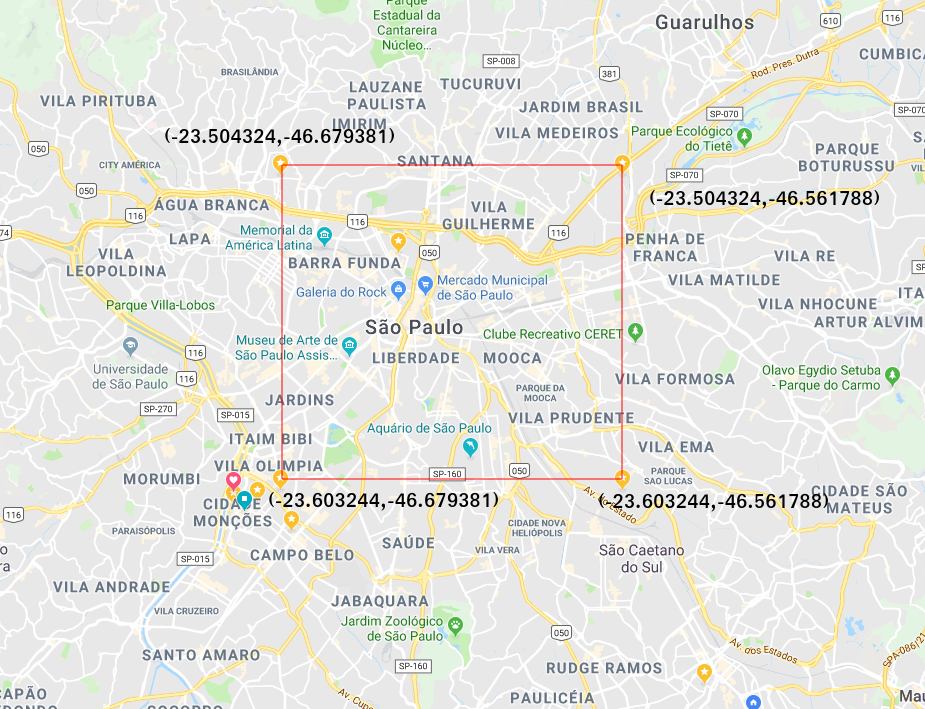
\includegraphics[width=0.9\textwidth]{Cap2/gps_location_generator}
\caption{Posição inicial do sinal GPS do carro de um usuário.}
\label{gps_location_generator}
\end{figure}

\clearpage
\begin{code}
\begin{minted}[
frame=lines,
fontsize=\footnotesize,
linenos
]{javascript}
const spawn = require('child_process').spawn;
// Obtendo o arquivo de configurações
const configs = require('./configs');

[...Array(configs.nUsers).keys()].map(user_idx => {
    // Iniciando um processo que executa o script run_for_user.js
    let command = spawn("node", ["run_for_user.js", user_idx]);
    
    // Imprimindo o stout dos processos filhos no processo mãe
    command.stdout.on('data', function (data) {
        process.stdout.write(data.toString());
    });
    
    // Imprimindo o stderr dos processos filhos no processo mãe
    command.stderr.on('data', function (data) {
        console.log("*** STDERR ***");
        process.stdout.write(data.toString());
    });
    
    // Imprimindo no processo mãe, os processos filhos que finalizaram
    command.on('exit', function (code) {
        console.log('child process exited with code ' + code.toString());
    });
});
\end{minted}
\caption{Script run.js}
\label{lst:run_script}
\end{code}

\clearpage
\begin{code}
\begin{minted}[
frame=lines,
fontsize=\footnotesize,
linenos
]{javascript}
// Obtenção das dependências
const Web3 = require('web3');
const secrets = require('./secrets');
const HDWalletProvider = require('truffle-hdwallet-provider');
const SmartCarInsuranceContract = 
require('./ethereum/build/SmartCarInsuranceContract.json');
const configs = require('./configs');
const Tx = require('ethereumjs-tx');
const bip39 = require("bip39");
const hdkey = require('ethereumjs-wallet/hdkey');
const crypto = require('crypto');
const fs = require('fs');

// Obtenção do indice que representa esse usuário
const user_idx = parseInt(process.argv[2]);

// Obtenção do Provider que será utilizado pela lib web3js para 
// comunicação com o nó Ethereum remoto por meio do Infura
const provider = new HDWalletProvider(
    secrets.mnemonic,
    secrets.infuraUrl,
    user_idx
);

const privKeyBuffer = provider.wallet._privKey;
const accountAddress = provider.address;
const web3 = new Web3(provider);
// Obtenção do contrato
const smartCarInsuranceContract = 
new web3.eth.Contract(
    JSON.parse(SmartCarInsuranceContract.interface), configs.contractAddress);

let nTransactions = 0;

// Obtenção da latitude e longitude inicial
let currentLat = configs.minInitialLat + 
    (configs.maxInitialLat-configs.minInitialLat)*Math.random();
let currentLong = configs.minInitialLong + 
    (configs.maxInitialLong-configs.minInitialLong)*Math.random();

// Obtenção da Hierarchical Deterministic wallet a partir do 
// mnemônico que gerará a seed
const masterSeed = bip39.mnemonicToSeed(secrets.gpsMnemonic);
const gpsHdwallet = hdkey.fromMasterSeed(masterSeed);

// Configurações iniciais do objeto que representa o relatório
let report = {};
report.configs = configs;
report.data = [];

let initialNonce = 0;

// Função que converte uma array de bytes para uma string em hexadecimal 
let decodeHexStringToByteArray = function(hexString) {
    // console.log(hexString);
    var result = [];
    while (hexString.length >= 2) { 
        result.push(parseInt(hexString.substring(0, 2), 16));
        hexString = hexString.substring(2, hexString.length);
    }
    // console.log(result);
    return result;
};

(async function(){
    initialNonce = await web3.eth.getTransactionCount(accountAddress);

    console.log(`initialNonce: ${initialNonce}`);

    // Aguardando certo intervalo de tempo para começar a enviar 
    //os dados do gps
    setTimeout(() => {
    // Enviando os dados do GPS a cada 
    // configs.sendLocationPeriodInMiliseconds milisegundos
    setInterval(async () => {
    try {
        // Incrmentando a transação
        let thisTransaction = nTransactions++;

        // Obtendo o Unix Timestamp atual em segundos
        const currentUnixTimestamp = Math.floor(Date.now()/1000);

        // Obtendo a latitude e longitude dessa iteração
        latLongData = {
            lat: currentLat,
            long: currentLong
        }

        // Setando a latitude e longitude da próxima iteração
        currentLat += (Math.random() > 0.5 ? 1 : -1)*
        Math.random()*configs.maxCoordinateDeltaBetweenCalls;
        currentLong += (Math.random() > 0.5 ? 1 : -1)*
        Math.random()*configs.maxCoordinateDeltaBetweenCalls;

        let thisLat = currentLat;
        let thisLong = currentLong;

        // Obtendo o indice da chave privada filha que será 
        // utilizada para encriptar o sinal GPS dessa iteração
        const i = currentUnixTimestamp-946684800;
        const key = gpsHdwallet
        .deriveChild(i).getWallet().getPrivateKey();

        // Encriptando os dados do GPS com AES256
        const cipher = crypto.createCipher("aes256", key)
        let encryptedGpsData = cipher.update(
            JSON.stringify(latLongData),'utf8','hex'
        );
        encryptedGpsData += cipher.final('hex');

        // Obtendo os dados da transação Ethereum que será 
        // utilizado para chamar a função do nosso contrato 
        // que recebe o sinal GPS
        const data = smartCarInsuranceContract.methods
            .pushGpsData(currentUnixTimestamp, encryptedGpsData)
            .encodeABI();
        let dataAsByteArray = decodeHexStringToByteArray(
            data.substr(2)
        );
        let nNonZeroBytes = 0;
        let nZeroBytes = 0;
        dataAsByteArray.map((byte) => {
            if(byte == 0){
                nZeroBytes++;
            }
            else{
                nNonZeroBytes++;
            }
        });
        // console.log(`nZeroBytes: ${nZeroBytes}`);
        // console.log(`nNonZeroBytes: ${nNonZeroBytes}`);

        const nonce = initialNonce + thisTransaction;

        // Setando os dados da transação
        const txData = {
            nonce: web3.utils.toHex(nonce),
            gasLimit: web3.utils.toHex(1000000),
            gasPrice: web3.utils.toHex(1e9), // 1 Gwei
            to: configs.contractAddress,
            from: accountAddress,
            data: data
        };

        // console.log(txData);

        // Assinando a transação com a chave privada
        const transaction = new Tx(txData);
        transaction.sign(privKeyBuffer);
        const serializedTx = transaction.serialize().toString('hex');
        const sendTxUnixTimestamp = Math.floor(Date.now()/1000);
        web3.eth.sendSignedTransaction('0x' + serializedTx)
            .once('transactionHash', function(hash) {
                console.log(hash);
            })
            .on('error', function(err) {
                // Adicionando os dados dessa transação mal 
                // sucedida ao relatório

                let msg = "";
                msg += `Sending transaction ${thisTransaction}/${nonce} 
                for user ${user_idx} (${accountAddress}) at 
                ${currentUnixTimestamp}\n`;
                msg += `ERROR: ${err.message}`;
                console.log(msg);

                const finishTxUnixTimestamp = Math.floor(Date.now()/1000);
                report.data.push({
                    idx: thisTransaction,
                    status: "ERROR",
                    message: err.message,
                    creationUnixTimestamp: currentUnixTimestamp,
                    lat: thisLat,
                    long: thisLong,
                    encryptedGpsData: encryptedGpsData,
                    sendTxUnixTimestamp: sendTxUnixTimestamp,
                    finishTxUnixTimestamp: finishTxUnixTimestamp,
                    latency: (finishTxUnixTimestamp-sendTxUnixTimestamp),
                    txData: txData,
                    nNonZeroBytes: nNonZeroBytes,
                    nZeroBytes: nZeroBytes
                });
            })
            .then(function(result) {
                // Adicionando os dados dessa transação bem 
                // sucedida ao relatório

                let msg = "";
                msg += `Sending transaction ${thisTransaction}/${nonce} 
                for user ${user_idx} (${accountAddress}) at 
                ${currentUnixTimestamp}\n`;
                msg += `SUCCESS:\n`;
                msg += `${JSON.stringify(result, null, 4)}`;
                console.log(msg);

                const finishTxUnixTimestamp = Math.floor(Date.now()/1000);
                report.data.push({
                    idx: thisTransaction,
                    status: "OK",
                    creationUnixTimestamp: currentUnixTimestamp,
                    lat: thisLat,
                    long: thisLong,
                    encryptedGpsData: encryptedGpsData,
                    sendTxUnixTimestamp: sendTxUnixTimestamp,
                    finishTxUnixTimestamp: finishTxUnixTimestamp,
                    latency: (finishTxUnixTimestamp-sendTxUnixTimestamp),
                    txData: txData,
                    result: result,
                    nNonZeroBytes: nNonZeroBytes,
                    nZeroBytes: nZeroBytes
                });
            });
    }
    catch(err){
        console.error(err);
    }
    }, configs.sendLocationPeriodInMiliseconds);
    }, Math.random() * configs.sendLocationPeriodInMiliseconds);
}());

// Enviando para um arquivo .json os dados do relatório 
// a cada 15 segundos
setInterval(function(){
    const currentUnixTimestamp = Math.floor(Date.now()/1000);
    console.log(`Saving report (${currentUnixTimestamp}.json)...`);
    let stringfiedReport = JSON.stringify(report, null, '\t');
    console.log("report.data.length", report.data.length);
    console.log("Report stringfied");
    // console.log(stringfiedReport);
    fs.writeFileSync(
        `./temp_reports/${currentUnixTimestamp}.json`, 
        stringfiedReport, 'utf-8'
    );
    console.log(`Report ${currentUnixTimestamp}.json saved`);
}, 15000);
\end{minted}
\caption{Script run\_for\_user.js}
\label{lst:run_for_user_script}
\end{code}

\section{Construção do seguro automotivo utilizando a arquitetura híbrida}

\begin{figure}[h]
\centering
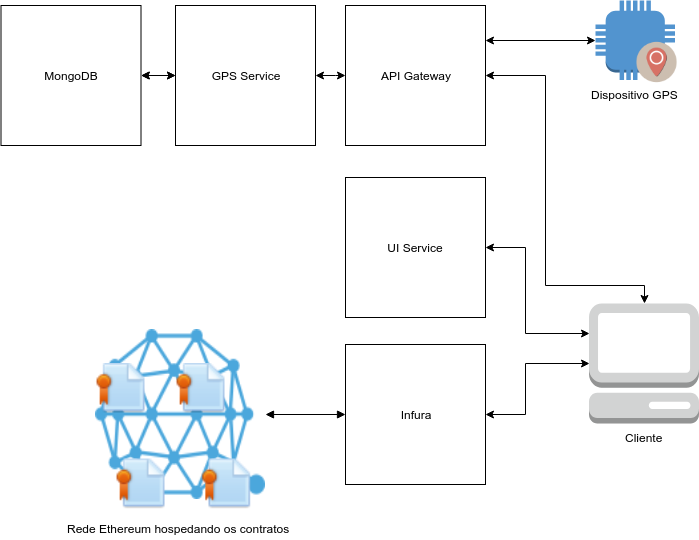
\includegraphics[width=0.9\textwidth]{Cap2/architecture_hybrid.png}
\caption{Arquitetura híbrida.}
\label{architecture_hybrid}
\end{figure}

Como pode-se observar na figura \ref{architecture_hybrid}, essa arquitetura é composta por 8 componentes:

\begin{itemize}
	\item \textbf{Cliente:} O cliente representa a aplicação web que os usuários do seguro utilizam para interagirem com os contratos e com o GPS Service. Devido a semelhança que tal aplicação possue com o cliente da arquitetura 100\% Ethereum e devido ao fato de aplicação cliente não ser necessária para análise proposta, tal componente não foi desenvolvido;
    \item \textbf{Servidor de UI:} É o servidor de recursos estáticos que provê o arquivo javascript que contém o código do cliente, bem como as imagens da aplicação web;
    \item \textbf{Infura:} Infura (\href{https://infura.io/}{https://infura.io/}) é um serviço web que prove acesso a rede Ethereum por meio de uma API REST. Esse serviço abstrai a complexidade de criar e manter um nó próprio conectado a rede Ethereum;
    \item \textbf{Rede Ethereum:} Representa a rede Ethereum composta por nós espalhados pelo mundo todo;
    \item \textbf{Contratos:} Representa os contratos de seguro automotivo criados e mantidos pelos usuários da aplicação. Os contratos dessa arquitetura são semelhantes aos contratos da arquitetura 100\% Ethereum, a diferença é que não possuiriam a função que recebe os dados do GPS e nem a estrutura de dados que armazena os dados do GPS. Devido a tal semelhança, os contratos para a arquitetura híbrida não foram desenvolvidos;
    \item \textbf{Dispositivo GPS:} O dispositivo GPS é responsável por enviar constantemente a localização do carro dos participantes do contrato de seguro automotivo para o GPS Service. Para manter a privacidade dos usuários, o envio da latitude e longitude é criptografado. O código que simula o dispositivo GPS está disponível no GitHub (\href{https://github.com/marcoprado17/scih-gps-simulator}{https://github.com/marcoprado17/scih-gps-simulator}). A única diferença em relação ao simulador de GPS da arquitetura 100\% Ethereum é o envio dos dados do GPS para o API Gateway com uma requisição http do tipo POST, como pode ser visto no código \ref{scih_gps_sim_diff};
    \item \textbf{API Gateway:} Serviço responsável por verificar a autenticidade dos dados enviados pelos dispositivo GPS. Esse serviço também é responsável por direcionar os dados do GPS para o GPS Service. O Código completo desse serviço está disponível no GitHub (\href{https://github.com/marcoprado17/scih-api-gateway}{https://github.com/marcoprado17/scih-api-gateway});
    \item \textbf{GPS Service:} Serviço responsável por interagir com o banco de dados MongoDB para armazenamento dos dados do GPS. O Código completo desse serviço está disponível no GitHub (\href{https://github.com/marcoprado17/scih-gps-service}{https://github.com/marcoprado17/scih-gps-service});
    \item \textbf{MongoDB:} Banco de dados MongoDB versão 3.6.2.
\end{itemize}

\clearpage
\begin{code}
\begin{minted}[
frame=lines,
fontsize=\footnotesize,
linenos
]{javascript}
axios.post(`http://35.239.45.68:81/api/accounts/${accountAddress}/
	contracts/${configs.contractAddress}/gps-data`, {
  data,
  v,
  r,
  s,
  from: accountAddress
})
\end{minted}
\caption{Envio dos dados do GPS para o API Gateway com o uso da biblioteca axios do nodejs}
\label{lst:scih_gps_sim_diff}
\end{code}

	Nas próximas seções será detalhado a implementação dos principais componentes do sistema: API Gateway e GPS Service.

\subsection{Implementação comentada do API Gateway}

\begin{code}
\begin{minted}[
frame=lines,
fontsize=\footnotesize,
linenos
]{javascript}
// Obtenção das dependências
var express = require('express');
var router = express.Router();
const httpProxy = require('express-http-proxy');
const { body, param, validationResult } = require('express-validator/check');
var nconf = require('nconf');
const ethereumjs = require('ethereumjs-util');
const wrapAsync = require('./wrap-assync');
const assert = require('assert');

// Returning 200 on / to serve as health check to ingress
// https://cloud.google.com/kubernetes-engine/docs/tutorials/http-balancer#remarks
router.get('/', function(req, res, next) {
  res.sendStatus(200)
});

/* GET home page. */
router.get('/api', function(req, res, next) {
  res.send("Home page da api!!!");
});

/* gps-service rules */
const gpsServiceProxy = httpProxy(nconf.get("gpsServiceHost"));

router.post('/api/accounts/:accountId/contracts/:contractId/gps-data', [
  // Validando o corpo do request
  body("data.encryptedGpsData").isString(),
  body("data.creationUnixTimestamp").isNumeric(),
  body("from").isString(),
  body("v").isNumeric(),
  body("r.type").equals("Buffer"),
  body("r.data").isArray(),
  body("r.data.*").isNumeric(),
  body("s.type").equals("Buffer"),
  body("s.data").isArray(),
  body("s.data.*").isNumeric(),
  param("accountId").isString(),
  param("contractId").isString()
], wrapAsync(async (req, res, next) => {
    // Se ocorreu algum erro de validação, será retornado o código http 400
    const errors = validationResult(req);
    if (!errors.isEmpty()) {
      return res.status(400).json({ errors: errors.array() });
    }

    // Validando a assinatura ECDSA
    let dataHash = await ethereumjs.sha3(JSON.stringify(req.body.data));
    
    let r = new Buffer(req.body.r.data);
    let s = new Buffer(req.body.s.data);

    try {
      const validSign = ethereumjs.isValidSignature(req.body.v, r, s);
      const pubKey  = ethereumjs.ecrecover(
        ethereumjs.toBuffer(dataHash), req.body.v, r, s);
      const addrBuf = ethereumjs.pubToAddress(pubKey);
      const addr    = ethereumjs.bufferToHex(addrBuf);
      assert(validSign);
      assert.equal(req.body.from, addr)
    }
    catch(err) {
      // Caso a assinatura seja inválida, será retornado o código http 400
      return res.status(400).json({ error: err.message });
    }
    
    // Enviando o dado para GPS Service
    gpsServiceProxy(req, res, next);
}));

// Rota utilizada para obtenção dos dados do GPS
router.get('/api/accounts/:accountId/contracts/:contractId/gps-data', 
(req, res, next) => {
  gpsServiceProxy(req, res, next);
});

module.exports = router;
\end{minted}
\caption{Principais endpoints do API Gateway}
\label{lst:api_gateway}
\end{code}

\subsection{Implementação comentada do GPS Service}

\begin{code}
\begin{minted}[
frame=lines,
fontsize=\footnotesize,
linenos
]{javascript}
const mongoose = require('mongoose');
const timestamps = require('mongoose-timestamp');

const GpsDataSchema = new mongoose.Schema({
    data: {
        // Latitude e longitude encriptada
        encryptedGpsData: { 
            type: String,
            required: true,
        },
        // Unix timestamp de quando essa amostra
        // de sinal GPS foi obtida
        creationUnixTimestamp: {   
            type: Number,
            required: true,
        }
    },
    // Endereço de quem enviou tal dado
    from: {
        type: String,
        require: true
    },
    // Reconver id
    v: {
        type: Number,
        required: true
    },
    // Parâmetro r da assinatura ECDSA
    r: {
        type: Buffer,
        required: true
    },
    // Parâmetro s da assinatura ECDSA
    s: {
        type: Buffer,
        required: true
    },
    // Endereço ethreum da conta que envou tal sinal
    accountId: {
        type: String,
        required: true,
    },
    // Endereço Ethereum do contrato
    contractId: {
        type: String,
        required: true,
    },
}, { collection: 'gpsData' })

GpsDataSchema.plugin(timestamps)

module.exports = exports = mongoose.model('GpsData', GpsDataSchema)
\end{minted}
\caption{Esquema que modela como as informações de uma amostra do sinal GPS será armazenada no banco de dados.}
\label{lst:gps_data_schema}
\end{code}

\begin{code}
\begin{minted}[
frame=lines,
fontsize=\footnotesize,
linenos
]{javascript}
const router = new (require('restify-router')).Router();
const GpsDataSchema = require('./model');

// Endpoint para obtenção dos dados do GPS
router.get('/', function (req, res, next) {
	// default limit to 10 docs
	let limit = parseInt(req.query.limit, 10) || 10; 
	// default skip to 0 docs
	let skip  = parseInt(req.query.skip, 10) || 0; 
	let query = req.params || {};

	// remove skip and limit from data to avoid false querying
	delete query.skip
	delete query.limit

	// Obtendo um determinado dado do GPS
	GpsDataSchema
		.find(query)
		.skip(skip)
		.limit(limit)
		.then(allGpsData => {
			res.send(200, allGpsData)
			next()
		})
		.catch(err => {
			res.send(500, err)
		})
});

// Enviando uma amostra do sinal GPS para o banco de dados
router.post('/', function (req, res, next) {
	// console.log(req.params);
	// Adicionando accountId e contractId ao dado que será 
	// armazenado no banco de dados
	let data = Object.assign({}, 
		{ 	
			accountId: req.params.accountId, 
			contractId: req.params.contractId 
		}, req.body) || {}
	// console.log(data);

	// Enviando para o banco de dados o dado
	GpsDataSchema
		.create(data)
		.then(gpsData => {
			res.send(200)
			next()
		})
		.catch(err => {
			res.send(500, err)
		})
});

module.exports = router;
\end{minted}
\caption{Principais endpoints de GPS Service.}
\label{lst:gps_service_endpoint}
\end{code}










\chapter{Resultados}
\section{Resultados do desempenho do simulador GPS para a arquitetura baseada 100\% na rede Ethereum}

Para testar o desempenho do simulador GPS para a arquitetura baseada 100\% na rede Ethereum, foi realizado um teste simulando um único GPS que enviava ao contrato a latitude e longitude obtida a cada 1 segundo.

\begin{figure}[h!]
\centering
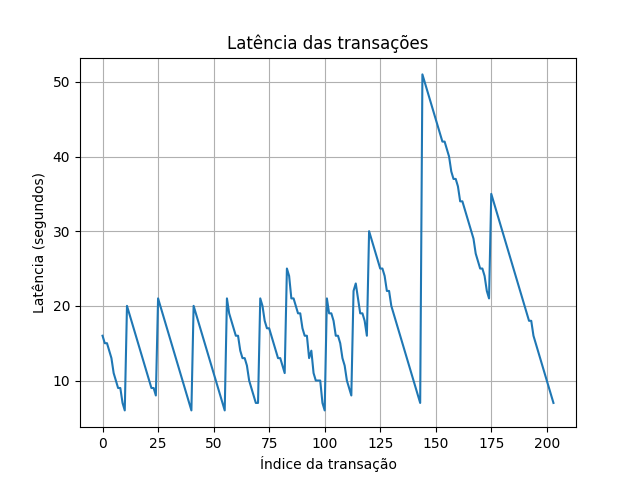
\includegraphics[width=0.7\textwidth]{Cap3/scife_gps_sim_latency.png}
\caption{Latência das transações.}
\label{scife_gps_sim_latency}
\end{figure}

\begin{figure}[h!]
\centering
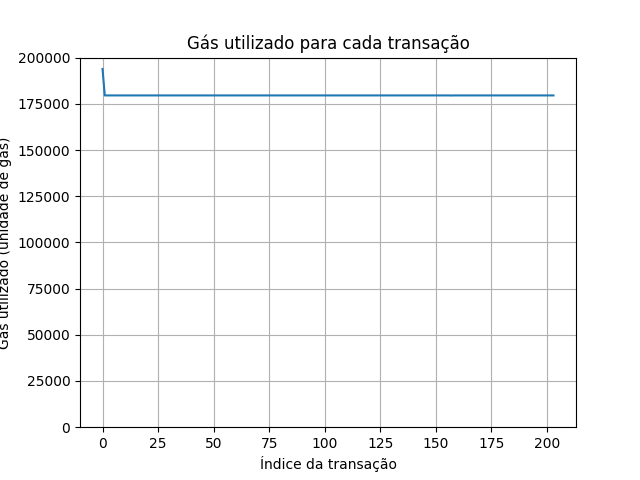
\includegraphics[width=0.7\textwidth]{Cap3/scife_gps_sim_gas_used.png}
\caption{Quantia de gás utilizada por cada transação.}
\label{scife_gps_sim_gas_used}
\end{figure}

\begin{figure}[h!]
\centering
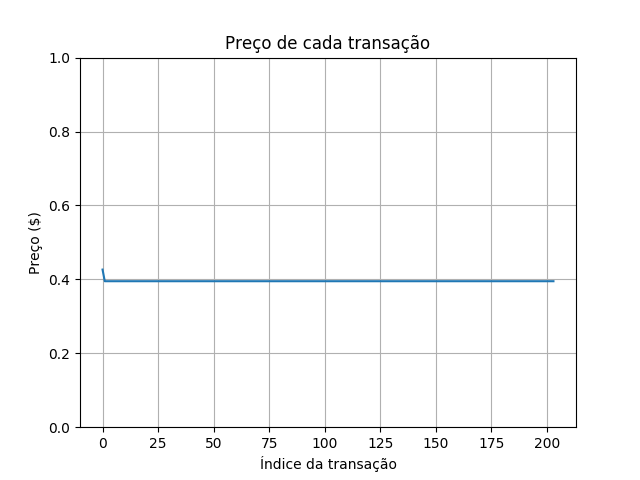
\includegraphics[width=0.7\textwidth]{Cap3/scife_gps_sim_price.png}
\caption{Preço de cada transação}
\label{scife_gps_sim_price}
\end{figure}

Em todos os resultados, para se obter o preço, em dollar, consumido por cada chamada a uma função do contrato, foi considerado que o preço do gás é 10000000000 wei (uma aproximação válida, conforme se vê na figura \ref{gas_price_chart}) e que 1 ETH = \$ 220.00 (uma aproximação válida, conforme se vê na figura \ref{eth_price_chart}).

\begin{figure}[h!]
\centering
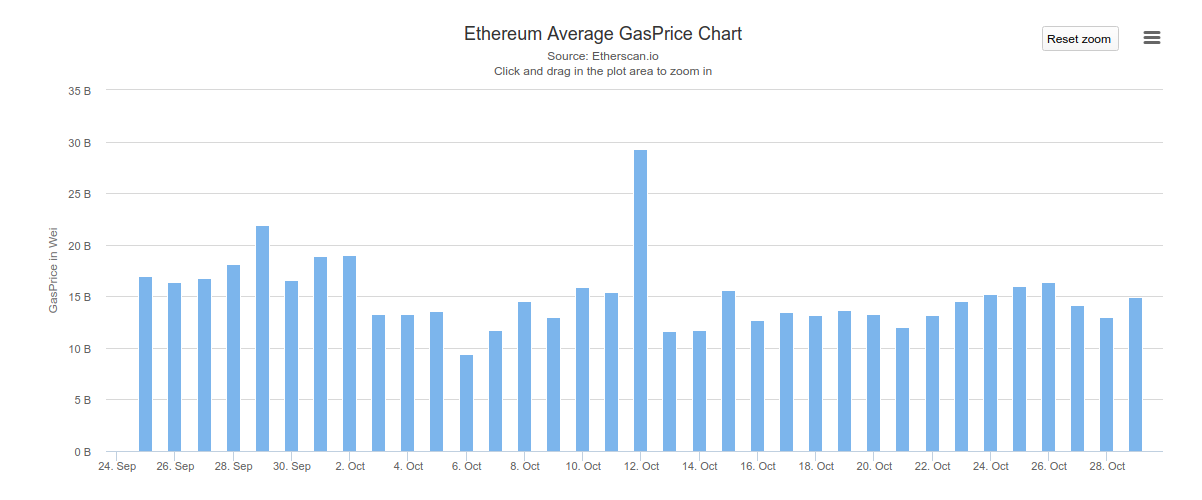
\includegraphics[width=1\textwidth]{Cap3/gas_price_chart}
\caption{Preço dos gás na rede Etherem oficial. Fonte: \href{https://etherscan.io/}{https://etherscan.io/}.}
\label{gas_price_chart}
\end{figure}

\begin{figure}[h!]
\centering
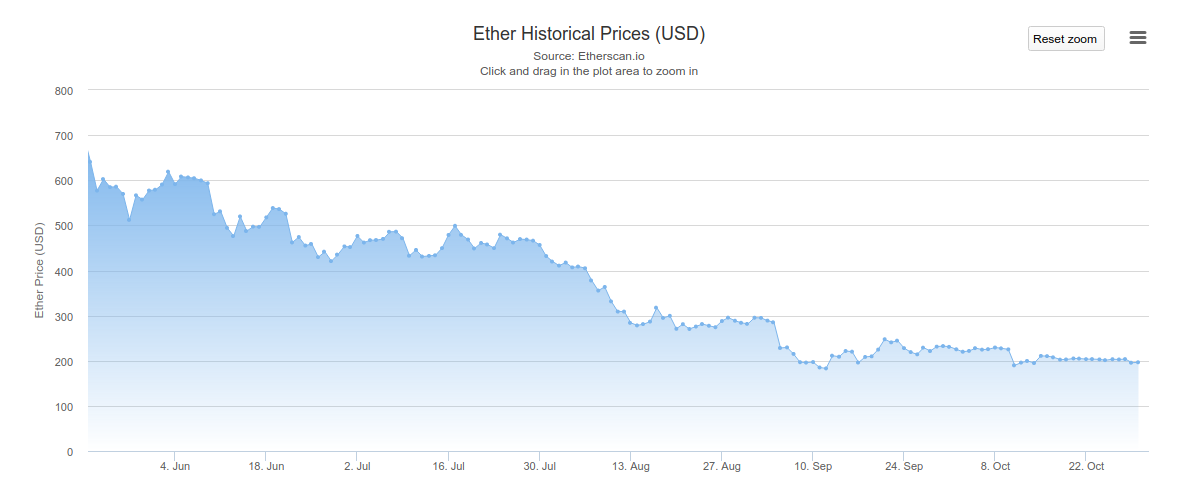
\includegraphics[width=1\textwidth]{Cap3/eth_price_chart}
\caption{Preço do ETH entre Junho e Outubro de 2018. Fonte: \href{https://etherscan.io/}{https://etherscan.io/}.}
\label{eth_price_chart}
\end{figure}

\section{Resultados do desempenho da rede Ethereum para a arquitetura baseada 100\% na rede Ethereum}

Como o contrato está sendo executado nos nós da rede Ethereum, o único valor que nos interessa é a quantia de gás utilizada na chamada de cada uma das funções do contrato. Vale ressaltar que apenas as funções do contrato que modicam os dados internos do contrato consomem gás. As funções que apenas leem os dados internos do contrato (apresentam a palavra chave ``view'' na definição do contrato) não consomem gás. O script que foi utilizado para medir a quantia de gás utilizada por cada função está disponível no GitHub (\href{https://github.com/marcoprado17/scife-calling-all-contract-functions}{https://github.com/marcoprado17/scife-calling-all-contract-functions}).

\begin{table}[h!]
\caption{Quantia de gás consumida por cada uma das funções do contrato.}
\label{my-label}
\begin{center}
\begin{tabular}{cccc}
\hline
Função                   & Parâmetros                                                                         & Gás utilizado & Preço (\$) \\ \hline
enterContract (1º conta) & -                                                                                  & 133043        & 0.2926946  \\ \hline
enterContract (2º conta) & -                                                                                  & 103043        & 0.2266946  \\ \hline
pushGpsData              & \begin{tabular}[c]{@{}c@{}}1540993386,\\ hex string de 64 caracteres\end{tabular}  & 149349        & 0.3285678  \\ \hline
pushGpsData              & \begin{tabular}[c]{@{}c@{}}1540993387,\\ hex string de 64 caracteres\end{tabular}  & 135029        & 0.2970638  \\ \hline
pushGpsData              & \begin{tabular}[c]{@{}c@{}}1540993388,\\ hex string de 128 caracteres\end{tabular} & 179533        & 0.3949726  \\ \hline
pushGpsData              & \begin{tabular}[c]{@{}c@{}}1540993389,\\ hex string de 192 caracteres\end{tabular} & 268541        & 0.5907902  \\ \hline
createNewRefundRequest   & hex string de 64 caracteres                                                        & 164703        & 0.3623466  \\ \hline
createNewRefundRequest   & hex string de 128 caracteres                                                       & 194207        & 0.4272554  \\ \hline
createNewRefundRequest   & hex string de 192 caracteres                                                       & 283215        & 0.623073   \\ \hline
approveRequest           & 0                                                                                  & 66478         & 0.1462516  \\ \hline
confirmBO                & 0                                                                                  & 95190         & 0.209418   \\ \hline
getRefund                & 0                                                                                  & 53696         & 0.1181312  \\ \hline
\end{tabular}
\end{center}
\end{table}

% \begin{center}
% \begin{table}
% \caption{Quantia de gás consumida por cada uma das funções do contrato.}
% \end{table}
% \begin{tabular}{||c c c c||}
% \hline
% Col1 & Col2 & Col2 & Col3 \\ [0.5ex] 
% \hline\hline
% 1 & 6 & 87837 & 787 \\ 
% \hline
% 2 & 7 & 78 & 5415 \\
% \hline
% 3 & 545 & 778 & 7507 \\
% \hline
% 4 & 545 & 18744 & 7560 \\
% \hline
% 5 & 88 & 788 & 6344 \\ [1ex] 
% \hline
% \end{tabular}
% \end{table}
% \end{center}

% \begin{table}[h]
% \centering
% \caption{Quantia de gás consumida por cada uma das funções do contrato.}
% \vspace{0.5cm}
% \begin{tabular}{r|lr}

% Função & Parâmetros & Quantia de gás utilizada & Preço\\ % Note a separação de col. e a quebra de linhas
% \hline                               % para uma linha horizontal
% 1 & Noruega        & .955	& a\\
% 2 & Austrália  	   & .938	& a\\
% 3 & EUA            & .937	& a\\
% 4 & Holanda        & .921	& a\\
% 5 & Alemanha       & .920	& a         % não é preciso quebrar a última linha
 
% \end{tabular}
% \end{table}

\section{Resultados do desempenho do simulador GPS para a arquitetura híbrida}

Para este teste, foi criado um código em NodeJs que simulava o dispositivo GPS. O código está disponível no GitHub (\href{https://github.com/marcoprado17/scih-gps-simulator}{https://github.com/marcoprado17/scih-gps-simulator}). Esse código cria 8 processos e cada processo é responsável por simular 40 dispositivos que ficavam gerando posições de GPS aleatórias e as enviando a cada segundo.





\section{Resultados do desempehnho dos microserviços para arquitetura híbrida}

...


\chapter{Discussões dos Resultados}

Justificar gráfico de latência mostrando a criação dos blocos

Calcular latência média e discurssar sobre

Explicar o spike do gás utilizado na primeira transação

Falar porque o 1 push gps data e 1 enter contract consome mais gás


\chapter{Conclusões e Sugestões para trabalhos posteriores}
Falar que a CPU é o fator limitante, vantagens microserviços. Posso colocar o API Gatewa em uma máquina com alta CPU o placa gráfica.

% \chapter{MAVLink Protocol}
% Essa seção tem como objetivo detalhar o desenvolvimento da aplicação do seguro automotivo com as duas arquiteturas propostas e apresentar a metodologia utilizada para comparar a performance e o custo dessas duas arquiteturas.

\section{Construção do seguro automotivo utilizando a arquitetura baseada 100\% na rede Ethereum}

\subsection{Arquitetura e tecnologias utilizadas}

\begin{figure}[h]
\centering
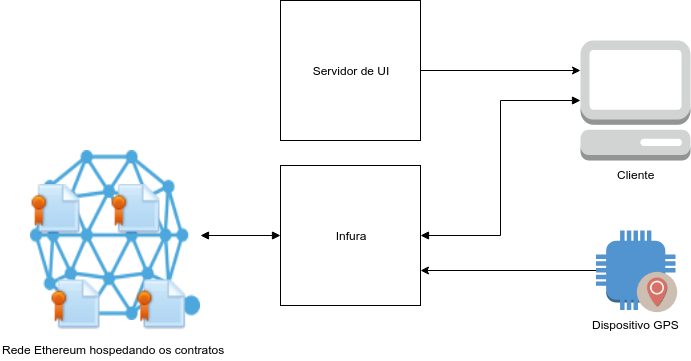
\includegraphics[width=0.7\textwidth]{Cap2/full_ethereum_architecture.png}
\caption{Arquitetura baseada 100\% na rede ethereum.}
\label{full_ethereum_architecture}
\end{figure}

Como pode-se observar na figura \ref{full_ethereum_architecture}, essa arquitetura é composta por 5 componentes:

\begin{itemize}
	\item \textbf{Cliente:} O cliente representa a aplicação web desenvolvida com a framework React (\href{http://www.reactjs.org}{http://www.reactjs.org}) e é responsável por criar um interface gráfica na qual as pessoas possam observar e interagir com os contratos de uma forma amigável.
    \item \textbf{Servidor de UI:} É um servidor de recursos estáticos desenvolvido em Nodejs (\href{http://www.nodejs.org}{http://www.nodejs.org}) com a framework Express (\href{http://www.express.com}{http://www.express.com}). Tal servidor provê o arquivo javascript que contém o código do cliente desenvolvido em React, bem como as imagens da aplicação web.
    \item \textbf{Infura:} Infura (\href{https://infura.io/}{https://infura.io/}) é um serviço web que prove acesso a rede Ethereum por meio de uma API REST. Esse serviço abstrai a complexidade de criar e manter um nó próprio conectado a rede Ethereum.
    \item \textbf{Rede Ethereum:} Representa a rede Ethereum composta por nós espalhados pelo mundo todo.
    \item \textbf{Contratos:} Representa os contratos de seguro automotivo criados e mantidos pelos usuários da aplicação.
    \item \textbf{Dispositivo GPS:} O dispositivo GPS é responsável por enviar constantemente a localização do carro dos participantes do contrato de seguro automotivo para a rede Ethereum. Para manter a privacidade dos usuários, o envio da latitude e longitude é criptografado.
\end{itemize}

Nas seções abaixo, será dado enfoque nos principais componentes do sistema: os contratos, o cliente e o dispositivo GPS.

\subsection{Contratos}

Foram desenvolvidos dois contratos inteligentes, o primeiro deles, SmartCarInsuranceContractFactory, é um contrato responsável por criar e rastrear todos contratos de seguro automotivo. Já o segundo contrato desenvolvido, SmartCarInsuranceContract, representa o próprio contrato de seguro automotivo. O código completo dos contratos está disponível no GitHub (\href{https://github.com/marcoprado17/scife-contracts}{https://github.com/marcoprado17/scife-contracts}).

\begin{figure}[h!]
\centering
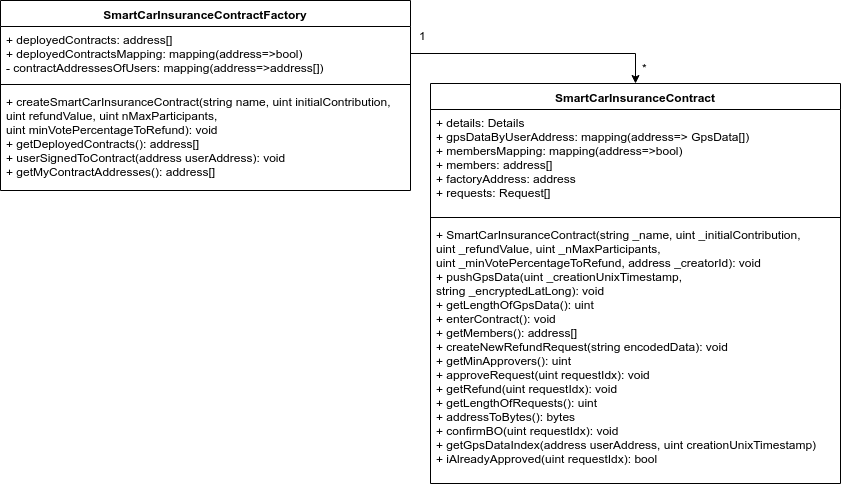
\includegraphics[width=1\textwidth]{Cap2/SmartCarInsuranceContractFactory_and_SmartCarInsuranceContract.png}
\caption{SmartCarInsuranceContractFactory e SmartCarInsuranceContract.}
\label{factory_and_contracts}
\end{figure}

Utilizar um contrato que cria outros contratos é interessante por dois motivos:

\begin{enumerate}
\item Facilita com que os usuários façam o deploy de um novo contrato automotivo no próprio browser. Para tanto, o código do cliente interage com SmartCarInsuranceContractFactory por meio do serviço do Infura para criar um novo contrato;
\item Como todo novo SmartCarInsuranceContract é criado por SmartCarInsuranceContractFactory, o próprio contrato SmartCarInsuranceContractFactory se torna o local ideal para armazenar todos os SmartCarInsuranceContract criados.
\end{enumerate}

Conforme se observa na figura \ref{factory_and_contracts}, um contrato se asemelha muito a uma classe em uma linguagem orientada a objetos: o contrato define um modelo de uma entidade que possui diferentes atributos e métodos. Tal modelo da origem a múltiplas instâncias dessa entidade, sendo que cada instância de contrato criado possui um endereço associado na rede Ethereum.

\subsubsection{SmartCarInsuranceContractFactory}

Segue abaixo o código comentado do contrato SmartCarInsuranceContractFactory:

\begin{code}
\begin{minted}[
frame=lines,
fontsize=\footnotesize,
linenos
]{javascript}
// Utilizando a versão 0.4.17 da linguagem Solidity
pragma solidity ^0.4.17;

contract SmartCarInsuranceContractFactory {
    // Array contendo os endereços ethereum de todos os contratos 
    // SmartCarInsuranceContract que SmartCarInsuranceContractFactory 
    // gerou
    address[] public deployedContracts;
    // Hash table para checagem rápida se certo endereço 
    // ethereum representa um contrato SmartCarInsuranceContract 
    // deployado por SmartCarInsuranceContractFactory
    mapping(address => bool) public deployedContractsMapping;
    // Mapeia os contratos SmartCarInsuranceContract que cada 
    // usuário participa
    mapping(address => address[]) contractAddressesOfUsers;

    // Método que cria uma nova instância de SmartCarInsuranceContract
    function createSmartCarInsuranceContract(
        string name,
        uint initialContribution,
        uint refundValue,
        uint nMaxParticipants,
        uint minVotePercentageToRefund
    ) public {
        // Criando uma nova instância de um contrato 
        // SmartCarInsuranceContract
        address newContractAddress = new SmartCarInsuranceContract(
            name,
            initialContribution,
            refundValue,
            nMaxParticipants,
            minVotePercentageToRefund, 
            msg.sender
        );
        // Armazenando o contrato deployado em deployedContracts
        deployedContracts.push(newContractAddress);
        // Adicionando à hash table deployedContractsMapping o 
        // endereço do novo contrato deployado
        deployedContractsMapping[newContractAddress] = true;
    }

    // Obtenção de deployedContracts
    function getDeployedContracts() public view returns (address[]) {
        return deployedContracts;
    }

    // Adiciona à contractAddressesOfUsers que userAddress agora faz 
    // parte do contrato SmartCarInsuranceContract que chamou essa 
    // função (msg.sender)
    function userSignedToContract(address userAddress) public{
        // Garantindo que quem chamou userSignedToContract seja de 
        // fato um contrato SmartCarInsuranceContract deployado 
        // por SmartCarInsuranceContractFactory
        require(deployedContractsMapping[msg.sender]);
        contractAddressesOfUsers[userAddress].push(msg.sender);
    }

    // Obtendo a array contendo os endereços dos contratos 
    // SmartCarInsuranceContract que o usuário que chamou essa 
    // função participa
    function getMyContractAddresses() public view returns (address[]){
        return contractAddressesOfUsers[msg.sender];
    }
}
\end{minted}
\caption{SmartCarInsuranceContractFactory}
\label{lst:SmartCarInsuranceContractFactory}
\end{code}

\subsubsection{SmartCarInsuranceContract}

Segue abaixo o código comentado de SmartCarInsuranceContract:

\begin{code}
\begin{minted}[
frame=lines,
fontsize=\footnotesize,
linenos
]{javascript}
contract SmartCarInsuranceContract {
    // Definindo a struct Details, tal struct armazena 
    // os principais dados do contrato
    struct Details {
        // Nome do contrato
        string name;
        // Contribuição inicial para participar do contrato
        uint initialContribution;
        // Valor do reembolso em caso de furto e roubo
        uint refundValue;
        // Número máximo de participantes
        uint nMaxParticipants;
        // Percentagem mínima de votos para liberar
        // o reembolso de caso de roubo ou furto
        uint minVotePercentageToRefund;
        // Endereço ethereum do criador desse contrato
        address creatorId;
        // Número de participantes do contrato
        uint nParticipants;
    }

    // Definindo a struct GpsData, tal struct armazena
    // uma amostra dos dados de gps de um usuário do contrato
    struct GpsData {
        // Unix timestamp do bloco ethereum que recebeu 
        // tal GpsData
        uint blockUnixTimestamp;
        // Tempo em que tal amostra foi colhida, esse valor
        // é enviado pelo usuário
        uint creationUnixTimestamp;
        // String encriptada contendo a latitude e longitude 
        // dessa amostra de sinal gps
        string encryptedLatLong;
    }

    // Definindo a struct Request, tal struct representa
    // uma requisição de reembolso criado por um usuário
    // do contrato
    struct Request {
        // String base64 encoded contendo um json com as informações
        // necessárias para a requisição:
        // {
        //     unixTimesptampOfTheft: 1232143213,
        //     latTheft: 1.2231
        //     longTheft: 2.2314
        //     keysOfGpsData = [
        //         [122348763244, "secret"], # [unixTimestamp, key]
        //         [122348763244, "secret"],
        //         ...
        //     ]
        // }
        string encodedData;
        // Endereço ethereum de quem criou a requisição de reembolso
        address creatorAddress;
        // Hash table que mapeia o endereço ethereum de quem aprovou
        // tal requisição de reembolso
        mapping(address => bool) approvers;
        // Número de usuários que aprovaram tal requisição de 
        // reembolso
        uint nApprovers;
        // Bool que indica se tal requisição de reembolso foi
        // aprovada pela polícia
        bool boConfirmed;
        // Unix timestamp do bloco ethereum que recebeu essa
        // nova requisição de reembolso
        uint unixTimestampOfBlock;
        // Bool que indica se o reembolso já foi efetuado ou não
        bool refundMade;
    }

    // Detalhes desse contrato de seguro automotivo
    Details public details;
    // Hash table que armazena os dados de gps de cada
    // membro do contrato
    mapping(address => GpsData[]) public gpsDataByUserAddress;
    // Hash table que armazena o endereço ethereum dos membros
    // do contrato
    mapping(address => bool) public membersMapping;
    // Array com o endereço ethereum de todos os membros do contrato
    address[] public members;
    // Endereço ethereum do contrato SmartCarInsuranceContractFactory
    // que deu origem a este contrato
    address public factoryAddress;
    // Array contento todas as requisições de reembolso feitas
    // nesse contrato
    Request[] public requests;
    
    // Contrutor de SmartCarInsuranceContract. Serve para criar
    // uma nova instância deste contrato
    function SmartCarInsuranceContract(
        string _name,
        uint _initialContribution,
        uint _refundValue,
        uint _nMaxParticipants,
        uint _minVotePercentageToRefund,
        address _creatorId
    ) public {
        // Garantindo alguns requisitos básicos para criação do contrato
        require(_initialContribution > 0);
        require(_refundValue > 0);
        require(_nMaxParticipants > 0);
        require(_minVotePercentageToRefund >= 0 && 
        _minVotePercentageToRefund <= 100);
        // Criando os detalhes desse contrato
        details = Details({
            name: _name,
            initialContribution: _initialContribution,
            refundValue: _refundValue,
            nMaxParticipants: _nMaxParticipants,
            minVotePercentageToRefund: _minVotePercentageToRefund,
            creatorId: _creatorId,
            nParticipants: 0
        });
        // Atualizando o endereço de quem criou a instância desse contrato
        factoryAddress = msg.sender;
    }

    // Método que adiciona um novo GpsData de um membro do contrato
    function pushGpsData(
        uint _creationUnixTimestamp, 
        string _encryptedLatLong) public {
        // Garantindo que quem chamou esse método seja um membro do contrato
        require(membersMapping[msg.sender]);
        uint l = gpsDataByUserAddress[msg.sender].length;
        if(l > 0){
            // Garantindo que unix timestamp fornecido pelo gps
            // seja maior do que o timestamp da última amostra
            // de sinal gps
            require(_creationUnixTimestamp > 
                gpsDataByUserAddress[msg.sender][l-1].creationUnixTimestamp);
        }
        // Criando uma nova instância de GpsData
        GpsData memory newGpsData = GpsData({
            blockUnixTimestamp: block.timestamp,
            creationUnixTimestamp: _creationUnixTimestamp,
            encryptedLatLong: _encryptedLatLong
        });

        // Adicionando a nova instância de GpsData criada para
        // a hash table gpsDataByUserAddress
        gpsDataByUserAddress[msg.sender].push(newGpsData);
    }

    // Método para a obtenção do comprimento da array que armazena
    // os dados de gps de um usuário específico
    function getLengthOfGpsData(address _address) 
    public view returns(uint) {
        return gpsDataByUserAddress[_address].length;
    }

    // Método que um possível membro do contrato chama para participar
    // do contrato de seuro automotivo em questão
    function enterContract() public payable{
        // Garantindo que o possível membro envie, ao chamar essa
        // função, um valor igual a contribuição inicial estabelecida
        // no momento em que esse contrato foi gerado
        require(msg.value == details.initialContribution);
        // Garantindo que quem chamou essa função não seja
        // membro do contrato ainda
        require(!membersMapping[msg.sender]);
        // Garantindo que o contrato em questão ainda não excederá
        // o número máximo de participantes
        require(members.length < details.nMaxParticipants);
        // Incrmentando o número de participantes
        details.nParticipants++;
        // Adicionando o novo membro à membersMapping e members
        membersMapping[msg.sender] = true;
        members.push(msg.sender);
        // Informando a SmartCarInsuranceContractFactory que msg.sender
        // agora é um membro deste contrato
        SmartCarInsuranceContractFactory smartCarInsuranceContractFactory = 
            SmartCarInsuranceContractFactory(factoryAddress);
        smartCarInsuranceContractFactory.userSignedToContract(msg.sender);
    }

    // Obtendo a array com os endereços ethereum dos membros deste contrato
    function getMembers() public view returns (address[]) {
        return members;
    }

    // Método chamado para a criação de uma nova requisição de reembolso
    /*
        encodedData representa a base64 encode do objeto abaixo:
        {
            unixTimesptampOfTheft: 1232143213,
            latTheft: 1.2231
            longTheft: 2.2314
            keysOfGpsData = [
                [122348763244, "secret"], # [unixTimestamp, key]
                [122348763244, "secret"],
                ...
            ]
        }
     */
    function createNewRefundRequest(string encodedData) public {
        // Garantindo que quem chamou esse método (msg.sender)
        // seja um membro do contrato
        require(membersMapping[msg.sender]);
        // Criando uma nova instância da struct Request com
        // os devidos dados
        Request memory newRequest;
        newRequest.encodedData = encodedData;
        newRequest.creatorAddress = msg.sender;
        newRequest.boConfirmed = false;
        newRequest.nApprovers = 0;
        newRequest.unixTimestampOfBlock = block.timestamp;
        newRequest.refundMade = false;
        // Adicionando a instância de request criada à
        // array requests
        requests.push(newRequest);
    }

    // Obtendo o número mínimo de membros que devem aprovar
    // uma requisição de reembolso para ela ser liberada
    function getMinApprovers() public view returns (uint) {
        // Retornando 0 caso details.minVotePercentageToRefund == 0
        if(details.minVotePercentageToRefund == 0) {
            return 0;
        }
        // Retornando ceil de
        // details.minVotePercentageToRefund*details.nParticipants/100
        // caso contrário
        uint multi = details.minVotePercentageToRefund * details.nParticipants;
        bool hasRemainder = true;
        if(multi % 100 == 0){
            hasRemainder = false;
        }
        uint minApprovers = multi / 100;
        if(hasRemainder){
            minApprovers++;
        }
        return minApprovers;
    }

    // Método que um usuário chama para aprovar determinada
    // requisição de reembolso
    function approveRequest(uint requestIdx) public{
        // Garantindo que msg.sender seja um membro do contrato
        require(membersMapping[msg.sender]);
        // Garantindo que msg.sender não tenha aprovado tal
        // requisão antes
        require(!requests[requestIdx].approvers[msg.sender]);
        // Adicionando aos aprovadores da requisição o endereço
        // de msg.sender
        requests[requestIdx].approvers[msg.sender] = true;
        // Aumentando o número de pessoas que aprovaram
        // tal requisição
        requests[requestIdx].nApprovers++;
        // Efetuando o reembolso caso os três requisitos abaxo
        // sejam atendidos
        // a) O número de membros aprovadores do reembolso seja 
        // maior ou igual ao mínimo requerido;
        // b) O contrato possua uma quantia de ethereum maior ou igual
        // ao valor do reembolso;
        // c) O boletim de ocorrência de furto ou roubo já tenha
        // sido confirmado pela polícia.
        uint minApprovers = getMinApprovers();
        if(
            requests[requestIdx].nApprovers >= minApprovers
            && address(this).balance >= details.refundValue
            && requests[requestIdx].boConfirmed
        ){
            requests[requestIdx].creatorAddress.send(details.refundValue);
            requests[requestIdx].refundMade = true;
        }
    }

    // Liberando o reembolso caso todos os requisitos
    // para liberação do reembolso estejam etendidos
    function getRefund(uint requestIdx) public {
        require(requests[requestIdx].creatorAddress == msg.sender);
        require(requests[requestIdx].boConfirmed);
        uint minApprovers = getMinApprovers();
        require(requests[requestIdx].nApprovers >= minApprovers);
        require(address(this).balance >= details.refundValue);
        requests[requestIdx].creatorAddress.transfer(details.refundValue);
        requests[requestIdx].refundMade = true;
    }

    // Obtendo o comprimento da array requests
    function getLengthOfRequests() public view returns(uint) {
        return requests.length;
    }

    // Função que converte um address para bytes
    function addressToBytes(address _addr) public pure returns(bytes) {
        bytes32 value = bytes32(uint256(_addr));
        bytes memory alphabet = "0123456789abcdef";

        bytes memory str = new bytes(51);
        str[0] = "0";
        str[1] = "x";
        for (uint i = 0; i < 20; i++) {
            str[2+i*2] = alphabet[uint(value[i + 12] >> 4)];
            str[3+i*2] = alphabet[uint(value[i + 12] & 0x0f)];
        }
        return str;
    }

    // Função que confirma se o BO de furto ou roubo
    // de uma determinada requisição de reembolso foi feito
    // com sucesso
    function confirmBO(uint requestIdx) public {
        // Garantindo que o BO ainda não tenha sido confirmado
        require(!requests[requestIdx].boConfirmed);
        // Garantindo que msg.sender == 
        // "0x5e924ac15745b75e0d23afd68d1bb1adb8f43689"
        bytes memory validBoSenderAddress = 
        "0x5e924ac15745b75e0d23afd68d1bb1adb8f43689";
        bytes memory senderAddress = addressToBytes(msg.sender);
        bool validSender = true;
        for(uint i = 0; i < validBoSenderAddress.length; i++){
            if(validBoSenderAddress[i] != senderAddress[i]){
                validSender = false;
            }
        }
        require(validSender);
        // Confirmando o BO
        requests[requestIdx].boConfirmed = true;
    }

    // Obtendo o indice do GpsData na array 
    // gpsDataByUserAddress[userAddress] que foi criado
    // o mais proximo possível de creationUnixTimestamp
    function getGpsDataIndex(
        address userAddress, 
        uint creationUnixTimestamp) public view returns(uint){
        if(gpsDataByUserAddress[userAddress].length == 0){
            return 0;
        }
        if(creationUnixTimestamp <= 
        gpsDataByUserAddress[userAddress][0].creationUnixTimestamp){
            return 0;
        }
        if(
            creationUnixTimestamp >= 
            gpsDataByUserAddress[userAddress]
            [gpsDataByUserAddress[userAddress].length-1]
            .creationUnixTimestamp){
            return gpsDataByUserAddress[userAddress].length-1;
        }
        // Efetuando uma busca binária para obtenção do indice
        // de GpsData com creationUnixTimestamp mais próximo
        // do desejado
        uint low = 0;
        uint high = gpsDataByUserAddress[userAddress].length-1;
        while (low <= high) {
            uint mid = (low + high) / 2;
            if(gpsDataByUserAddress[userAddress]
            [mid].creationUnixTimestamp > 
            creationUnixTimestamp){
                high = mid - 1;
            }
            else if (gpsDataByUserAddress[userAddress][mid]
            .creationUnixTimestamp < creationUnixTimestamp){
                low = mid + 1;
            }
            else {
                return mid;
            }
        }
        return low;
    }

    // Método que retorna um bool indicando se msg.sender
    // já aprovou ou não o a requisição de índice requestIdx
    function iAlreadyApproved(uint requestIdx) public view returns (bool) {
        require(membersMapping[msg.sender]);
        return requests[requestIdx].approvers[msg.sender];
    }
}
\end{minted}
\caption{SmartCarInsuranceContract}
\label{lst:SmartCarInsuranceContract}
\end{code}

\subsection{Cliente}

O código do cliente foi desenvolvido com a framework React e encontra-se disponível no GitHub (\href{https://github.com/marcoprado17/scife-ui-service}{https://github.com/marcoprado17/scife-ui-service}). Tal aplicação web contém contém 5 páginas.

\subsubsection{Páginas da aplicação}

\begin{itemize}
\item \textbf{Home Page:} Página principal da aplicação, contém uma explicação básica de como a aplicação e contrato funciona. Um screenshot dessa página pode ser encontrado na figura \ref{home_page}.
\item \textbf{Criação de um novo contrato:} Página que contém um formulário com os dados necessários para a criação de um novo contrato. Um screenshot dessa página pode ser encontrado na figura \ref{new_contract}.
\item \textbf{Participação em um contrato existente:} Página que exibe todos os contratos criados com um botão para o usuário participar do contrato. Um screenshot dessa página pode ser encontrado na figura \ref{participate_existent_contract}.
\item \textbf{Administrar meu contratos:} Página que exibe informações sobre os contratos que o usuário participa. Para cada contrato há 4 abas:
	\begin{itemize}
	\item \textbf{Detalhes:} Informação completa sobre tal contrato. Um screenshot dessa aba pode ser visto na figura \ref{my_contracts_details}
    \item \textbf{Participantes:} Lista o endereço dos participantes do contrato. Um screenshot dessa aba pode ser visto na figura \ref{my_contracts_participants}
    \item \textbf{Requisições:} Lista com as requisições de reembolso feitas por membros do contrato. Nessa aba, o usuário pode aprovar ou não a requisição em questão. Um screenshot dessa aba pode ser visto na figura \ref{my_contracts_requests}
    \item \textbf{Nova Requsição:} Essa aba contém um formulário para que o usuário crie uma nova requisição de reembolso. Um screenshot dessa aba pode ser visto na figura \ref{my_contracts_new_request}
	\end{itemize}
\item \textbf{Confirmação de BO:} Página na qual são exibidos as requisições de reembolso e na qual, apenas a conta Ethereum administrada pela polícia pode aprovar se um boletim de ocorrência condizente com a requisição em questão foi registrado. Um screenshot dessa página pode ser encontrado na figura \ref{confirm_bo}.
\end{itemize}

\begin{figure}[h!]
\centering
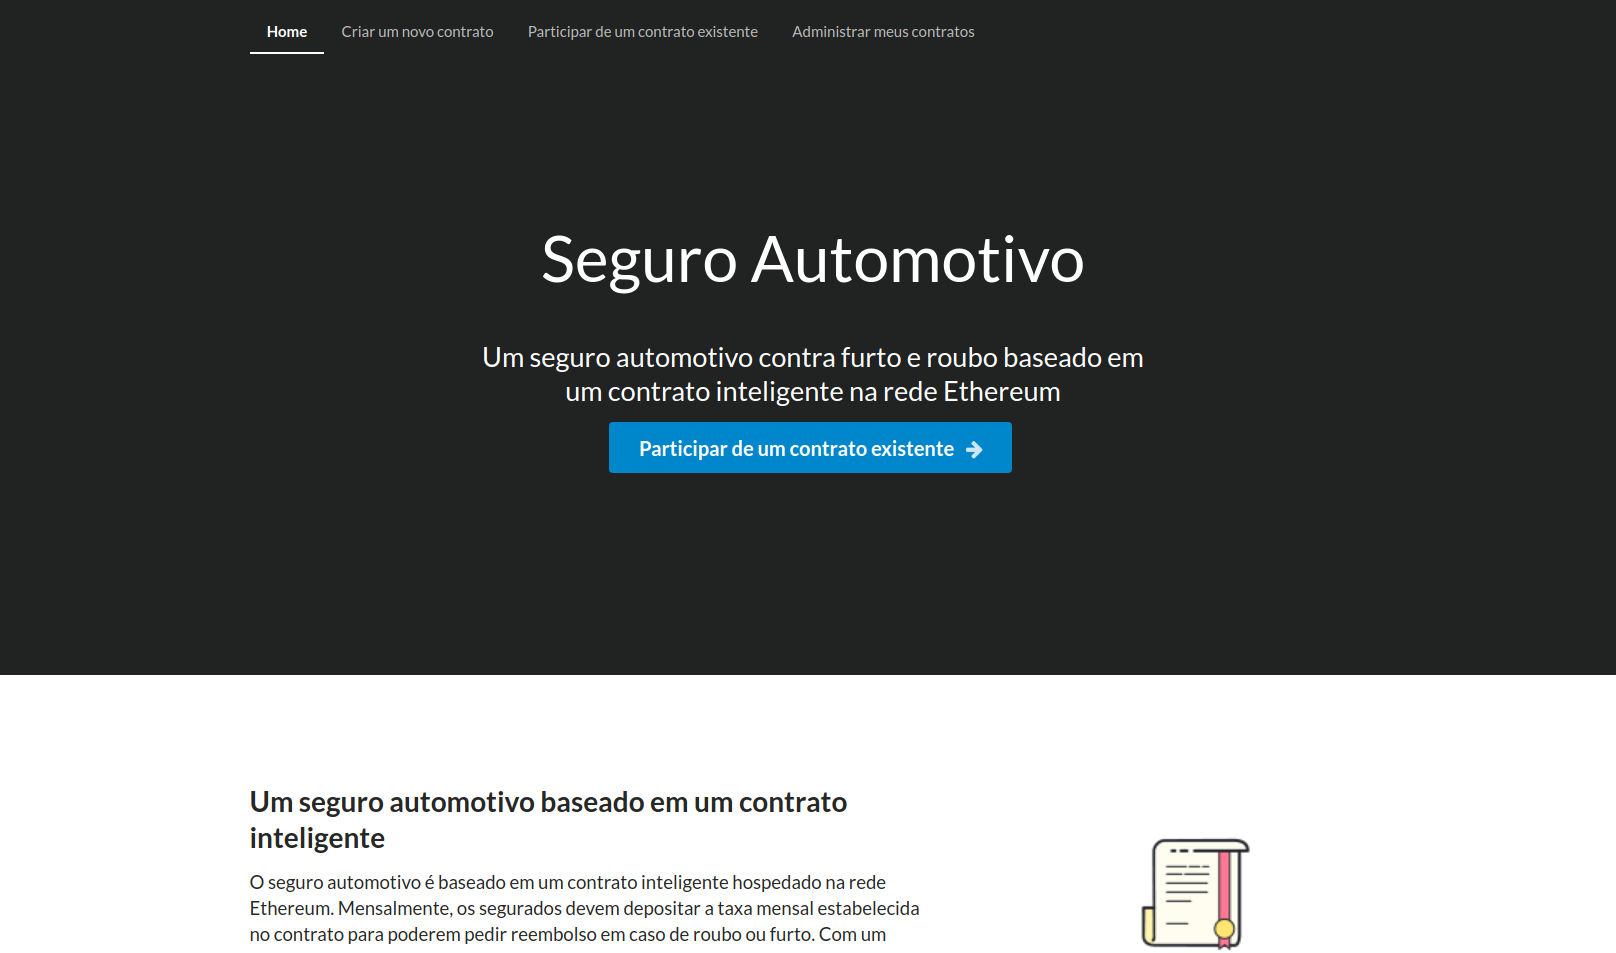
\includegraphics[width=0.9\textwidth]{Cap2/home_page.png}
\caption{Home page da aplicação.}
\label{home_page}
\end{figure}

\begin{figure}[h!]
\centering
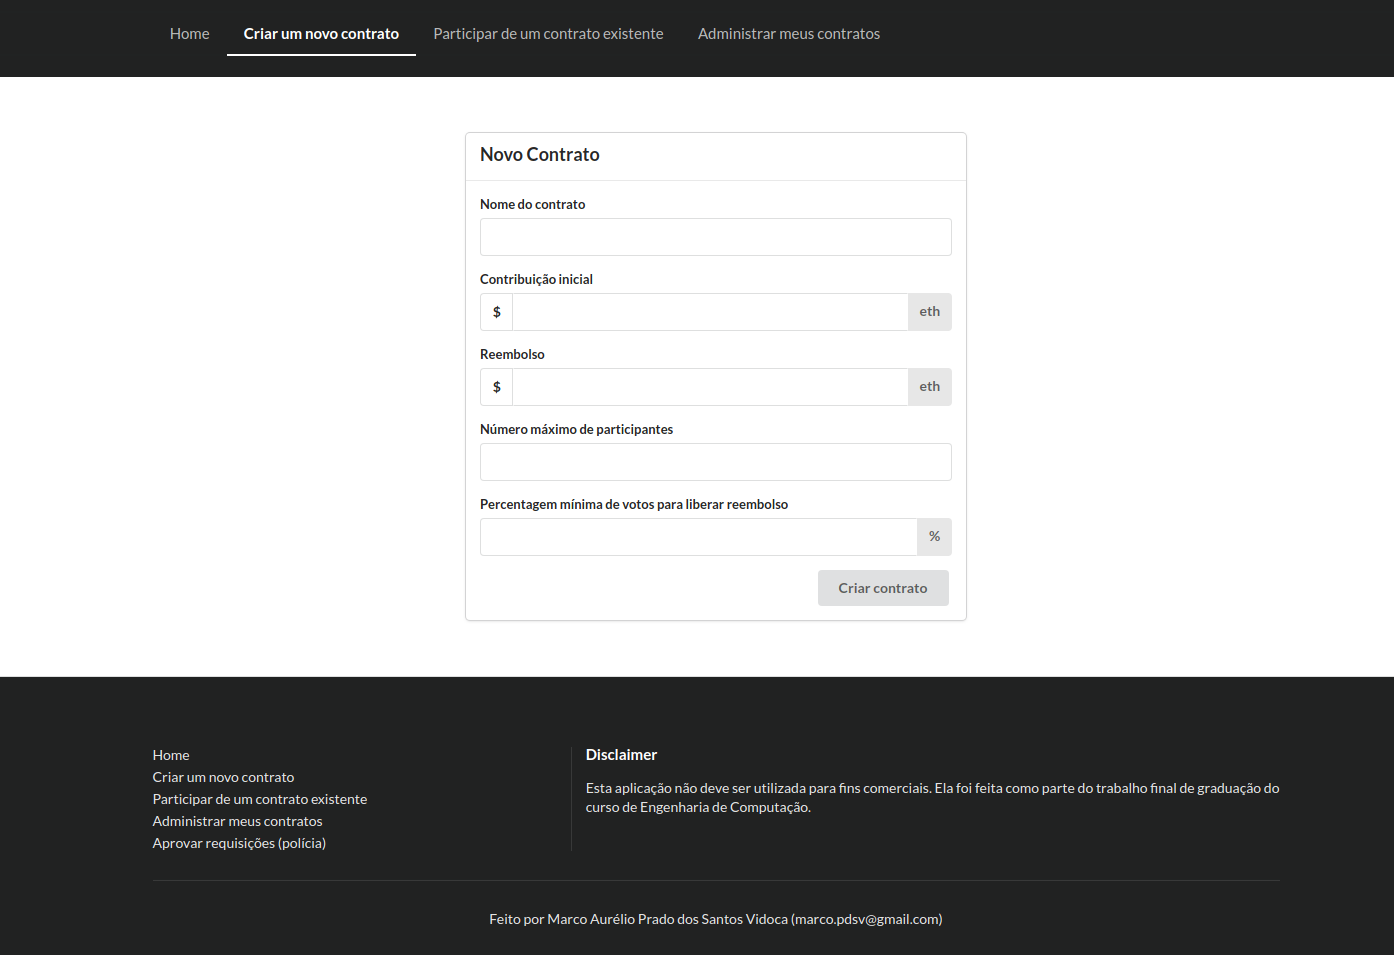
\includegraphics[width=0.9\textwidth]{Cap2/new_contract.png}
\caption{Formulário para a criação de um novo contrato de seguro automotivo.}
\label{new_contract}
\end{figure}

\begin{figure}[h!]
\centering
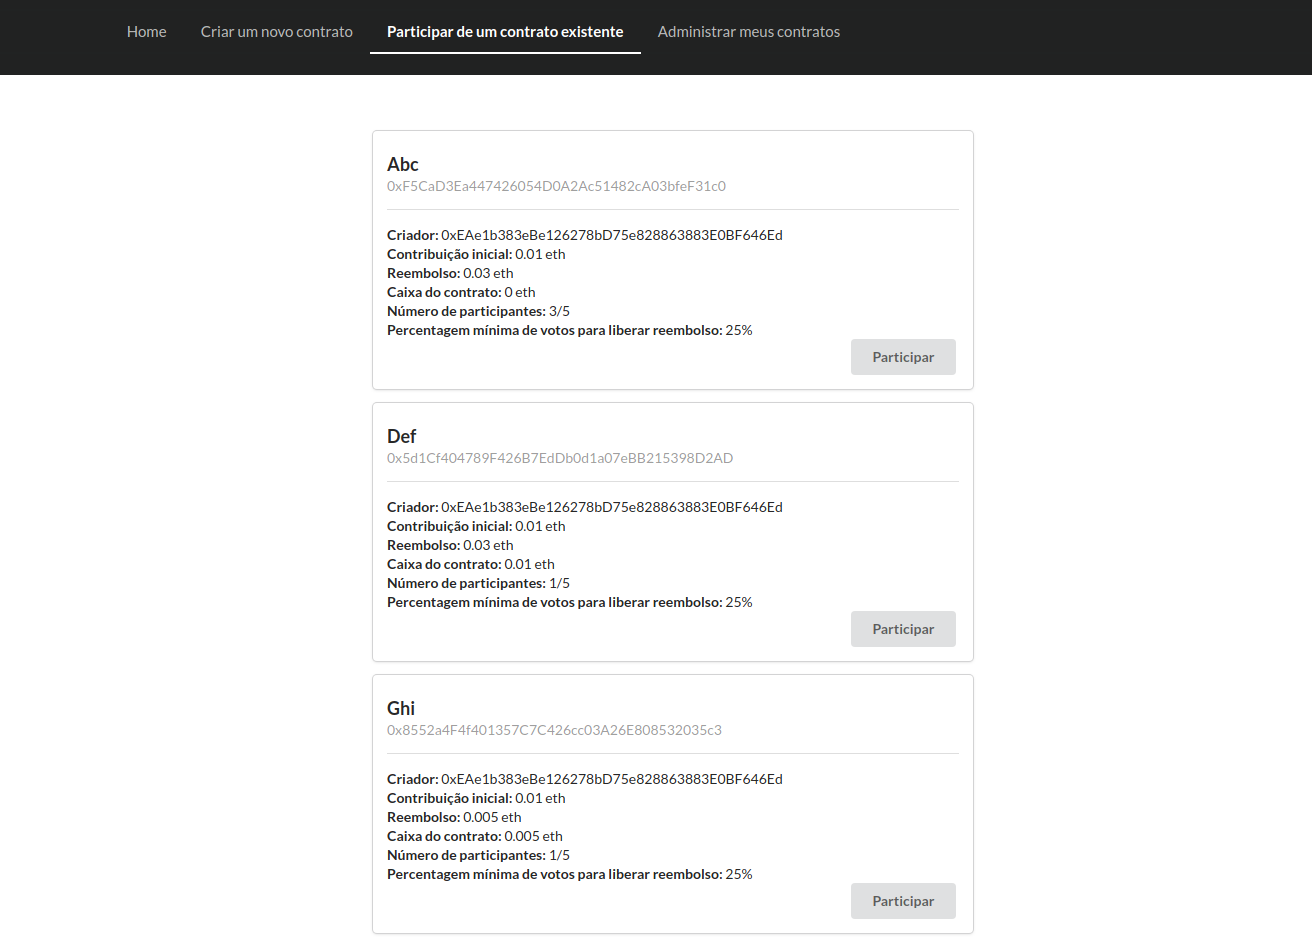
\includegraphics[width=0.9\textwidth]{Cap2/participate_existent_contract.png}
\caption{Lista com os contratos criados e os quais qualquer pessoa pode participar mediante ao pagamento de taxa.}
\label{participate_existent_contract}
\end{figure}

\begin{figure}[h!]
\centering
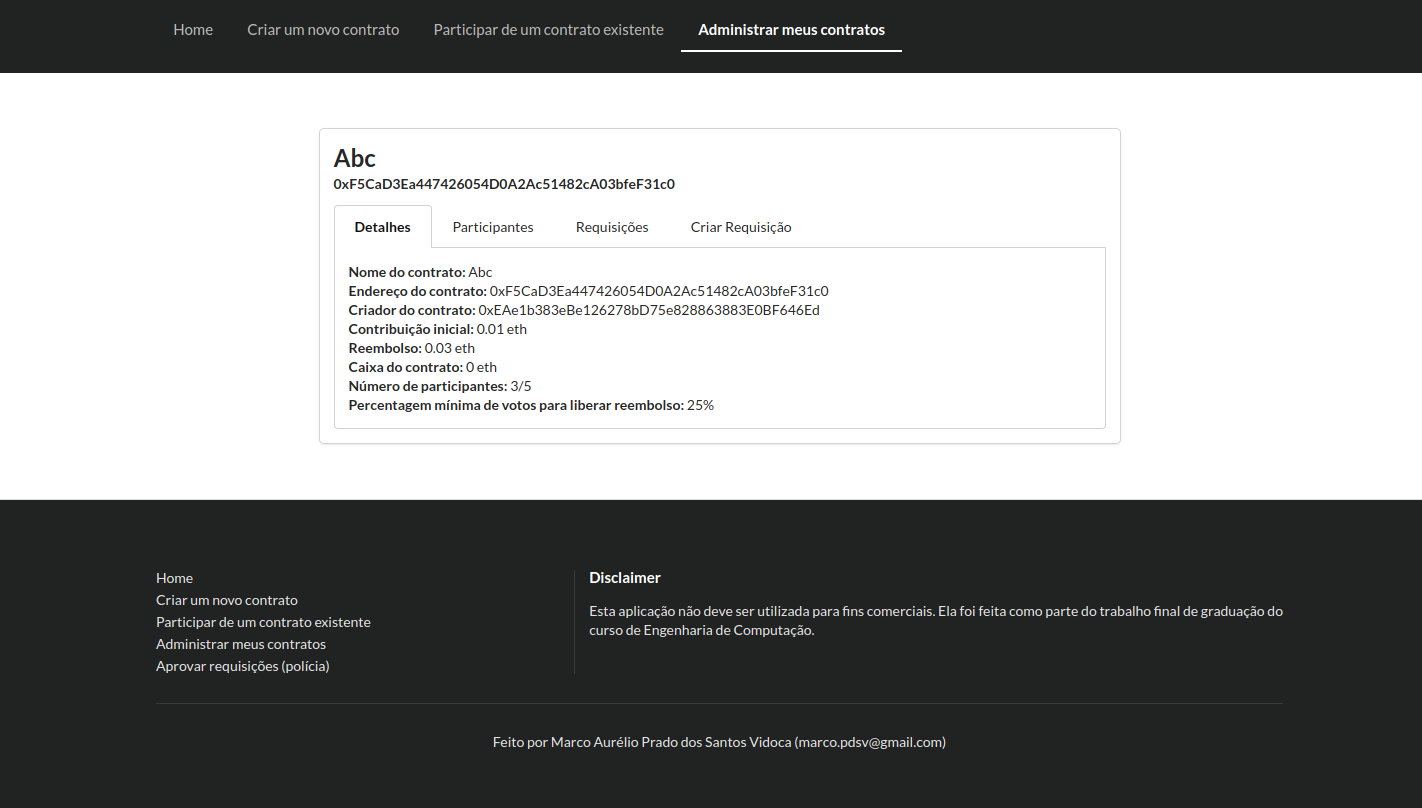
\includegraphics[width=0.9\textwidth]{Cap2/my_contracts_details.png}
\caption{Página contendo os contratos ativos da pessoa que está acessando a aplicação. Nesse caso, se vê a aba de detalhes do contrato.}
\label{my_contracts_details}
\end{figure}

\begin{figure}[h!]
\centering
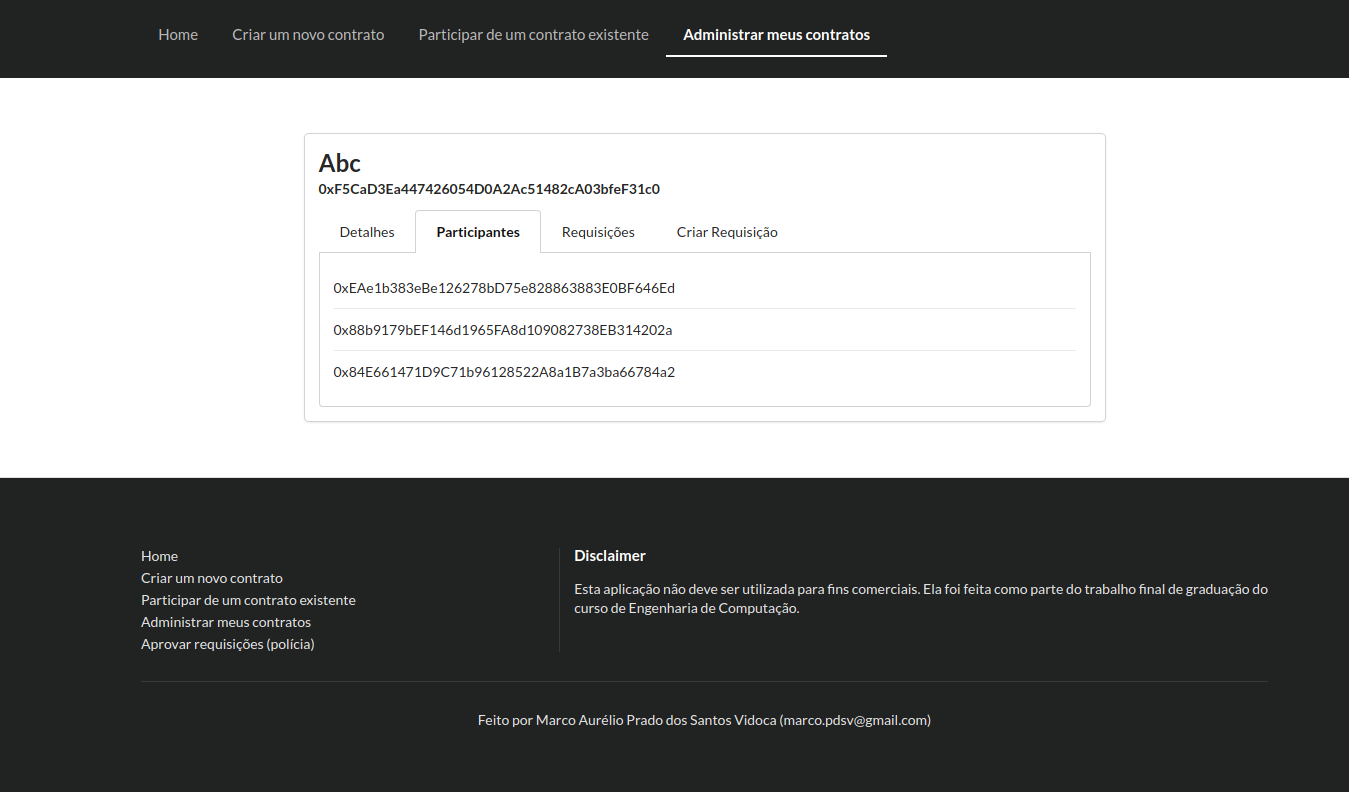
\includegraphics[width=0.9\textwidth]{Cap2/my_contracts_participants.png}
\caption{Página contendo os contratos ativos da pessoa que está acessando a aplicação. Nesse caso, se vê a aba que exibe o endereço da conta Ethereum de quem participa do contrato.}
\label{my_contracts_participants}
\end{figure}

\begin{figure}[h!]
\centering
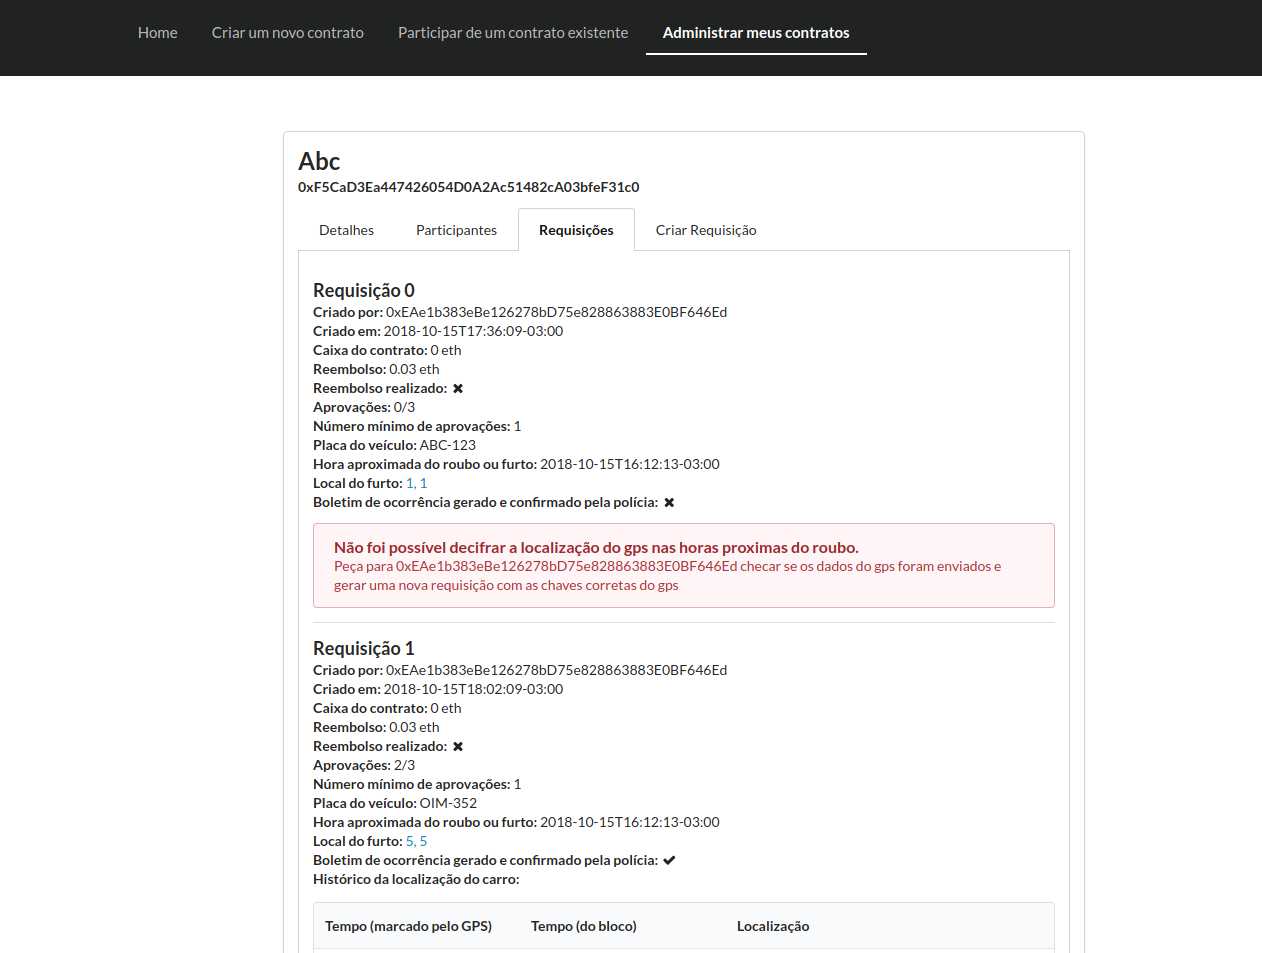
\includegraphics[width=0.9\textwidth]{Cap2/my_contracts_requests.png}
\caption{Página contendo os contratos ativos da pessoa que está acessando a aplicação. Nesse caso, se vê a aba que exibe as requisições de reembolso feitas pelos participantes do contrato.}
\label{my_contracts_requests}
\end{figure}

\begin{figure}[h!]
\centering
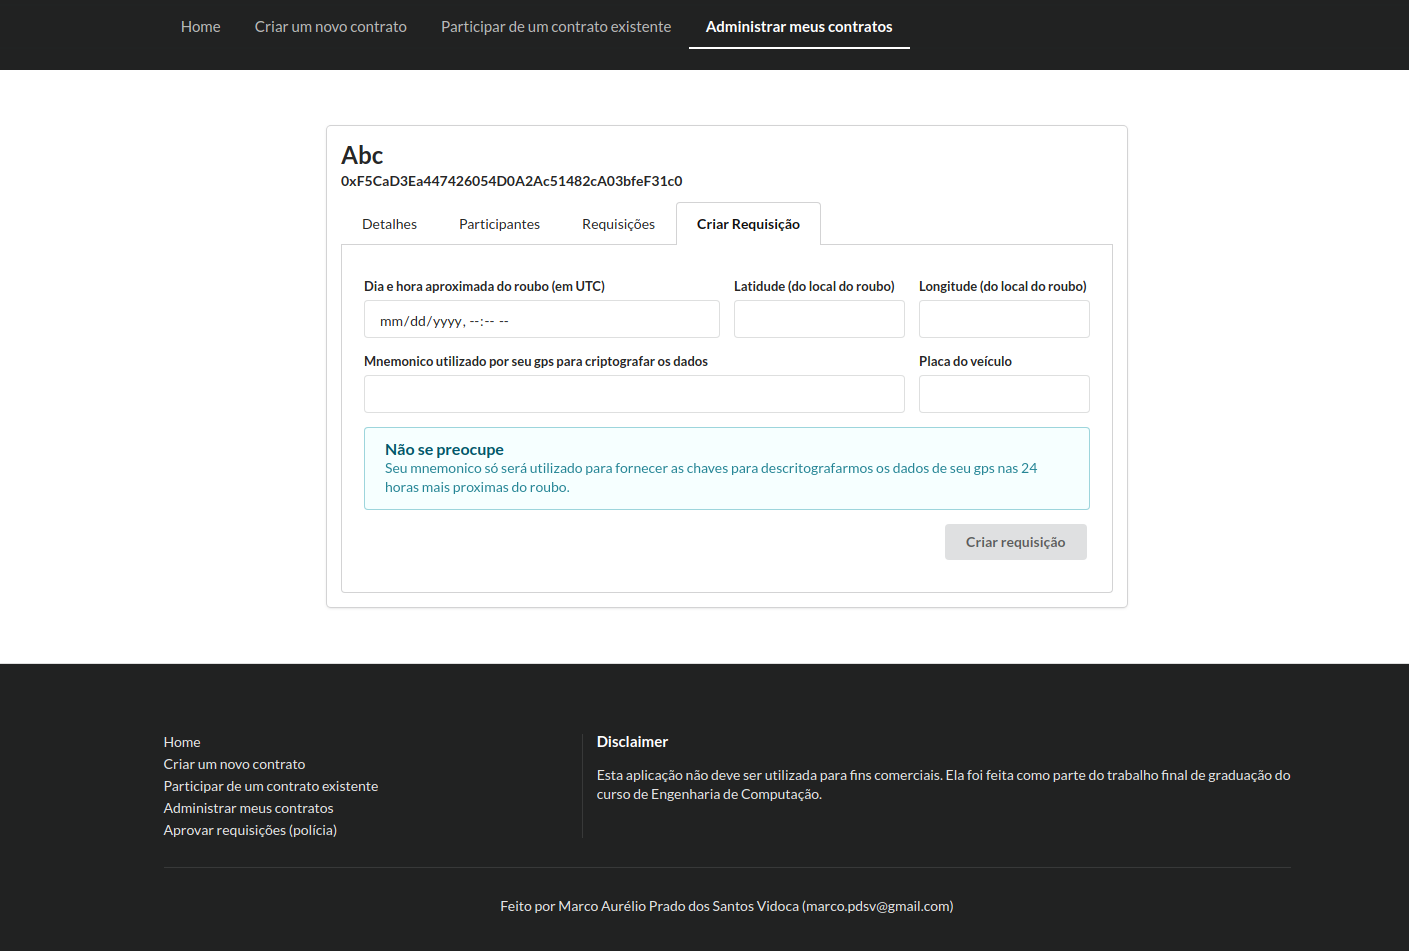
\includegraphics[width=0.9\textwidth]{Cap2/my_contracts_new_request.png}
\caption{Página contendo os contratos ativos da pessoa que está acessando a aplicação. Nesse caso, se vê a aba na qual o participante do contrato pode criar uma nova requisição de reembolso.}
\label{my_contracts_new_request}
\end{figure}

\begin{figure}[h!]
\centering
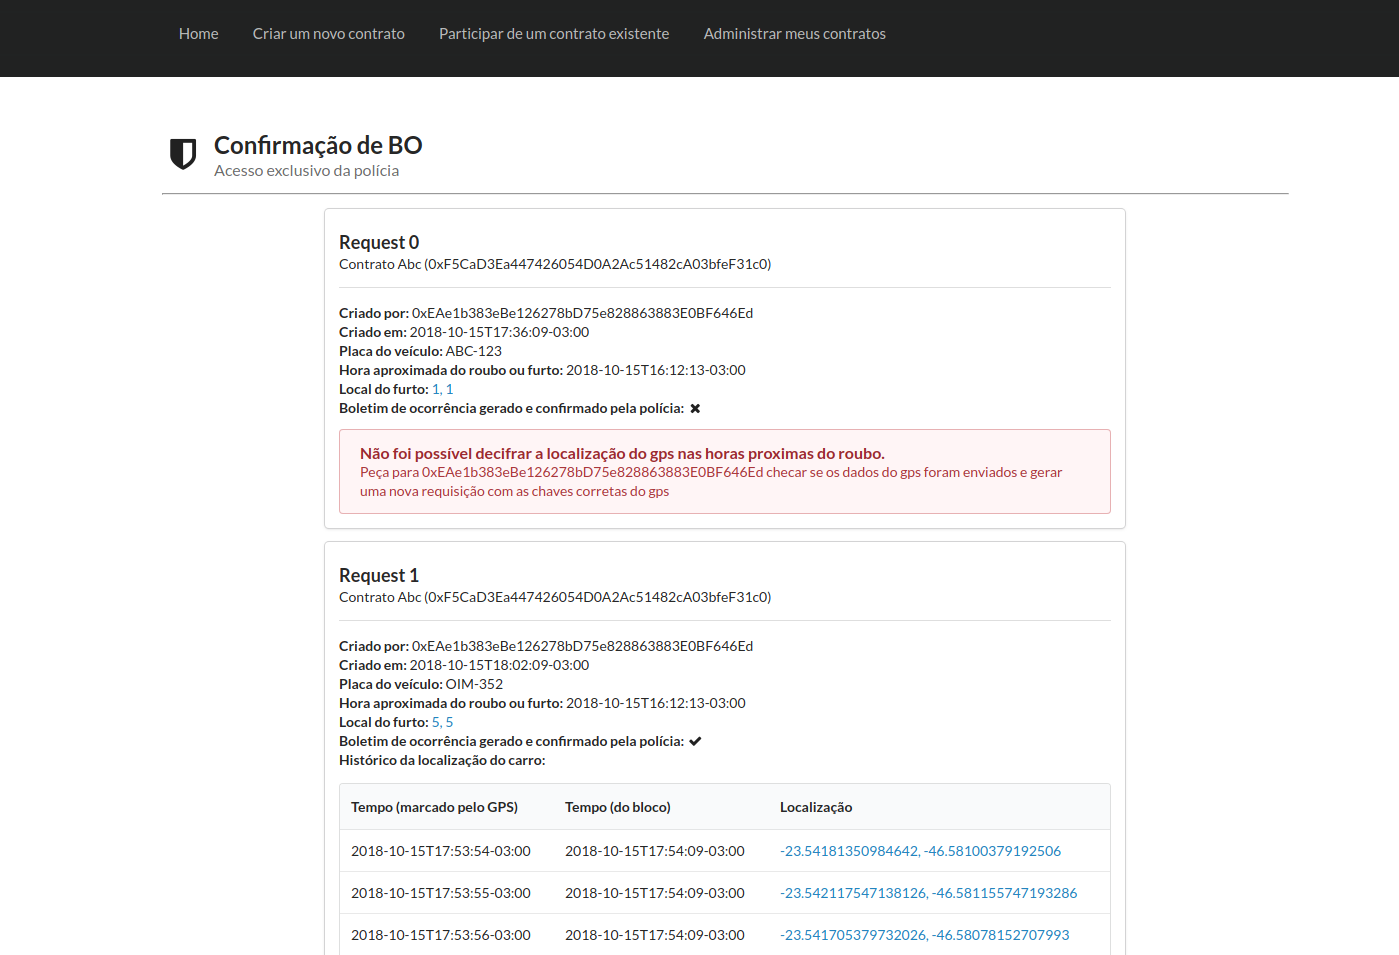
\includegraphics[width=0.9\textwidth]{Cap2/confirm_bo.png}
\caption{Página na qual são exibidos as requisições de reembolso e na qual, apenas a conta Ethereum administrada pela polícia pode aprovar se um boletim de ocorrência condizente com a requisição em questão foi registrado.}
\label{confirm_bo}
\end{figure}

\clearpage
\subsubsection{Comunicação com a Rede Ethereum por meio da lib web3js}

Para a aplicação cliente se comunicar com a rede Ethereum, é utilizada a bliblioteca javascript web3js versão 1.0.0-beta36. Essa biblioteca permite a interação com um nó remoto ou local da rede Ethereum. No código abaixo, pode-se ver como a biblioteca é utilizada na criação de um novo contrato de seguro automotivo:

\begin{code}
\begin{minted}[
frame=lines,
fontsize=\footnotesize,
linenos
]{javascript}
// Importando a lib web3js
import Web3 from 'web3'; 
// Importando o json com as especificações de SmartCarInsuranceContractFactory
import SmartCarInsuranceContractFactory from 
'./build/SmartCarInsuranceContractFactory.json';

// Criando a instância da lib web3 a partir do provedor  do MetaMask
const web3 = new Web3(window.web3.currentProvider);
// Criando uma instância da fábrica de contratos
const smartCarInsuranceContractFactory = new web3.eth.Contract(
    JSON.parse(SmartCarInsuranceContractFactory.interface),
    "0xB7CbfB9d3a64983623f06C410489eA0bCb628B06"
);
// Obtendo as contas cadastradas no MetaMask
const accounts = await web3.eth.getAccounts();

// Chamando o método que cria um novo contrato automotivo, passando
// os parâmetros necessários: nome do contrato, contribuição inicial,
// valor do reembolso, número máximo de participantes e mínima
// percentagem de votos para liberar reembolso
await smartCarInsuranceContractFactory.methods
	.createSmartCarInsuranceContract(
		this.state.contractName,
      	web3.utils.toWei(this.state.initialContribution),
      	web3.utils.toWei(this.state.refundValue),
      	this.state.nMaxParticipants,
      	this.state.minVotePercentageToRefund)
  	.send({
  		from: accounts[0]
	});
\end{minted}
\caption{Biblioteca web3js}
\label{lst:lib_web3js}
\end{code}

Conforme se observa no código acima, o construtor de Web3 recebe window.web3.currentProvider. Para se criar uma instância de um objeto Web3, deve-se passar para o construtor de Web3 um objeto que implemente a interface Provider. Tal objeto é responsável por estabelecer como a lib Web3 irá interagir com o blockchain.

\begin{figure}[h]
\centering
\includegraphics[width=0.7\textwidth]{Cap2/providers.png}
\caption{Strategy pattern com os Providers do Web3.}
\label{providers}
\end{figure}

Na aplicação construída, utilizou-se 3 Providers diferentes:

\begin{itemize}
\item \textbf{MetaMaskProvider:} Metamask é uma extensão do chrome que gerencia as contas dos usuários na rede Ethereum. Ele injeta em toda página web que o usuário visita um Provider com as contas cadastradas pelo usuário e que se comunica com a rede Ethereum utilizando o Infura.
\item \textbf{HDWalletProvider:} Esse provider é utilizado para fazer o deploy de SmartCarInsuranceContractFactory e também na aplicação que simula o gps e envia os dados para o contrato de seuguro automotivo. Esse provider recebe as credenciais da conta Ethereum e a url de accesso do Infura.
\item \textbf{GanacheProvider:} Esse provider é utilizado nos testes dos contratos. O Ganache cria uma rede blockchain Ethereum na máquina local e disponibiliza um provider para se comunicar com rede criada. O Ganache configura tal rede de forma que as transações ocorram rapidamente, criando uma ambiente ideal para testar os contratos antes de fazer o deploy para a rede Ethereum principal.
\end{itemize}

\subsection{Dispositivo GPS}

O dispositivo GPS foi simulado por um código desenvolvido em NodeJs e se encontra disponível no GitHub (\href{https://github.com/marcoprado17/scife-gps-simulator}{https://github.com/marcoprado17/scife-gps-simulator}). O código do simulador foi dividido em dois scripts, o primeiro deles, run.js, é responsável por criar n processos que executam o segundo script, run\_for\_user.js. Esse segundo script, representa o dispositivo GPS de um usuário do sistema e fica constantemente gerando uma latitude e longitude aleatórios a partir de um ponto inicial (figura \ref{gps_location_generator}) para enviar para o contrato após criptografá-los. Seguem abaixo o pseudo código explicando o funcionamento do simulador do dispositivo GPS de um usuário, bem como o código comentado dos principais arquivos:

\begin{enumerate}
\item Obtenção da chave mestre do dispositivo GPS a partir do mnêmonico utilizando o BIP39;
\item Geração inicial da posição do carro, obtendo a latitude a partir de uma distribuição aleatória uniforme entre -23.603244 e -23.504324 e uma longitude a partir de uma distribuição aleatória uniforme entre -46.679381 e -46.561788;
\item Geração de \(\Delta_{lat}\) e \(\Delta_{long}\) a partir de uma distribuição aleatória uniforme entre -0.005 e 0.005;
\item Obtenção das latitudes e longitudes da iteração atual, \(curr_{lat} = curr+{lat} + \Delta_{lat}\) e \(curr_{long} = curr_{long} + \Delta_{long}\);
\item Obtenção Unix Timestamp atual em segundos, \(t_{0}\);
\item Obtenção do índice da chave privada filha a partir da chave privada mestre, \(i = t_{0} - 946684800\). 946684800 representa o Unix Timestamp de 01/01/2000 00:00:00Z. Como a chave mestra pode dar origem a \(2^{32}\) chaves filhas, podemos gerar as chaves privadas que encriptam o dado do sinal GPS até o Unix Timestamp \(t_{1} = 946684800 + 2^{32} = 5241652096\), ou seja, até 02/07/2136 06:28:00Z;
\item Obtenção da chave privada \(k_{priv}\) = i-essima chave filha da chave privada mestre;
\item Encriptação da latitude e longitude do sinal GPS utilizando \(k_{priv}\) e AES256 \cite{aes}.
\item Envio do sinal GPS para o contrato na rede Ethereum;
\item Medição dos dados pertinentes ao envio dessa amostra de sinal GPS para posterior análise.
\end{enumerate}

\begin{figure}[h!]
\centering
\includegraphics[width=0.9\textwidth]{Cap2/gps_location_generator}
\caption{Posição inicial do sinal GPS do carro de um usuário.}
\label{gps_location_generator}
\end{figure}

\clearpage
\begin{code}
\begin{minted}[
frame=lines,
fontsize=\footnotesize,
linenos
]{javascript}
const spawn = require('child_process').spawn;
// Obtendo o arquivo de configurações
const configs = require('./configs');

[...Array(configs.nUsers).keys()].map(user_idx => {
    // Iniciando um processo que executa o script run_for_user.js
    let command = spawn("node", ["run_for_user.js", user_idx]);
    
    // Imprimindo o stout dos processos filhos no processo mãe
    command.stdout.on('data', function (data) {
        process.stdout.write(data.toString());
    });
    
    // Imprimindo o stderr dos processos filhos no processo mãe
    command.stderr.on('data', function (data) {
        console.log("*** STDERR ***");
        process.stdout.write(data.toString());
    });
    
    // Imprimindo no processo mãe, os processos filhos que finalizaram
    command.on('exit', function (code) {
        console.log('child process exited with code ' + code.toString());
    });
});
\end{minted}
\caption{Script run.js}
\label{lst:run_script}
\end{code}

\clearpage
\begin{code}
\begin{minted}[
frame=lines,
fontsize=\footnotesize,
linenos
]{javascript}
// Obtenção das dependências
const Web3 = require('web3');
const secrets = require('./secrets');
const HDWalletProvider = require('truffle-hdwallet-provider');
const SmartCarInsuranceContract = 
require('./ethereum/build/SmartCarInsuranceContract.json');
const configs = require('./configs');
const Tx = require('ethereumjs-tx');
const bip39 = require("bip39");
const hdkey = require('ethereumjs-wallet/hdkey');
const crypto = require('crypto');
const fs = require('fs');

// Obtenção do indice que representa esse usuário
const user_idx = parseInt(process.argv[2]);

// Obtenção do Provider que será utilizado pela lib web3js para 
// comunicação com o nó Ethereum remoto por meio do Infura
const provider = new HDWalletProvider(
    secrets.mnemonic,
    secrets.infuraUrl,
    user_idx
);

const privKeyBuffer = provider.wallet._privKey;
const accountAddress = provider.address;
const web3 = new Web3(provider);
// Obtenção do contrato
const smartCarInsuranceContract = 
new web3.eth.Contract(
    JSON.parse(SmartCarInsuranceContract.interface), configs.contractAddress);

let nTransactions = 0;

// Obtenção da latitude e longitude inicial
let currentLat = configs.minInitialLat + 
    (configs.maxInitialLat-configs.minInitialLat)*Math.random();
let currentLong = configs.minInitialLong + 
    (configs.maxInitialLong-configs.minInitialLong)*Math.random();

// Obtenção da Hierarchical Deterministic wallet a partir do 
// mnemônico que gerará a seed
const masterSeed = bip39.mnemonicToSeed(secrets.gpsMnemonic);
const gpsHdwallet = hdkey.fromMasterSeed(masterSeed);

// Configurações iniciais do objeto que representa o relatório
let report = {};
report.configs = configs;
report.data = [];

let initialNonce = 0;

// Função que converte uma array de bytes para uma string em hexadecimal 
let decodeHexStringToByteArray = function(hexString) {
    // console.log(hexString);
    var result = [];
    while (hexString.length >= 2) { 
        result.push(parseInt(hexString.substring(0, 2), 16));
        hexString = hexString.substring(2, hexString.length);
    }
    // console.log(result);
    return result;
};

(async function(){
    initialNonce = await web3.eth.getTransactionCount(accountAddress);

    console.log(`initialNonce: ${initialNonce}`);

    // Aguardando certo intervalo de tempo para começar a enviar 
    //os dados do gps
    setTimeout(() => {
    // Enviando os dados do GPS a cada 
    // configs.sendLocationPeriodInMiliseconds milisegundos
    setInterval(async () => {
    try {
        // Incrmentando a transação
        let thisTransaction = nTransactions++;

        // Obtendo o Unix Timestamp atual em segundos
        const currentUnixTimestamp = Math.floor(Date.now()/1000);

        // Obtendo a latitude e longitude dessa iteração
        latLongData = {
            lat: currentLat,
            long: currentLong
        }

        // Setando a latitude e longitude da próxima iteração
        currentLat += (Math.random() > 0.5 ? 1 : -1)*
        Math.random()*configs.maxCoordinateDeltaBetweenCalls;
        currentLong += (Math.random() > 0.5 ? 1 : -1)*
        Math.random()*configs.maxCoordinateDeltaBetweenCalls;

        let thisLat = currentLat;
        let thisLong = currentLong;

        // Obtendo o indice da chave privada filha que será 
        // utilizada para encriptar o sinal GPS dessa iteração
        const i = currentUnixTimestamp-946684800;
        const key = gpsHdwallet
        .deriveChild(i).getWallet().getPrivateKey();

        // Encriptando os dados do GPS com AES256
        const cipher = crypto.createCipher("aes256", key)
        let encryptedGpsData = cipher.update(
            JSON.stringify(latLongData),'utf8','hex'
        );
        encryptedGpsData += cipher.final('hex');

        // Obtendo os dados da transação Ethereum que será 
        // utilizado para chamar a função do nosso contrato 
        // que recebe o sinal GPS
        const data = smartCarInsuranceContract.methods
            .pushGpsData(currentUnixTimestamp, encryptedGpsData)
            .encodeABI();
        let dataAsByteArray = decodeHexStringToByteArray(
            data.substr(2)
        );
        let nNonZeroBytes = 0;
        let nZeroBytes = 0;
        dataAsByteArray.map((byte) => {
            if(byte == 0){
                nZeroBytes++;
            }
            else{
                nNonZeroBytes++;
            }
        });
        // console.log(`nZeroBytes: ${nZeroBytes}`);
        // console.log(`nNonZeroBytes: ${nNonZeroBytes}`);

        const nonce = initialNonce + thisTransaction;

        // Setando os dados da transação
        const txData = {
            nonce: web3.utils.toHex(nonce),
            gasLimit: web3.utils.toHex(1000000),
            gasPrice: web3.utils.toHex(1e9), // 1 Gwei
            to: configs.contractAddress,
            from: accountAddress,
            data: data
        };

        // console.log(txData);

        // Assinando a transação com a chave privada
        const transaction = new Tx(txData);
        transaction.sign(privKeyBuffer);
        const serializedTx = transaction.serialize().toString('hex');
        const sendTxUnixTimestamp = Math.floor(Date.now()/1000);
        web3.eth.sendSignedTransaction('0x' + serializedTx)
            .once('transactionHash', function(hash) {
                console.log(hash);
            })
            .on('error', function(err) {
                // Adicionando os dados dessa transação mal 
                // sucedida ao relatório

                let msg = "";
                msg += `Sending transaction ${thisTransaction}/${nonce} 
                for user ${user_idx} (${accountAddress}) at 
                ${currentUnixTimestamp}\n`;
                msg += `ERROR: ${err.message}`;
                console.log(msg);

                const finishTxUnixTimestamp = Math.floor(Date.now()/1000);
                report.data.push({
                    idx: thisTransaction,
                    status: "ERROR",
                    message: err.message,
                    creationUnixTimestamp: currentUnixTimestamp,
                    lat: thisLat,
                    long: thisLong,
                    encryptedGpsData: encryptedGpsData,
                    sendTxUnixTimestamp: sendTxUnixTimestamp,
                    finishTxUnixTimestamp: finishTxUnixTimestamp,
                    latency: (finishTxUnixTimestamp-sendTxUnixTimestamp),
                    txData: txData,
                    nNonZeroBytes: nNonZeroBytes,
                    nZeroBytes: nZeroBytes
                });
            })
            .then(function(result) {
                // Adicionando os dados dessa transação bem 
                // sucedida ao relatório

                let msg = "";
                msg += `Sending transaction ${thisTransaction}/${nonce} 
                for user ${user_idx} (${accountAddress}) at 
                ${currentUnixTimestamp}\n`;
                msg += `SUCCESS:\n`;
                msg += `${JSON.stringify(result, null, 4)}`;
                console.log(msg);

                const finishTxUnixTimestamp = Math.floor(Date.now()/1000);
                report.data.push({
                    idx: thisTransaction,
                    status: "OK",
                    creationUnixTimestamp: currentUnixTimestamp,
                    lat: thisLat,
                    long: thisLong,
                    encryptedGpsData: encryptedGpsData,
                    sendTxUnixTimestamp: sendTxUnixTimestamp,
                    finishTxUnixTimestamp: finishTxUnixTimestamp,
                    latency: (finishTxUnixTimestamp-sendTxUnixTimestamp),
                    txData: txData,
                    result: result,
                    nNonZeroBytes: nNonZeroBytes,
                    nZeroBytes: nZeroBytes
                });
            });
    }
    catch(err){
        console.error(err);
    }
    }, configs.sendLocationPeriodInMiliseconds);
    }, Math.random() * configs.sendLocationPeriodInMiliseconds);
}());

// Enviando para um arquivo .json os dados do relatório 
// a cada 15 segundos
setInterval(function(){
    const currentUnixTimestamp = Math.floor(Date.now()/1000);
    console.log(`Saving report (${currentUnixTimestamp}.json)...`);
    let stringfiedReport = JSON.stringify(report, null, '\t');
    console.log("report.data.length", report.data.length);
    console.log("Report stringfied");
    // console.log(stringfiedReport);
    fs.writeFileSync(
        `./temp_reports/${currentUnixTimestamp}.json`, 
        stringfiedReport, 'utf-8'
    );
    console.log(`Report ${currentUnixTimestamp}.json saved`);
}, 15000);
\end{minted}
\caption{Script run\_for\_user.js}
\label{lst:run_for_user_script}
\end{code}

\section{Construção do seguro automotivo utilizando a arquitetura híbrida}

\begin{figure}[h]
\centering
\includegraphics[width=0.9\textwidth]{Cap2/architecture_hybrid.png}
\caption{Arquitetura híbrida.}
\label{architecture_hybrid}
\end{figure}

Como pode-se observar na figura \ref{architecture_hybrid}, essa arquitetura é composta por 8 componentes:

\begin{itemize}
	\item \textbf{Cliente:} O cliente representa a aplicação web que os usuários do seguro utilizam para interagirem com os contratos e com o GPS Service. Devido a semelhança que tal aplicação possue com o cliente da arquitetura 100\% Ethereum e devido ao fato de aplicação cliente não ser necessária para análise proposta, tal componente não foi desenvolvido;
    \item \textbf{Servidor de UI:} É o servidor de recursos estáticos que provê o arquivo javascript que contém o código do cliente, bem como as imagens da aplicação web;
    \item \textbf{Infura:} Infura (\href{https://infura.io/}{https://infura.io/}) é um serviço web que prove acesso a rede Ethereum por meio de uma API REST. Esse serviço abstrai a complexidade de criar e manter um nó próprio conectado a rede Ethereum;
    \item \textbf{Rede Ethereum:} Representa a rede Ethereum composta por nós espalhados pelo mundo todo;
    \item \textbf{Contratos:} Representa os contratos de seguro automotivo criados e mantidos pelos usuários da aplicação. Os contratos dessa arquitetura são semelhantes aos contratos da arquitetura 100\% Ethereum, a diferença é que não possuiriam a função que recebe os dados do GPS e nem a estrutura de dados que armazena os dados do GPS. Devido a tal semelhança, os contratos para a arquitetura híbrida não foram desenvolvidos;
    \item \textbf{Dispositivo GPS:} O dispositivo GPS é responsável por enviar constantemente a localização do carro dos participantes do contrato de seguro automotivo para o GPS Service. Para manter a privacidade dos usuários, o envio da latitude e longitude é criptografado. O código que simula o dispositivo GPS está disponível no GitHub (\href{https://github.com/marcoprado17/scih-gps-simulator}{https://github.com/marcoprado17/scih-gps-simulator}). A única diferença em relação ao simulador de GPS da arquitetura 100\% Ethereum é o envio dos dados do GPS para o API Gateway com uma requisição http do tipo POST, como pode ser visto no código \ref{scih_gps_sim_diff};
    \item \textbf{API Gateway:} Serviço responsável por verificar a autenticidade dos dados enviados pelos dispositivo GPS. Esse serviço também é responsável por direcionar os dados do GPS para o GPS Service. O Código completo desse serviço está disponível no GitHub (\href{https://github.com/marcoprado17/scih-api-gateway}{https://github.com/marcoprado17/scih-api-gateway});
    \item \textbf{GPS Service:} Serviço responsável por interagir com o banco de dados MongoDB para armazenamento dos dados do GPS. O Código completo desse serviço está disponível no GitHub (\href{https://github.com/marcoprado17/scih-gps-service}{https://github.com/marcoprado17/scih-gps-service});
    \item \textbf{MongoDB:} Banco de dados MongoDB versão 3.6.2.
\end{itemize}

\clearpage
\begin{code}
\begin{minted}[
frame=lines,
fontsize=\footnotesize,
linenos
]{javascript}
axios.post(`http://35.239.45.68:81/api/accounts/${accountAddress}/
	contracts/${configs.contractAddress}/gps-data`, {
  data,
  v,
  r,
  s,
  from: accountAddress
})
\end{minted}
\caption{Envio dos dados do GPS para o API Gateway com o uso da biblioteca axios do nodejs}
\label{lst:scih_gps_sim_diff}
\end{code}

	Nas próximas seções será detalhado a implementação dos principais componentes do sistema: API Gateway e GPS Service.

\subsection{Implementação comentada do API Gateway}

\begin{code}
\begin{minted}[
frame=lines,
fontsize=\footnotesize,
linenos
]{javascript}
// Obtenção das dependências
var express = require('express');
var router = express.Router();
const httpProxy = require('express-http-proxy');
const { body, param, validationResult } = require('express-validator/check');
var nconf = require('nconf');
const ethereumjs = require('ethereumjs-util');
const wrapAsync = require('./wrap-assync');
const assert = require('assert');

// Returning 200 on / to serve as health check to ingress
// https://cloud.google.com/kubernetes-engine/docs/tutorials/http-balancer#remarks
router.get('/', function(req, res, next) {
  res.sendStatus(200)
});

/* GET home page. */
router.get('/api', function(req, res, next) {
  res.send("Home page da api!!!");
});

/* gps-service rules */
const gpsServiceProxy = httpProxy(nconf.get("gpsServiceHost"));

router.post('/api/accounts/:accountId/contracts/:contractId/gps-data', [
  // Validando o corpo do request
  body("data.encryptedGpsData").isString(),
  body("data.creationUnixTimestamp").isNumeric(),
  body("from").isString(),
  body("v").isNumeric(),
  body("r.type").equals("Buffer"),
  body("r.data").isArray(),
  body("r.data.*").isNumeric(),
  body("s.type").equals("Buffer"),
  body("s.data").isArray(),
  body("s.data.*").isNumeric(),
  param("accountId").isString(),
  param("contractId").isString()
], wrapAsync(async (req, res, next) => {
    // Se ocorreu algum erro de validação, será retornado o código http 400
    const errors = validationResult(req);
    if (!errors.isEmpty()) {
      return res.status(400).json({ errors: errors.array() });
    }

    // Validando a assinatura ECDSA
    let dataHash = await ethereumjs.sha3(JSON.stringify(req.body.data));
    
    let r = new Buffer(req.body.r.data);
    let s = new Buffer(req.body.s.data);

    try {
      const validSign = ethereumjs.isValidSignature(req.body.v, r, s);
      const pubKey  = ethereumjs.ecrecover(
        ethereumjs.toBuffer(dataHash), req.body.v, r, s);
      const addrBuf = ethereumjs.pubToAddress(pubKey);
      const addr    = ethereumjs.bufferToHex(addrBuf);
      assert(validSign);
      assert.equal(req.body.from, addr)
    }
    catch(err) {
      // Caso a assinatura seja inválida, será retornado o código http 400
      return res.status(400).json({ error: err.message });
    }
    
    // Enviando o dado para GPS Service
    gpsServiceProxy(req, res, next);
}));

// Rota utilizada para obtenção dos dados do GPS
router.get('/api/accounts/:accountId/contracts/:contractId/gps-data', 
(req, res, next) => {
  gpsServiceProxy(req, res, next);
});

module.exports = router;
\end{minted}
\caption{Principais endpoints do API Gateway}
\label{lst:api_gateway}
\end{code}

\subsection{Implementação comentada do GPS Service}

\begin{code}
\begin{minted}[
frame=lines,
fontsize=\footnotesize,
linenos
]{javascript}
const mongoose = require('mongoose');
const timestamps = require('mongoose-timestamp');

const GpsDataSchema = new mongoose.Schema({
    data: {
        // Latitude e longitude encriptada
        encryptedGpsData: { 
            type: String,
            required: true,
        },
        // Unix timestamp de quando essa amostra
        // de sinal GPS foi obtida
        creationUnixTimestamp: {   
            type: Number,
            required: true,
        }
    },
    // Endereço de quem enviou tal dado
    from: {
        type: String,
        require: true
    },
    // Reconver id
    v: {
        type: Number,
        required: true
    },
    // Parâmetro r da assinatura ECDSA
    r: {
        type: Buffer,
        required: true
    },
    // Parâmetro s da assinatura ECDSA
    s: {
        type: Buffer,
        required: true
    },
    // Endereço ethreum da conta que envou tal sinal
    accountId: {
        type: String,
        required: true,
    },
    // Endereço Ethereum do contrato
    contractId: {
        type: String,
        required: true,
    },
}, { collection: 'gpsData' })

GpsDataSchema.plugin(timestamps)

module.exports = exports = mongoose.model('GpsData', GpsDataSchema)
\end{minted}
\caption{Esquema que modela como as informações de uma amostra do sinal GPS será armazenada no banco de dados.}
\label{lst:gps_data_schema}
\end{code}

\begin{code}
\begin{minted}[
frame=lines,
fontsize=\footnotesize,
linenos
]{javascript}
const router = new (require('restify-router')).Router();
const GpsDataSchema = require('./model');

// Endpoint para obtenção dos dados do GPS
router.get('/', function (req, res, next) {
	// default limit to 10 docs
	let limit = parseInt(req.query.limit, 10) || 10; 
	// default skip to 0 docs
	let skip  = parseInt(req.query.skip, 10) || 0; 
	let query = req.params || {};

	// remove skip and limit from data to avoid false querying
	delete query.skip
	delete query.limit

	// Obtendo um determinado dado do GPS
	GpsDataSchema
		.find(query)
		.skip(skip)
		.limit(limit)
		.then(allGpsData => {
			res.send(200, allGpsData)
			next()
		})
		.catch(err => {
			res.send(500, err)
		})
});

// Enviando uma amostra do sinal GPS para o banco de dados
router.post('/', function (req, res, next) {
	// console.log(req.params);
	// Adicionando accountId e contractId ao dado que será 
	// armazenado no banco de dados
	let data = Object.assign({}, 
		{ 	
			accountId: req.params.accountId, 
			contractId: req.params.contractId 
		}, req.body) || {}
	// console.log(data);

	// Enviando para o banco de dados o dado
	GpsDataSchema
		.create(data)
		.then(gpsData => {
			res.send(200)
			next()
		})
		.catch(err => {
			res.send(500, err)
		})
});

module.exports = router;
\end{minted}
\caption{Principais endpoints de GPS Service.}
\label{lst:gps_service_endpoint}
\end{code}










% \chapter{Setting Up SITL in Linux} \label{sec_setting_sitl}
% \section{Resultados do desempenho do simulador GPS para a arquitetura baseada 100\% na rede Ethereum}

Para testar o desempenho do simulador GPS para a arquitetura baseada 100\% na rede Ethereum, foi realizado um teste simulando um único GPS que enviava ao contrato a latitude e longitude obtida a cada 1 segundo.

\begin{figure}[h!]
\centering
\includegraphics[width=0.7\textwidth]{Cap3/scife_gps_sim_latency.png}
\caption{Latência das transações.}
\label{scife_gps_sim_latency}
\end{figure}

\begin{figure}[h!]
\centering
\includegraphics[width=0.7\textwidth]{Cap3/scife_gps_sim_gas_used.png}
\caption{Quantia de gás utilizada por cada transação.}
\label{scife_gps_sim_gas_used}
\end{figure}

\begin{figure}[h!]
\centering
\includegraphics[width=0.7\textwidth]{Cap3/scife_gps_sim_price.png}
\caption{Preço de cada transação}
\label{scife_gps_sim_price}
\end{figure}

Em todos os resultados, para se obter o preço, em dollar, consumido por cada chamada a uma função do contrato, foi considerado que o preço do gás é 10000000000 wei (uma aproximação válida, conforme se vê na figura \ref{gas_price_chart}) e que 1 ETH = \$ 220.00 (uma aproximação válida, conforme se vê na figura \ref{eth_price_chart}).

\begin{figure}[h!]
\centering
\includegraphics[width=1\textwidth]{Cap3/gas_price_chart}
\caption{Preço dos gás na rede Etherem oficial. Fonte: \href{https://etherscan.io/}{https://etherscan.io/}.}
\label{gas_price_chart}
\end{figure}

\begin{figure}[h!]
\centering
\includegraphics[width=1\textwidth]{Cap3/eth_price_chart}
\caption{Preço do ETH entre Junho e Outubro de 2018. Fonte: \href{https://etherscan.io/}{https://etherscan.io/}.}
\label{eth_price_chart}
\end{figure}

\section{Resultados do desempenho da rede Ethereum para a arquitetura baseada 100\% na rede Ethereum}

Como o contrato está sendo executado nos nós da rede Ethereum, o único valor que nos interessa é a quantia de gás utilizada na chamada de cada uma das funções do contrato. Vale ressaltar que apenas as funções do contrato que modicam os dados internos do contrato consomem gás. As funções que apenas leem os dados internos do contrato (apresentam a palavra chave ``view'' na definição do contrato) não consomem gás. O script que foi utilizado para medir a quantia de gás utilizada por cada função está disponível no GitHub (\href{https://github.com/marcoprado17/scife-calling-all-contract-functions}{https://github.com/marcoprado17/scife-calling-all-contract-functions}).

\begin{table}[h!]
\caption{Quantia de gás consumida por cada uma das funções do contrato.}
\label{my-label}
\begin{center}
\begin{tabular}{cccc}
\hline
Função                   & Parâmetros                                                                         & Gás utilizado & Preço (\$) \\ \hline
enterContract (1º conta) & -                                                                                  & 133043        & 0.2926946  \\ \hline
enterContract (2º conta) & -                                                                                  & 103043        & 0.2266946  \\ \hline
pushGpsData              & \begin{tabular}[c]{@{}c@{}}1540993386,\\ hex string de 64 caracteres\end{tabular}  & 149349        & 0.3285678  \\ \hline
pushGpsData              & \begin{tabular}[c]{@{}c@{}}1540993387,\\ hex string de 64 caracteres\end{tabular}  & 135029        & 0.2970638  \\ \hline
pushGpsData              & \begin{tabular}[c]{@{}c@{}}1540993388,\\ hex string de 128 caracteres\end{tabular} & 179533        & 0.3949726  \\ \hline
pushGpsData              & \begin{tabular}[c]{@{}c@{}}1540993389,\\ hex string de 192 caracteres\end{tabular} & 268541        & 0.5907902  \\ \hline
createNewRefundRequest   & hex string de 64 caracteres                                                        & 164703        & 0.3623466  \\ \hline
createNewRefundRequest   & hex string de 128 caracteres                                                       & 194207        & 0.4272554  \\ \hline
createNewRefundRequest   & hex string de 192 caracteres                                                       & 283215        & 0.623073   \\ \hline
approveRequest           & 0                                                                                  & 66478         & 0.1462516  \\ \hline
confirmBO                & 0                                                                                  & 95190         & 0.209418   \\ \hline
getRefund                & 0                                                                                  & 53696         & 0.1181312  \\ \hline
\end{tabular}
\end{center}
\end{table}

% \begin{center}
% \begin{table}
% \caption{Quantia de gás consumida por cada uma das funções do contrato.}
% \end{table}
% \begin{tabular}{||c c c c||}
% \hline
% Col1 & Col2 & Col2 & Col3 \\ [0.5ex] 
% \hline\hline
% 1 & 6 & 87837 & 787 \\ 
% \hline
% 2 & 7 & 78 & 5415 \\
% \hline
% 3 & 545 & 778 & 7507 \\
% \hline
% 4 & 545 & 18744 & 7560 \\
% \hline
% 5 & 88 & 788 & 6344 \\ [1ex] 
% \hline
% \end{tabular}
% \end{table}
% \end{center}

% \begin{table}[h]
% \centering
% \caption{Quantia de gás consumida por cada uma das funções do contrato.}
% \vspace{0.5cm}
% \begin{tabular}{r|lr}

% Função & Parâmetros & Quantia de gás utilizada & Preço\\ % Note a separação de col. e a quebra de linhas
% \hline                               % para uma linha horizontal
% 1 & Noruega        & .955	& a\\
% 2 & Austrália  	   & .938	& a\\
% 3 & EUA            & .937	& a\\
% 4 & Holanda        & .921	& a\\
% 5 & Alemanha       & .920	& a         % não é preciso quebrar a última linha
 
% \end{tabular}
% \end{table}

\section{Resultados do desempenho do simulador GPS para a arquitetura híbrida}

Para este teste, foi criado um código em NodeJs que simulava o dispositivo GPS. O código está disponível no GitHub (\href{https://github.com/marcoprado17/scih-gps-simulator}{https://github.com/marcoprado17/scih-gps-simulator}). Esse código cria 8 processos e cada processo é responsável por simular 40 dispositivos que ficavam gerando posições de GPS aleatórias e as enviando a cada segundo.





\section{Resultados do desempehnho dos microserviços para arquitetura híbrida}

...


% \chapter{Next Steps}
% 
Justificar gráfico de latência mostrando a criação dos blocos

Calcular latência média e discurssar sobre

Explicar o spike do gás utilizado na primeira transação

Falar porque o 1 push gps data e 1 enter contract consome mais gás


% REFERENCIAS BIBLIOGRAFICAS
% \renewcommand\bibname{\itareferencesnamebabel} %renomear título do capítulo referências
\bibliography{Referencias/referencias}

% Apendices
% \appendix
% \chapter{Lista de links úteis} %opcional
% % \section{Uma Primeira Seção para o Apêndice}

% A matriz de Dilema Linear $M$ e o vetor de torques inerciais $b$,
% utilizados na simulação são calculados segundo a formulação 
% abaixo:
% \begin{equation}
% M=\left[ \begin{array}{ccc}
% M_{11} & M_{12} & M_{13} \\
% M_{21} & M_{22} & M_{23} \\
% M_{31} & M_{32} & M_{33}
% \end{array} \right]
% \end{equation}

% \begin{figure}[h]
% \centering
% \includegraphics[height=5cm, width=5cm]{ApeA/pragas_ciclo_cupim}
% \caption{Uma figura que está no apêndice}\label{FD}
% \end{figure}

\begin{enumerate}
\item\label{links:express} Express <http://www.express.com>
\item\label{links:scife-ui-service} scife-ui-service <http://www.github.com/marcoprado17/scife-ui-service>
\end{enumerate}

% Anexos
% \annex
% \chapter{Lista de links úteis} %opcional
% % % Texto do Primeiro Anexo
% \section{Uma Seção do Primeiro Anexo}
% % Texto da primeira secao do primeiro anexo
% Algum texto na primeira seção do primeiro anexo.

\begin{enumerate}
\label{anexo:links:express}
\item Express <http://express.com>
\end{enumerate}


% Glossario
%\itaglossary
%\printglossary

% % Folha de Registro do Documento
% % Valores dos campos do formulario
% \FRDitadata{31 de Julho de 2018}
% \FRDitadocnro{DCTA/ITA/DM-018/2015} %(o número de registro você solicita a biblioteca)
% \FRDitaorgaointerno{Instituto Tecnológico de Aeronáutica -- ITA}
% %Exemplo no caso de pós-graduação: Instituto Tecnol{\'o}gico de Aeron{\'a}utica -- ITA
% \FRDitapalavrasautor{Blockchain; API; REST; Microserviço; Ethereum; Bitcoin; DAPP}
% \FRDitapalavrasresult{}
% %Exemplo no caso de graduação (TG):
% %\FRDitapalavraapresentacao{Trabalho de Graduação, ITA, São José dos Campos, 2015. \NumPenultimaPagina\ páginas.}
% %Exemplo no caso de pós-graduação (msc, dsc):
% \FRDitapalavraapresentacao{ITA, São José dos Campos. Curso de Engenharia da Computação. Orientador: Prof.~Dr. Inaldo Capistrano Costa. Defesa em 29/11/2018. Publicada em 05/12/2018.}
% \FRDitaresumo{A tecnologia blockchain foi pioneira no desenvolvimento de um banco de dados distribuído, imutável, auditável e que resolvia o problema do gasto duplo. Com a crescente evolução da tecnologia blockchain, surgiram os contratos inteligentes, que possibilitaram a criação e execução de códigos em uma rede distribuída, na qual cada nó não precisa confiar um no outro. Apesar de ser uma solução excelente para o armazenamento de transações financeiras, o custo e problemas de performance para armazenar outros tipos de dados na rede blockchain tornam necessário o uso de uma solução híbrida, no qual parte dos dados está no blockchain e outra parte dos dados está em um banco de dados tradicional. Este trabalho apresenta o estudo de caso de um contrato inteligente para seguro automotivos que compara os prós e contras de uma primeira arquitetura, na qual, os dados estão 100\% na rede blockchain e outra segunda arquitetura, na qual, parte dos dados se encontra no blockchain e outra parte dos dados se encontra em uma banco de dados tradicional. Devido a ausência de tecnologias eficientes para a comunicação direta com a rede blockchain, será utilizada, em ambas arquituras, microserviços responsáveis por intermediar o envio dos dados para o blockchain e para o banco de dados tradicional.}
% %  Primeiro Parametro: Nacional ou Internacional -- N/I
% %  Segundo parametro: Ostensivo, Reservado, Confidencial ou Secreto -- O/R/C/S
% \FRDitaOpcoes{N}{O}
% % Cria o formulario
% \itaFRD   

\end{document}
% Fim do Documento. O massacre acabou!!! :-)
